\chapter{Survey Results}
\label{chpt:res}

We have observed 88 targets from January 2025. The results are demonstrated in Table~\ref{tab:obs_res}. (Because of the limitation of spectral resolution, there is no reliable radial velocity measurements for sources marked as stars.)

\begin{ThreePartTable}
    \begin{TableNotes}\footnotesize
        \item[a] Because of the limitation of spectral resolution, there is no reliable radial velocity measurements for sources marked as stars.
        \item[b] This target is a star cluster in a nearby galaxy at $z=0.023$.
    \end{TableNotes}
    \begin{longtable}{c c c c c}
\caption{Observation Result of SNAQS}
\label{tab:obs_res} \\

\toprule
Target Name & RA(\unit{\degree}) & Dec(\unit{\degree}) & Type & Redshift($z$)\tnote{a} \\
\midrule
\endfirsthead % ======== End of the header for the first page ========

\multicolumn{5}{c}{{\bfseries \tablename\ \thetable{} -- Continued from previous page}} \\
\toprule
Target Name & RA(\unit{\degree}) & Dec(\unit{\degree}) & Type & Redshift($z$)\tnote{b} \\
\midrule
\endhead % ======== End of the header for subsequent pages ========

\midrule
\multicolumn{5}{r}{{Continued on next page...}} \\
\endfoot % ======== End of the footer at the bottom of broken pages ========

\bottomrule
\insertTableNotes
\endlastfoot % ======== End of the footer at the very end of the table ========

SDSS J124042.2$+$273616.7 & 190.1758 & 27.6046 & Quasar & 1.74 \\
SDSS J124204.1$+$335045.1 & 190.5170 & 33.8459 & Star & - \\
SDSS J124356.1$+$320953.6 & 190.9840 & 32.1649 & Star & - \\
SDSS J124510.9$+$280943.5 & 191.2956 & 28.1621 & Quasar & 1.41 \\
SDSS J124721.2$+$235733.3 & 191.8384 & 23.9593 & Quasar & 0.96 \\
SDSS J124728.8$+$254346.9 & 191.8700 & 25.7297 & Quasar & 2.79 \\
SDSS J125549.7$+$224516.4 & 193.9571 & 22.7546 & Star & - \\
SDSS J125928.2$+$265823.4 & 194.8677 & 26.9732 & Quasar & 1.05 \\
SDSS J125941.3$+$240616.1 & 194.9222 & 24.1045 & Quasar & 1.55 \\
SDSS J125946.9$+$234908.4 & 194.9455 & 23.8190 & Quasar & 1.29 \\
SDSS J125950.2$+$235634.6 & 194.9590 & 23.9429 & Star & - \\
SDSS J130037.7$+$242317.7 & 195.1570 & 24.3882 & Quasar & 2.54 \\
SDSS J130108.8$+$240411.1 & 195.2867 & 24.0698 & Star & - \\
SDSS J130550.9$+$230841.4 & 196.4619 & 23.1448 & Star & - \\
SDSS J130607.1$+$273232.3 & 196.5297 & 27.5423 & Quasar & 1.76 \\
SDSS J130847.1$+$264143.1 & 197.1963 & 26.6953 & Quasar & 2.13 \\
SDSS J130848.9$+$233515.5 & 197.2039 & 23.5876 & Star & - \\
SDSS J130850.2$+$250357.0 & 197.2093 & 25.0658 & Quasar & 2.33 \\
SDSS J130854.4$+$234228.2 & 197.2268 & 23.7078 & Quasar & 0.90 \\
SDSS J130901.4$+$280703.2 & 197.2559 & 28.1176 & Quasar & 2.37 \\
SDSS J130909.9$+$334958.8 & 197.2914 & 33.8330 & Quasar & 1.65 \\
SDSS J130935.0$+$234256.5 & 197.3958 & 23.7157 & Quasar & 1.85 \\
SDSS J131239.8$+$243453.5 & 198.1660 & 24.5815 & Quasar & 1.74 \\
SDSS J131305.7$+$293641.3 & 198.2738 & 29.6115 & Quasar & 1.56 \\
SDSS J131314.1$+$231218.1 & 198.3087 & 23.2050 & Quasar & 0.63 \\
SDSS J131430.3$+$263333.0 & 198.6263 & 26.5592 & Quasar & 1.07 \\
SDSS J132059.3$+$263709.1 & 200.2472 & 26.6192 & Quasar & 0.94 \\
SDSS J132342.8$+$251155.3 & 200.9283 & 25.1987 & Quasar & 1.02 \\
SDSS J132612.3$+$271247.3 & 201.5513 & 27.2131 & Quasar & 1.69 \\
SDSS J132725.5$+$320111.7 & 201.8563 & 32.0199 & Quasar & 0.66 \\
SDSS J132740.9$+$332419.4 & 201.9203 & 33.4054 & Star & - \\
SDSS J133326.6$+$304218.8 & 203.3607 & 30.7052 & Quasar & 1.05 \\
SDSS J133702.1$+$305539.6 & 204.2586 & 30.9277 & Quasar & 2.29 \\
SDSS J133918.4$+$221314.9 & 204.8269 & 22.2208 & Quasar & 0.81 \\
SDSS J134010.6$+$273106.2 & 205.0440 & 27.5184 & Quasar & 1.23 \\
SDSS J134015.4$+$305333.6 & 205.0640 & 30.8927 & Quasar & 1.72 \\
SDSS J134407.5$+$240709.7 & 206.0312 & 24.1194 & Quasar & 1.35 \\
SDSS J134447.1$+$251607.2 & 206.1962 & 25.2687 & Quasar & 0.88 \\
SDSS J134853.1$+$294902.9 & 207.2211 & 29.8175 & Quasar & 1.73 \\
SDSS J135156.9$+$312124.3 & 207.9869 & 31.3567 & Quasar & 1.33 \\
SDSS J135230.8$+$284745.8 & 208.1284 & 28.7961 & Quasar & 2.30 \\
SDSS J135513.5$+$313802.3 & 208.8062 & 31.6340 & Star & - \\
SDSS J135525.4$+$264100.7 & 208.8560 & 26.6835 & Quasar & 1.93 \\
SDSS J135531.9$+$254633.5 & 208.8830 & 25.7760 & Star & - \\
SDSS J135559.5$+$240315.7 & 208.9979 & 24.0544 & Quasar & 1.55 \\
SDSS J135625.6$+$254952.8 & 209.1066 & 25.8313 & Star & - \\
SDSS J135845.1$+$305859.5 & 209.6881 & 30.9832 & Quasar & 0.89 \\
SDSS J135906.5$+$295948.2 & 209.7772 & 29.9967 & Galaxy & 0.04 \\
SDSS J135927.3$+$312614.7 & 209.8639 & 31.4374 & Star & - \\
SDSS J124141.4$+$292241.2 & 190.4226 & 29.3781 & Quasar & 1.48 \\
SDSS J124217.0$+$243332.7 & 190.5708 & 24.5591 & Quasar & 1.48 \\
SDSS J124306.4$+$305005.2 & 190.7767 & 30.8348 & Quasar & 0.24 \\
SDSS J124459.1$+$220315.5 & 191.2461 & 22.0543 & Quasar & 1.37 \\
SDSS J124606.1$+$330027.1 & 191.5252 & 33.0075 & Star & - \\
SDSS J124728.9$+$283207.4 & 191.8705 & 28.5354 & Quasar & 2.81 \\
SDSS J124933.1$+$220915.1 & 192.3878 & 22.1542 & Quasar & 1.66 \\
SDSS J130142.4$+$305535.3 & 195.4268 & 30.9265 & Star & - \\
SDSS J130522.0$+$231038.6 & 196.3415 & 23.1774 & Quasar & 1.89 \\
SDSS J130548.7$+$244846.0 & 196.4530 & 24.8128 & Quasar & 1.02 \\
SDSS J130729.2$+$274659.5 & 196.8719 & 27.7832 & Quasar & 1.14 \\
SDSS J130902.6$+$301140.0 & 197.2607 & 30.1944 & Quasar & 0.95 \\
SDSS J131141.8$+$282844.7 & 197.9241 & 28.4791 & Quasar & 0.86 \\
SDSS J131310.5$+$232833.9 & 198.2937 & 23.4761 & Star & - \\
SDSS J131413.1$+$231913.4 & 198.5544 & 23.3204 & Quasar & 0.59 \\
SDSS J131744.0$+$301354.3 & 199.4332 & 30.2317 & Quasar & 1.57 \\
SDSS J131747.9$+$283226.1 & 199.4496 & 28.5406 & Quasar & 0.89 \\
SDSS J131848.3$+$252814.9 & 199.7013 & 25.4708 & Quasar & 1.15 \\
SDSS J132035.7$+$340814.6 & 200.1488 & 34.1374 & Star\tnote{b} & - \\
SDSS J132211.1$+$285034.3 & 200.5461 & 28.8429 & Quasar & 1.63 \\
SDSS J132229.7$+$272607.4 & 200.6238 & 27.4354 & Star & - \\
SDSS J132441.5$+$283030.9 & 201.1730 & 28.5086 & Quasar & 2.70 \\
SDSS J132540.2$+$275146.2 & 201.4177 & 27.8628 & Galaxy & 0.04 \\
SDSS J132619.9$+$281041.2 & 201.5829 & 28.1781 & Quasar & 0.25 \\
SDSS J132645.5$+$334731.9 & 201.6894 & 33.7922 & Star & - \\
SDSS J132647.7$+$292303.5 & 201.6987 & 29.3843 & Quasar & 3.72 \\
SDSS J132758.3$+$333138.1 & 201.9928 & 33.5272 & Star & - \\
SDSS J132814.6$+$332916.6 & 202.0607 & 33.4879 & Star & - \\
SDSS J132827.6$+$333643.2 & 202.1148 & 33.6120 & Star & - \\
SDSS J133112.5$+$251402.2 & 202.8020 & 25.2340 & Quasar & 1.23 \\
SDSS J133349.7$+$351201.1 & 203.4572 & 35.2003 & Quasar & 1.03 \\
SDSS J133424.1$+$355912.3 & 203.6005 & 35.9868 & Quasar & 0.69 \\
SDSS J133441.4$+$270123.6 & 203.6725 & 27.0232 & Star & - \\
SDSS J133450.3$+$272023.0 & 203.7097 & 27.3397 & Quasar & 1.56 \\
SDSS J133935.9$+$222555.3 & 204.8994 & 22.4320 & Star & - \\
SDSS J134219.9$+$283500.8 & 205.5828 & 28.5836 & Quasar & 2.27 \\
SDSS J134558.7$+$222449.4 & 206.4945 & 22.4137 & Quasar & 1.46 \\
SDSS J134845.2$+$222047.4 & 207.1884 & 22.3465 & Quasar & 1.04 \\
SDSS J134949.7$+$255323.8 & 207.4572 & 25.8900 & Quasar & 1.18 \\

\end{longtable}
\end{ThreePartTable}


There are 63 quasars, 23 stars, and 2 galaxies among the 88 targets. We plot Figure~\ref{fig:res_type} to show their positions and classifications in the sky.

\begin{figure}[htbp]
    \centering
    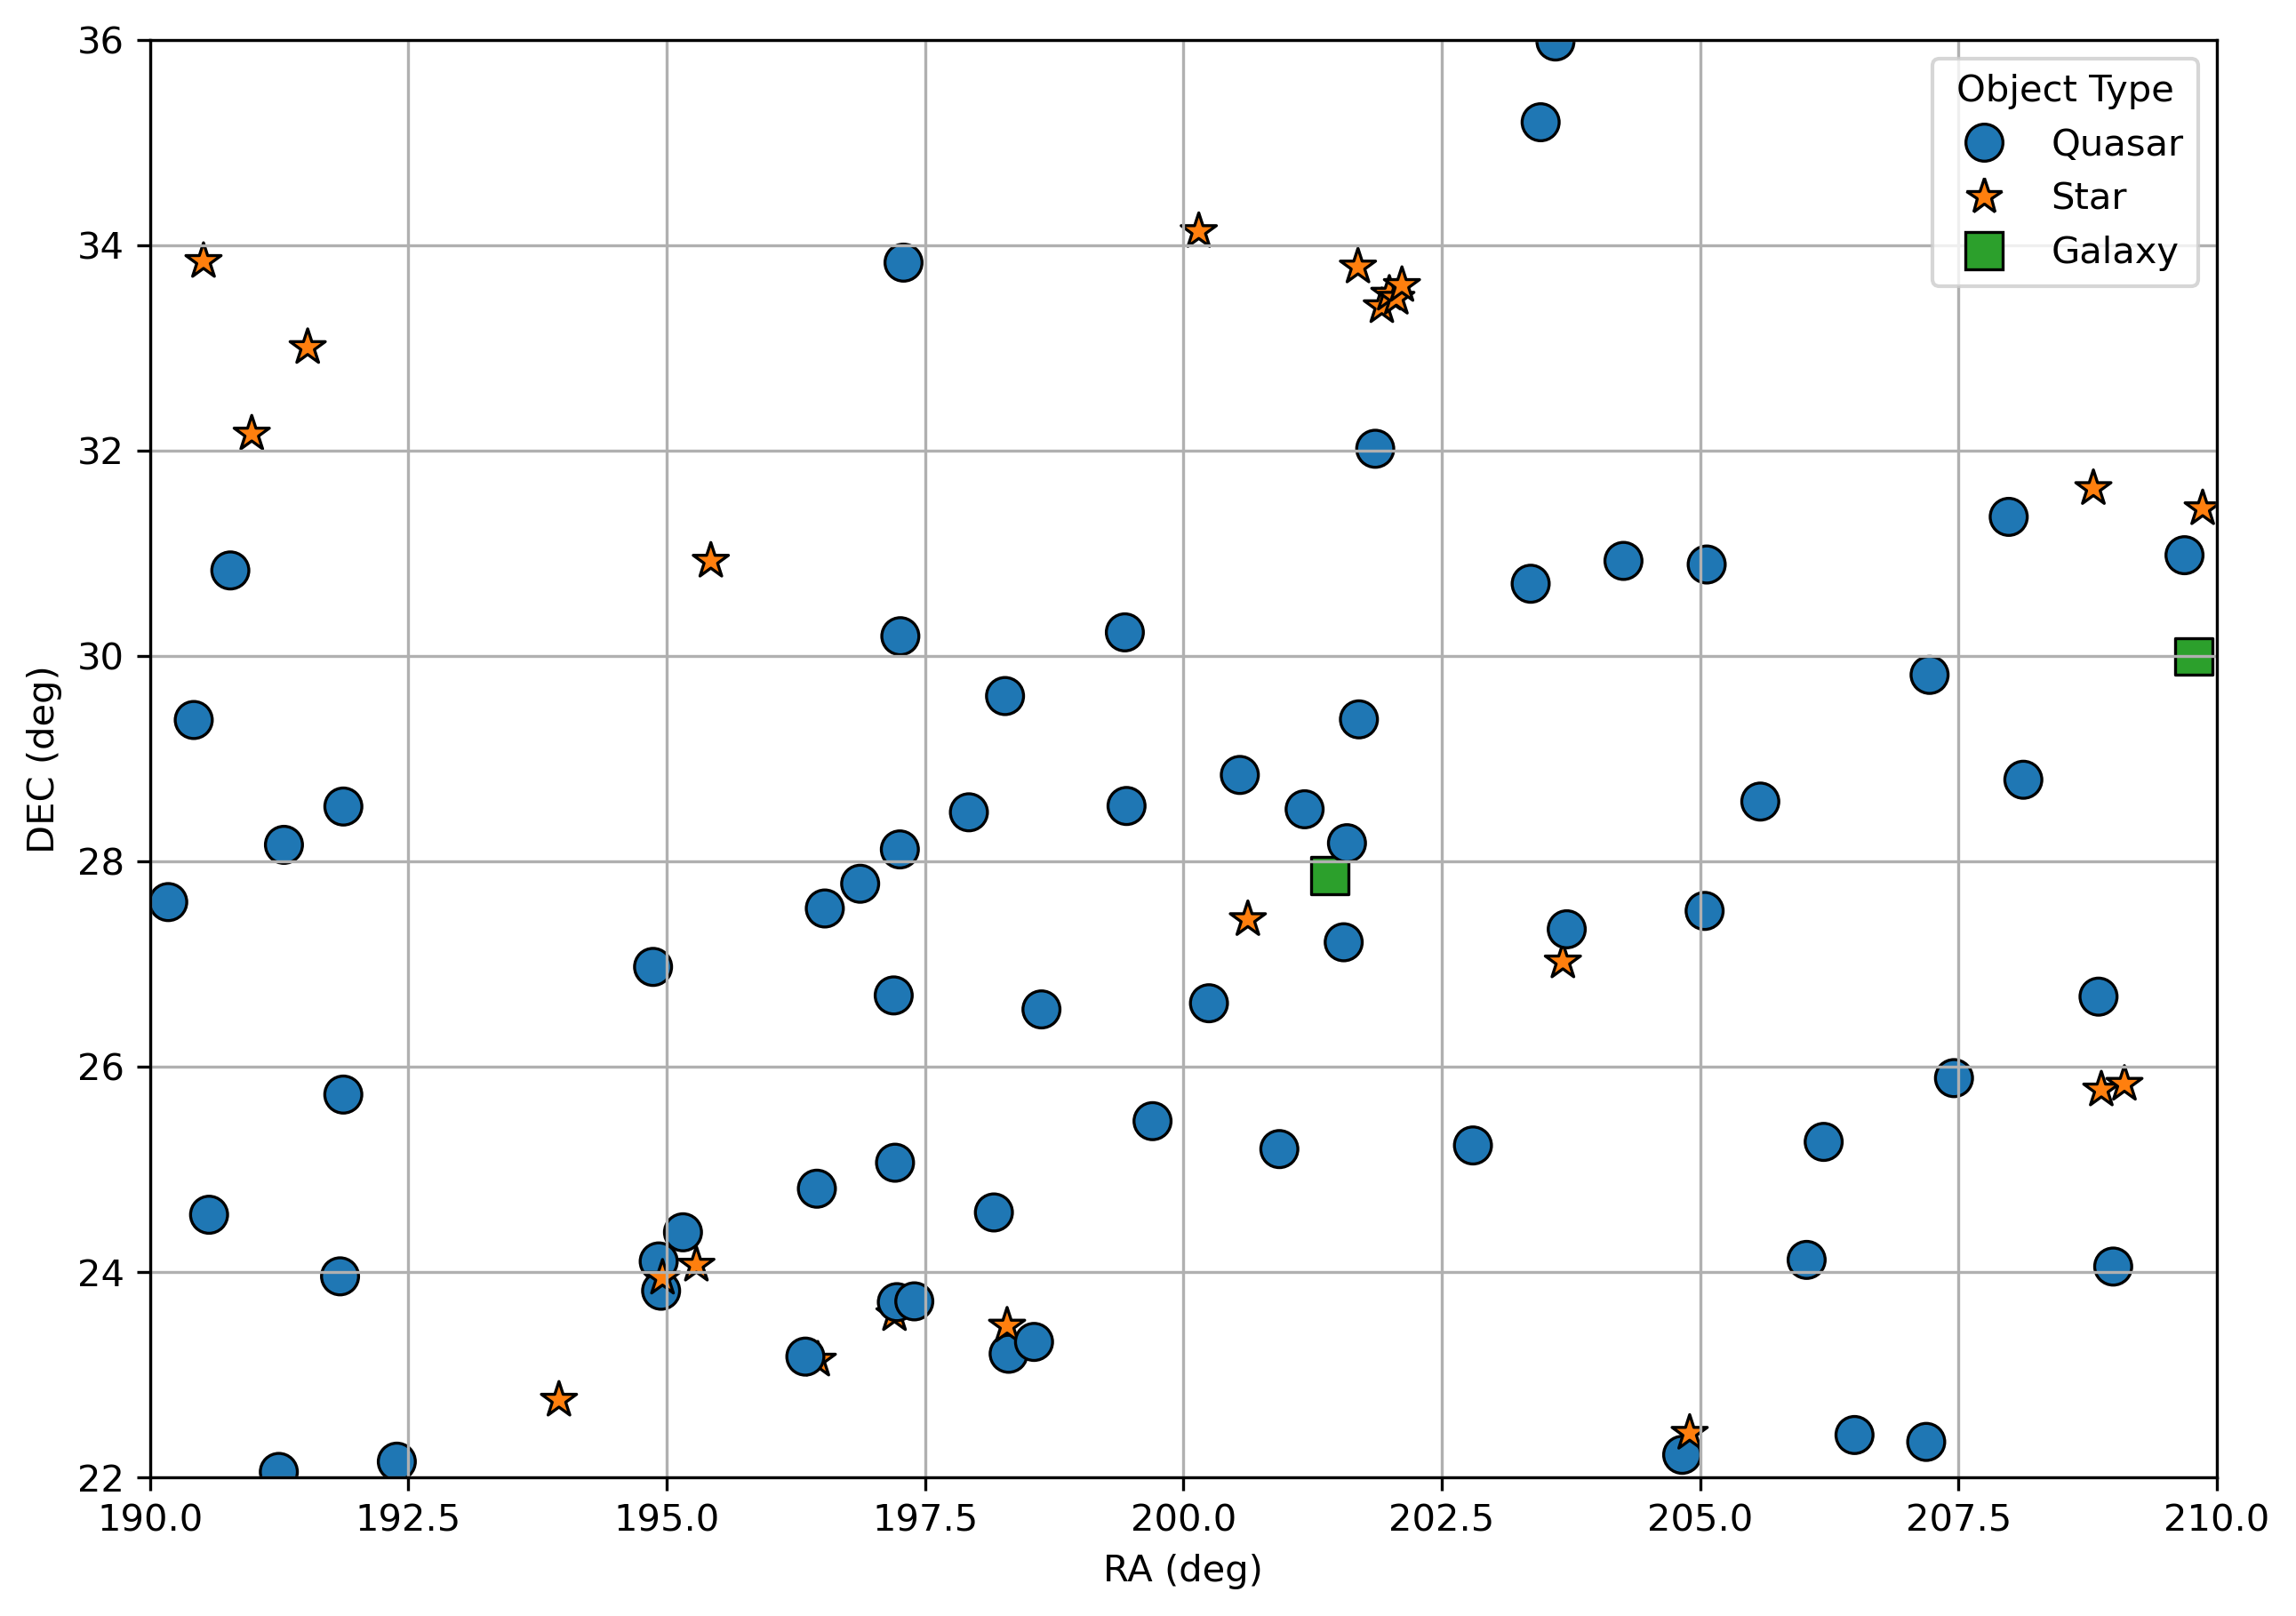
\includegraphics[width=0.9\linewidth]{figs/res/final_res_plots_type.png}
    \caption{Objects Type of 88 targets in the sky.}
    \label{fig:res_type}
\end{figure}

In Figure~\ref{fig:res_colour}, we could find quasars and other type objects are separated by the line at $\mathrm{W1}-\mathrm{W2}=0.5$. This is another useful criteria to select quasar candidates.

\begin{figure}[htbp]
    \centering
    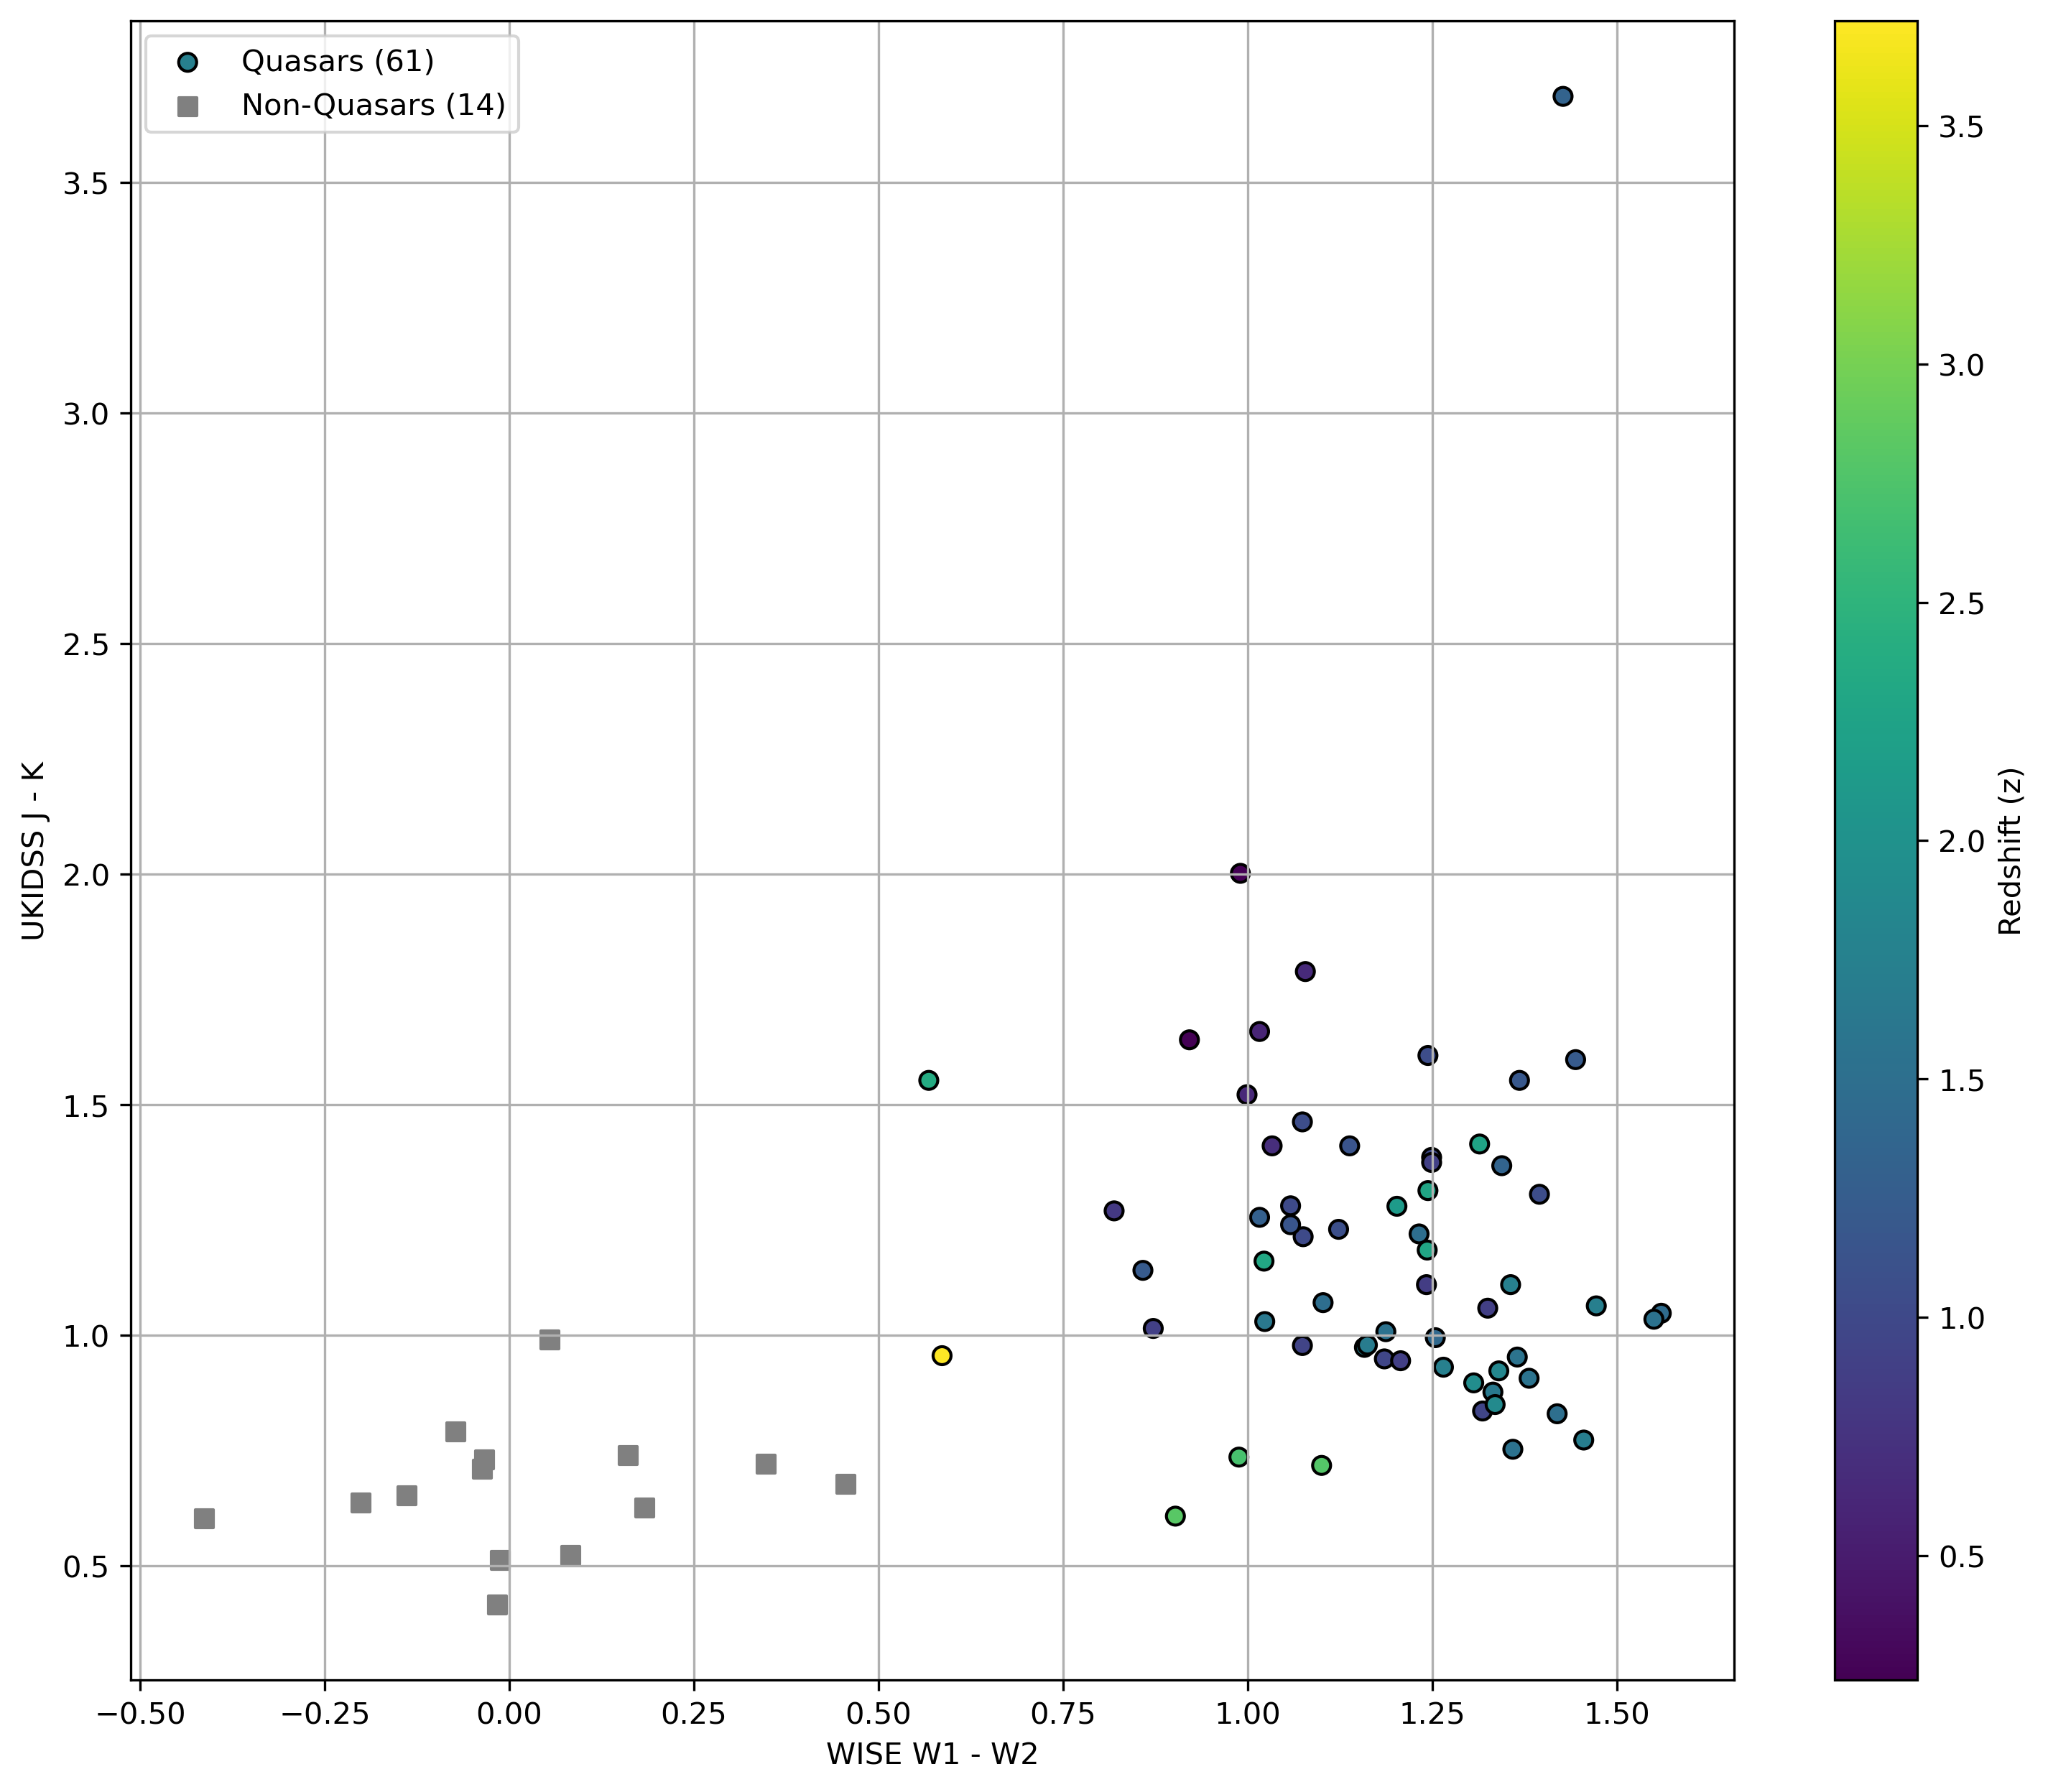
\includegraphics[width=0.75\linewidth]{figs/res/final_res_plots_color.png}
    \caption{Colour index of 75 targets. It's significant that there is a line separates quasars and other type objects at $\mathrm{W1}-\mathrm{W2}=0.5$. (Because some targets don't have photometric data from UKIDSS\citep{lawrenceUKIRTInfraredDeep2007} and/or WISE\citep{wright_wide-field_2010}, the sum of targets is lower than 88.)}
    \label{fig:res_colour}
\end{figure}

Figure~\ref{fig:z_av_joint} is the joint distribution of redshift($z$) and extinction($A_V$) for 63 quasars. The redshift values($z$) of 63 quasars are located in $0.24\sim3.72$, and most of them are around 1. Extinction($A_V$) of them is usually nearly zero, while an object has $A_V\approx3.2$ and several objects have $A_V\sim1$.

\begin{figure}[htbp]
    \centering
    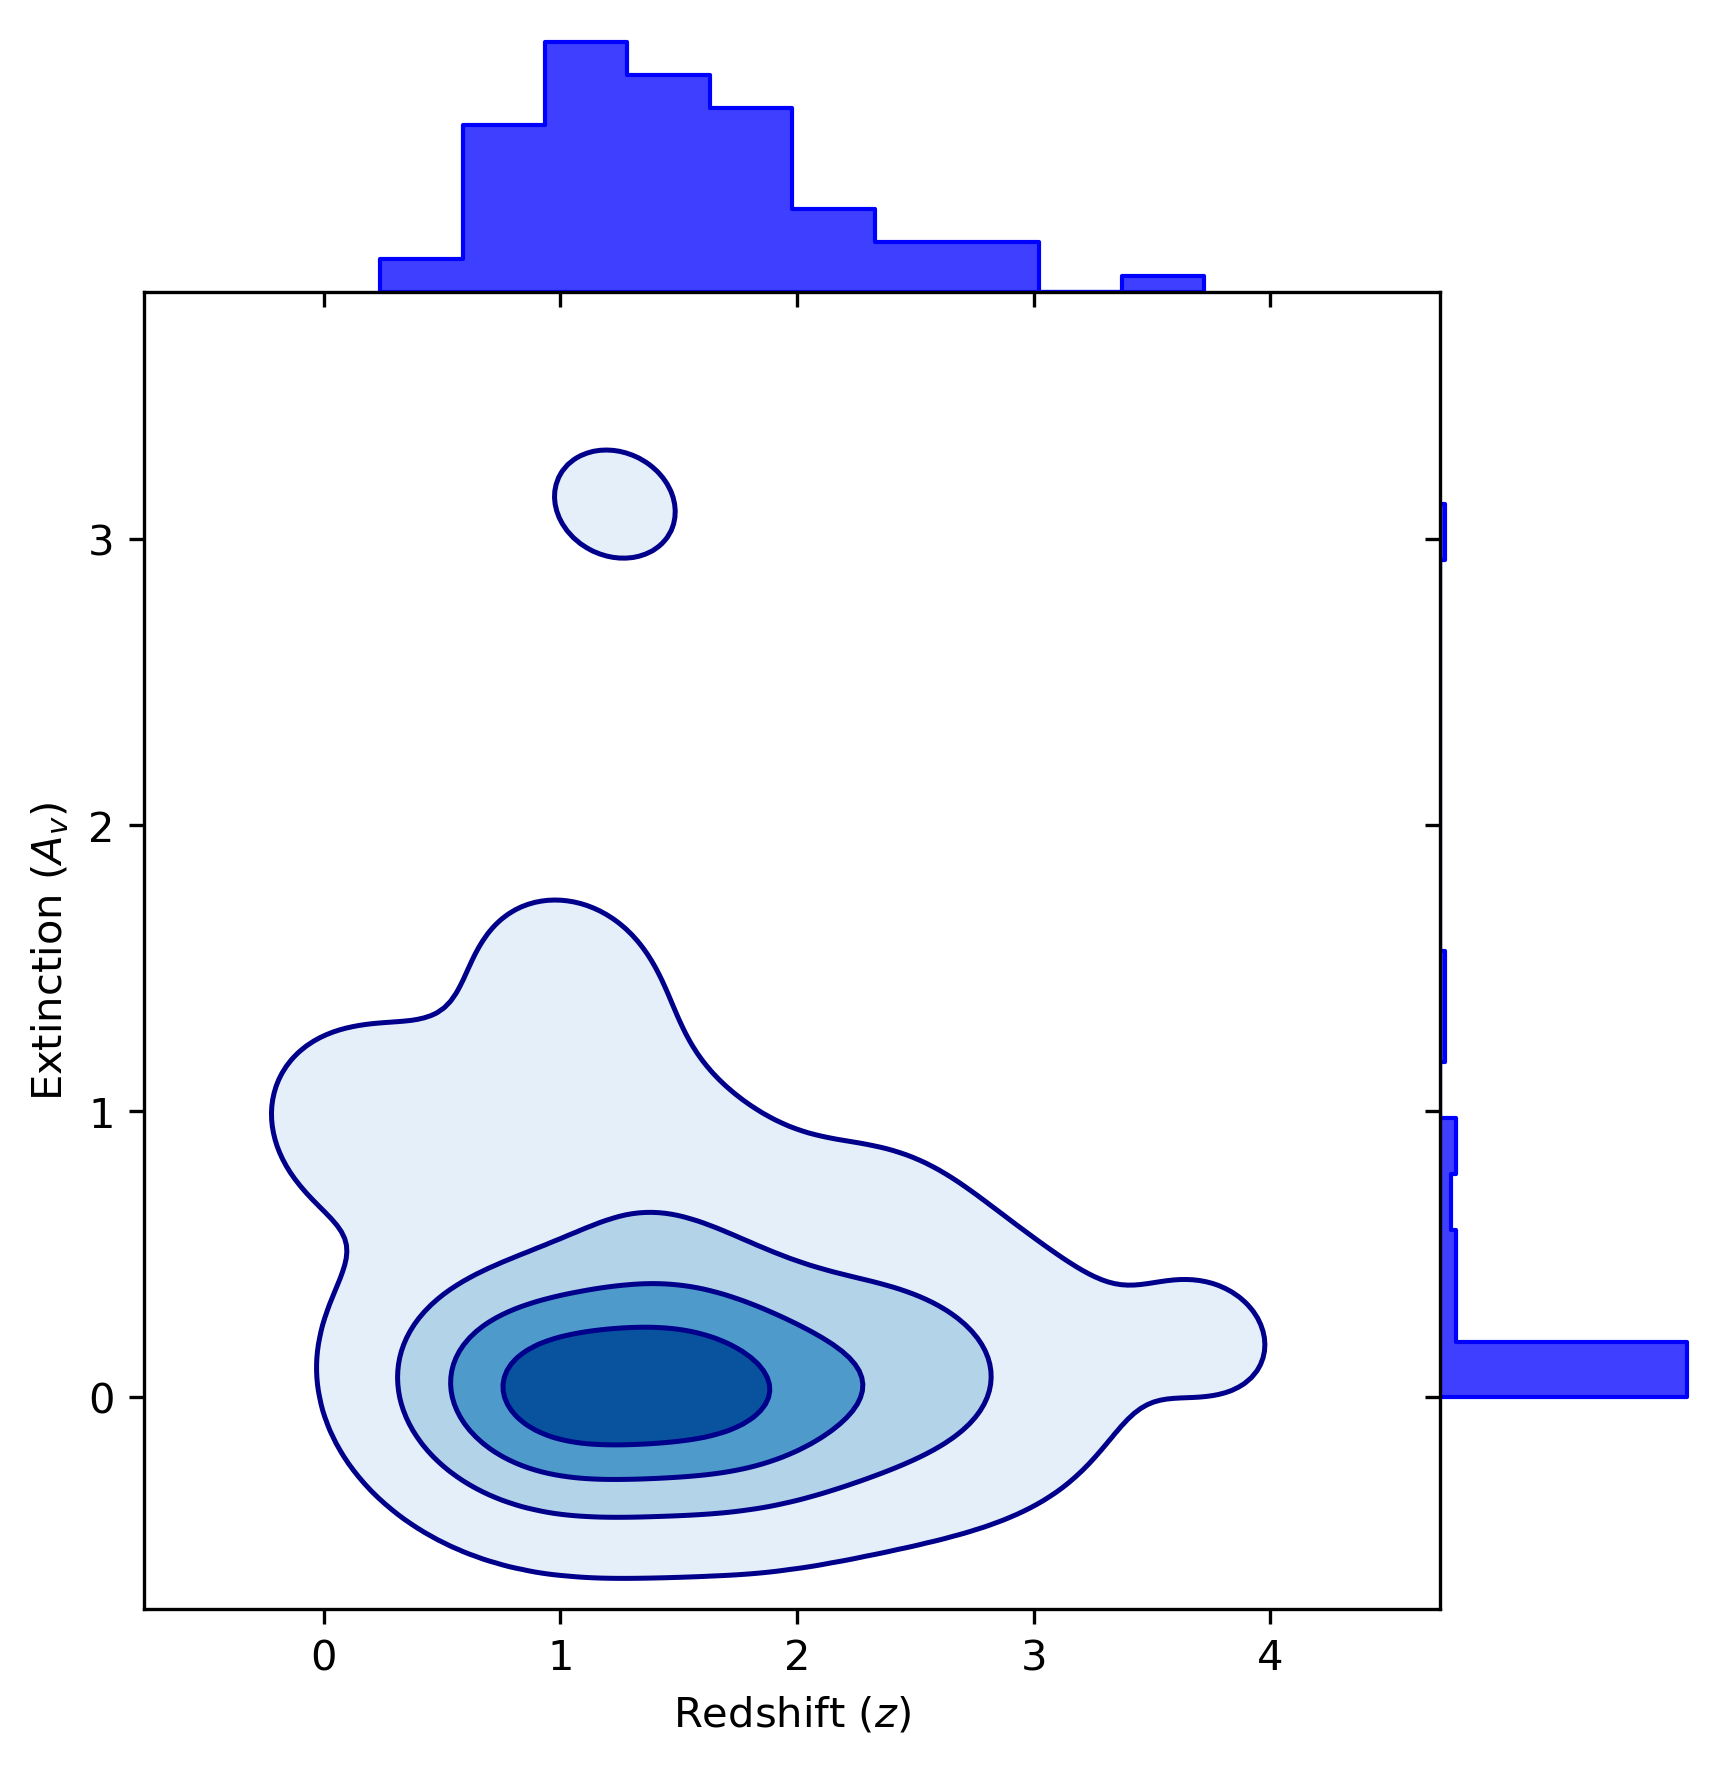
\includegraphics[width=0.9\linewidth]{figs//res/qso_z_av_joint.png}
    \caption{The Joint Distribution of Redshift($z$) and Extinction($A_v$) for 63 Quasars. Most of quasars are located in $1<z<2$ and $A_Vsim0$}
    \label{fig:z_av_joint}
\end{figure}

We also used Python package \texttt{NutMaat} \citep{nutmaat2024, mcclass2014} to automatic classify the spectra type of these 23 stars. Table~\ref{tab:obs_star_nm} is the results from automatic classification.

\begin{table}[htbp]
    \begin{tabular}{c c c c c}
    \toprule
    Target Name & Harvard Type & MK Type & Quality & $\chi^2$ \\
    \midrule
    SDSS J124204.1$+$335045.1 & G9 & V & good & 0.00 \\
    SDSS J124356.1$+$320953.6 & K2 & II & fair & 0.01 \\
    SDSS J125549.7$+$224516.4 & K2 & III-IV & fair & 0.01 \\
    SDSS J125950.2$+$235634.6 & G6 & Ia & poor & 0.10 \\
    SDSS J130108.8$+$240411.1 & F3 & Iab & - & $\infty$ \\
    SDSS J130550.9$+$230841.4 & K2 & V & fair & 0.01 \\
    SDSS J130848.9$+$233515.5 & O7 & V & fair & 0.01 \\
    SDSS J132740.9$+$332419.4 & K7 & 0 & poor & 0.14 \\
    SDSS J135513.5$+$313802.3 & G3 & Ib & good & 0.01 \\
    SDSS J135531.9$+$254633.5 & K1 & V & fair & 0.02 \\
    SDSS J135625.6$+$254952.8 & K7 & IV & good & 0.01 \\
    SDSS J135927.3$+$312614.7 & K7 & IV & good & 0.01 \\
    SDSS J124606.1$+$330027.1 & K5 & V & good & 0.04 \\
    SDSS J130142.4$+$305535.3 & - & - & - & $\infty$ \\
    SDSS J131310.5$+$232833.9 & B9.5 & V & - & 1.00 \\
    SDSS J132035.7$+$340814.6 & K7 & V & poor & 0.11 \\
    SDSS J132229.7$+$272607.4 & - & - & - & $\infty$ \\
    SDSS J132645.5$+$334731.9 & - & - & - & $\infty$ \\
    SDSS J132758.3$+$333138.1 & F6 & V & fair & 0.02 \\
    SDSS J132814.6$+$332916.6 & G4 & III & fair & 0.01 \\
    SDSS J132827.6$+$333643.2 & G3 & V & good & 0.01 \\
    SDSS J133441.4$+$270123.6 & G1 & V & good & 0.01 \\
    SDSS J133935.9$+$222555.3 & - & - & - & $\infty$ \\
    \bottomrule
    \end{tabular}
    \caption{Automatic Classify Results of 23 Stars by \texttt{nutmaat}}
    \label{tab:obs_star_nm}
\end{table}

\section{Results from Observations}

All spectra we observed are in Appendix~\ref{app:raw}.

\subsection{Quasars}

The spectrum of a normal quasar is like Figure~\ref{fig:normal_qso}. This spectrum is from \textbf{SDSS~J130935.0$+$234256.5}, a normal quasar at $z=1.85$. Following, we will introduce some special quasars in our observations.

\begin{figure}[htbp]
    \centering
    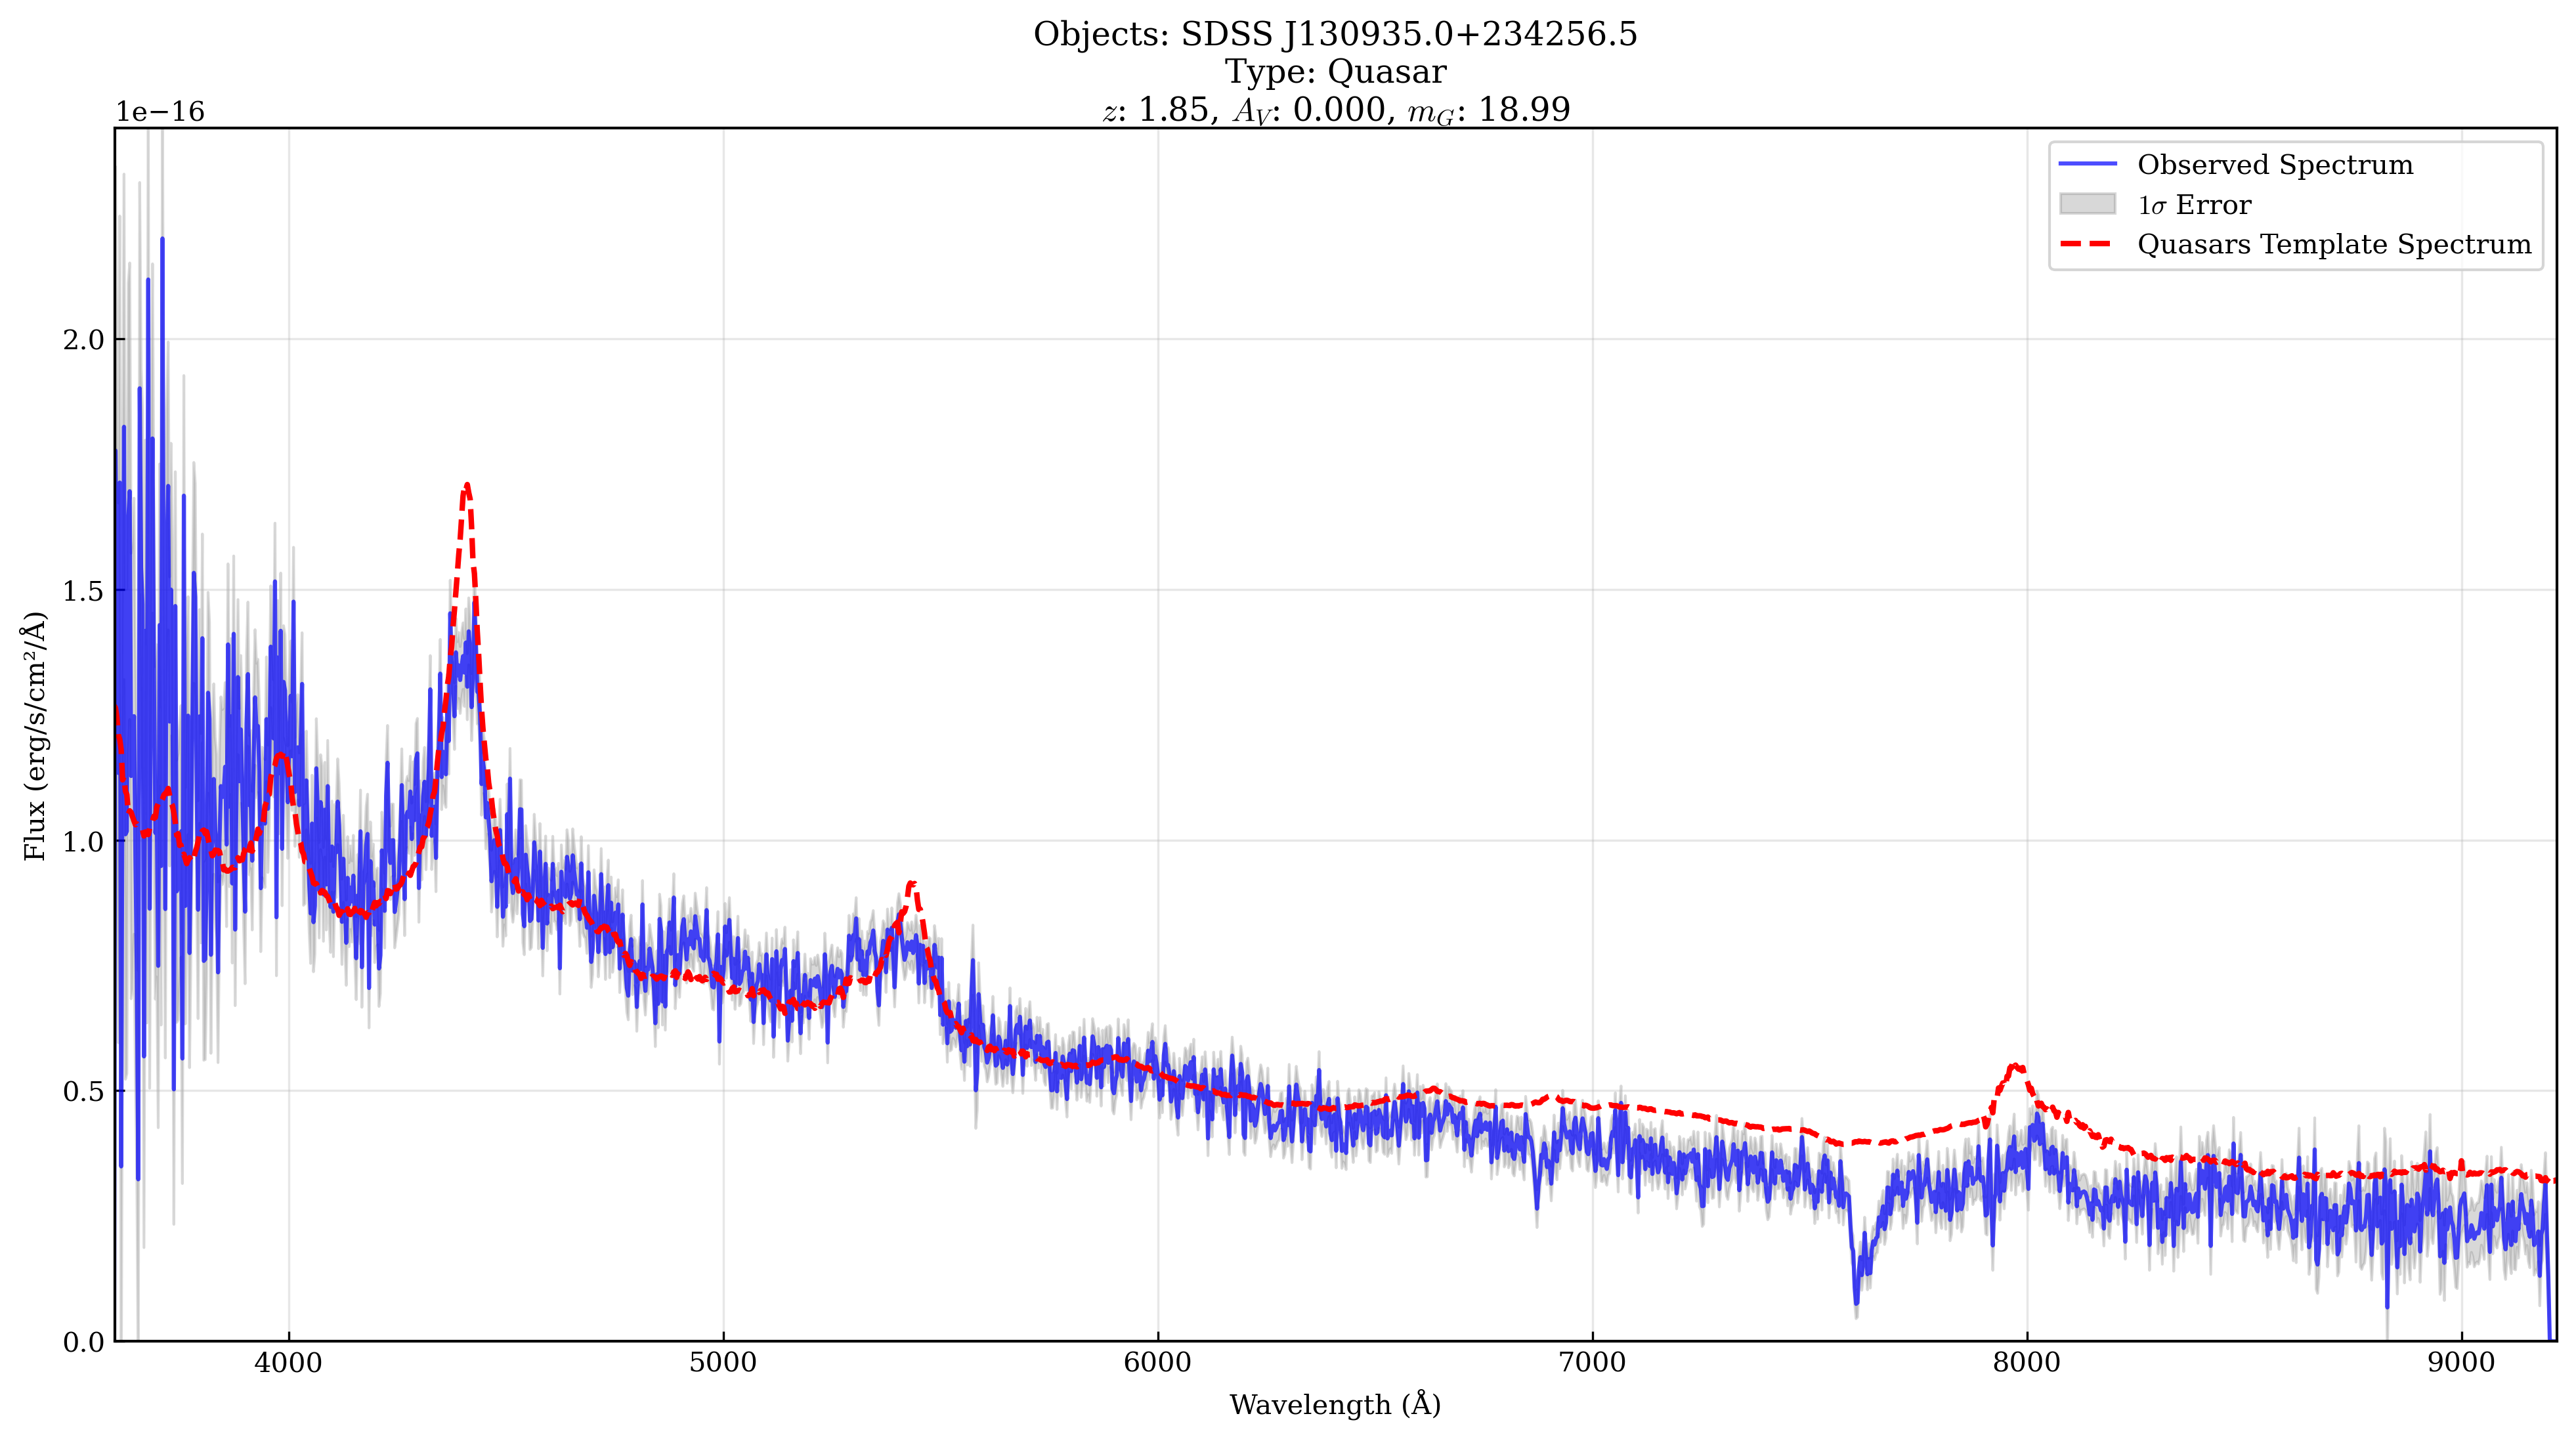
\includegraphics[width=0.9\linewidth]{figs//raw/SDSS_J130935+234256.png}
    \caption{The target \textbf{SDSS~J130935.0$+$234256.5} is a sample of Normal Quasars at $z=1.85$}
    \label{fig:normal_qso}
\end{figure}

The target \textbf{SDSS~J124306.4$+$305005.2}(Figure~\ref{fig:low_z_qso}) has the lowest redshift $z=0.24$ among the 63 quasars. And the target with highest redshift $z=3.72$ is \textbf{SDSS~J132647.7$+$292303.5}(Figure~\ref{fig:high_z_qso})

\begin{figure}[htbp]
    \centering
    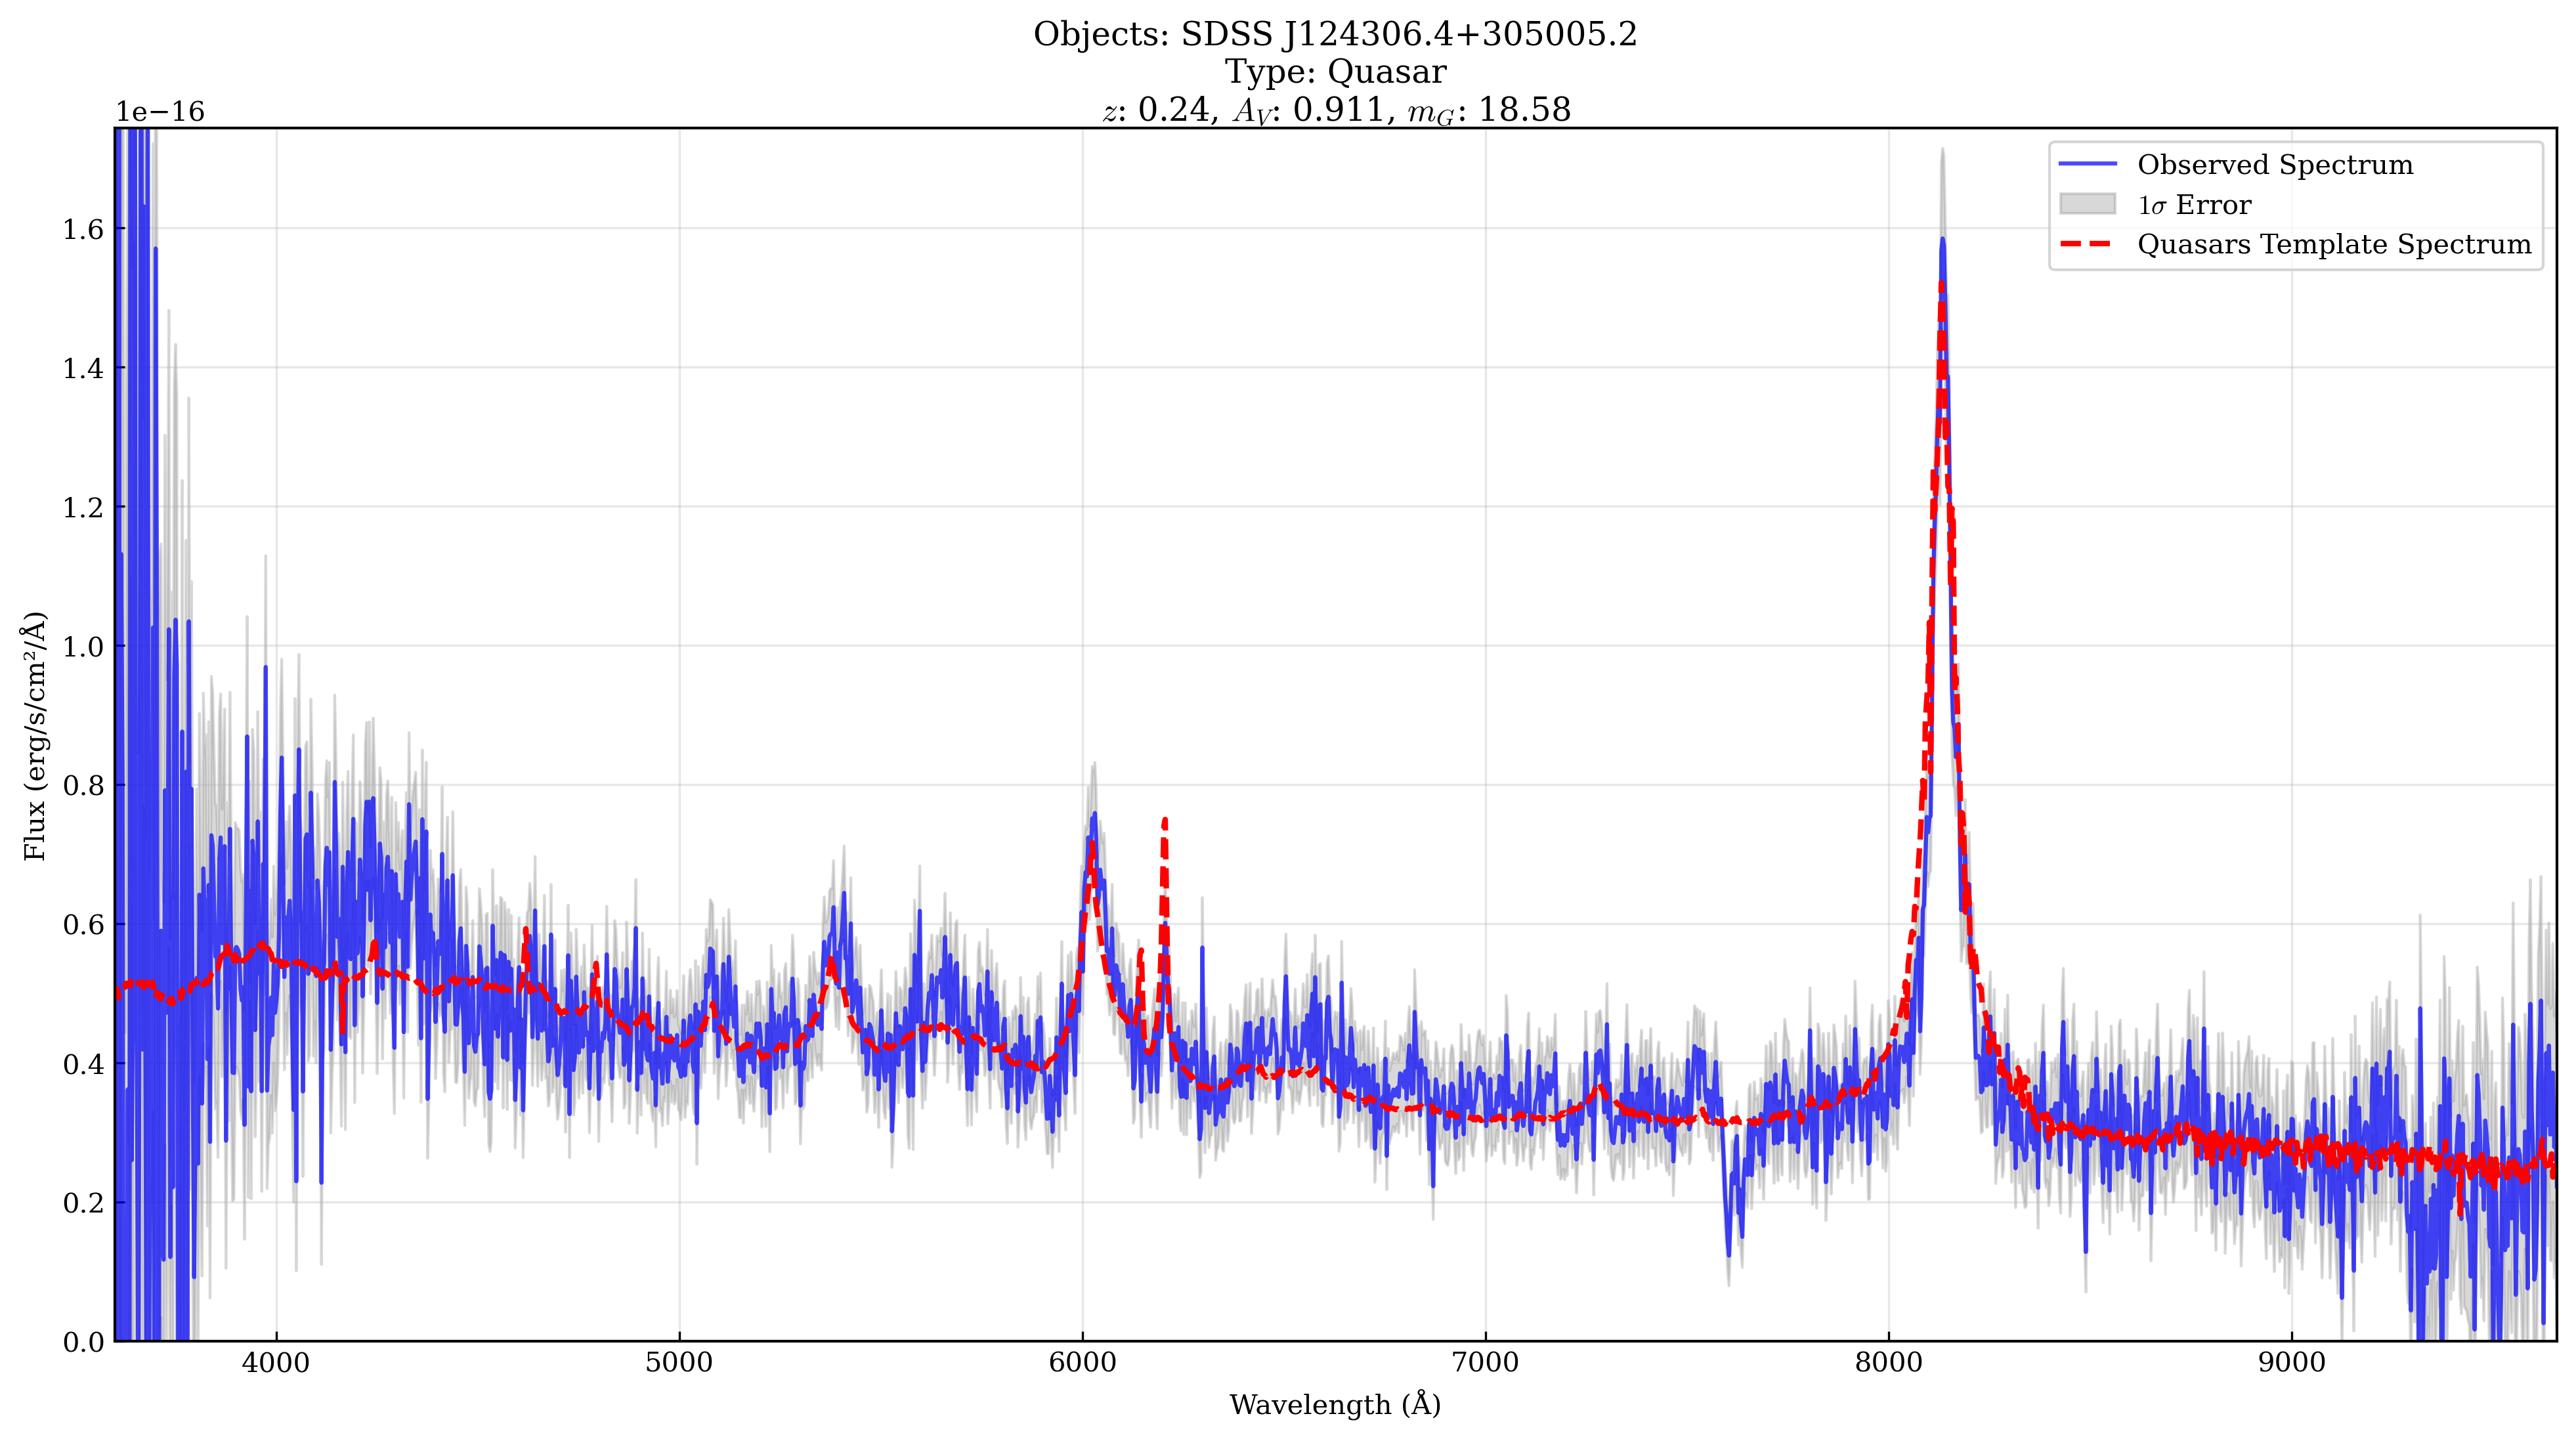
\includegraphics[width=0.9\linewidth]{figs//raw/SDSS_J124306+305005.png}
    \caption{The target \textbf{SDSS~J124306.4$+$305005.2} with the Lowest Redshift $z=0.24$}
    \label{fig:low_z_qso}
\end{figure}

\begin{figure}[htbp]
    \centering
    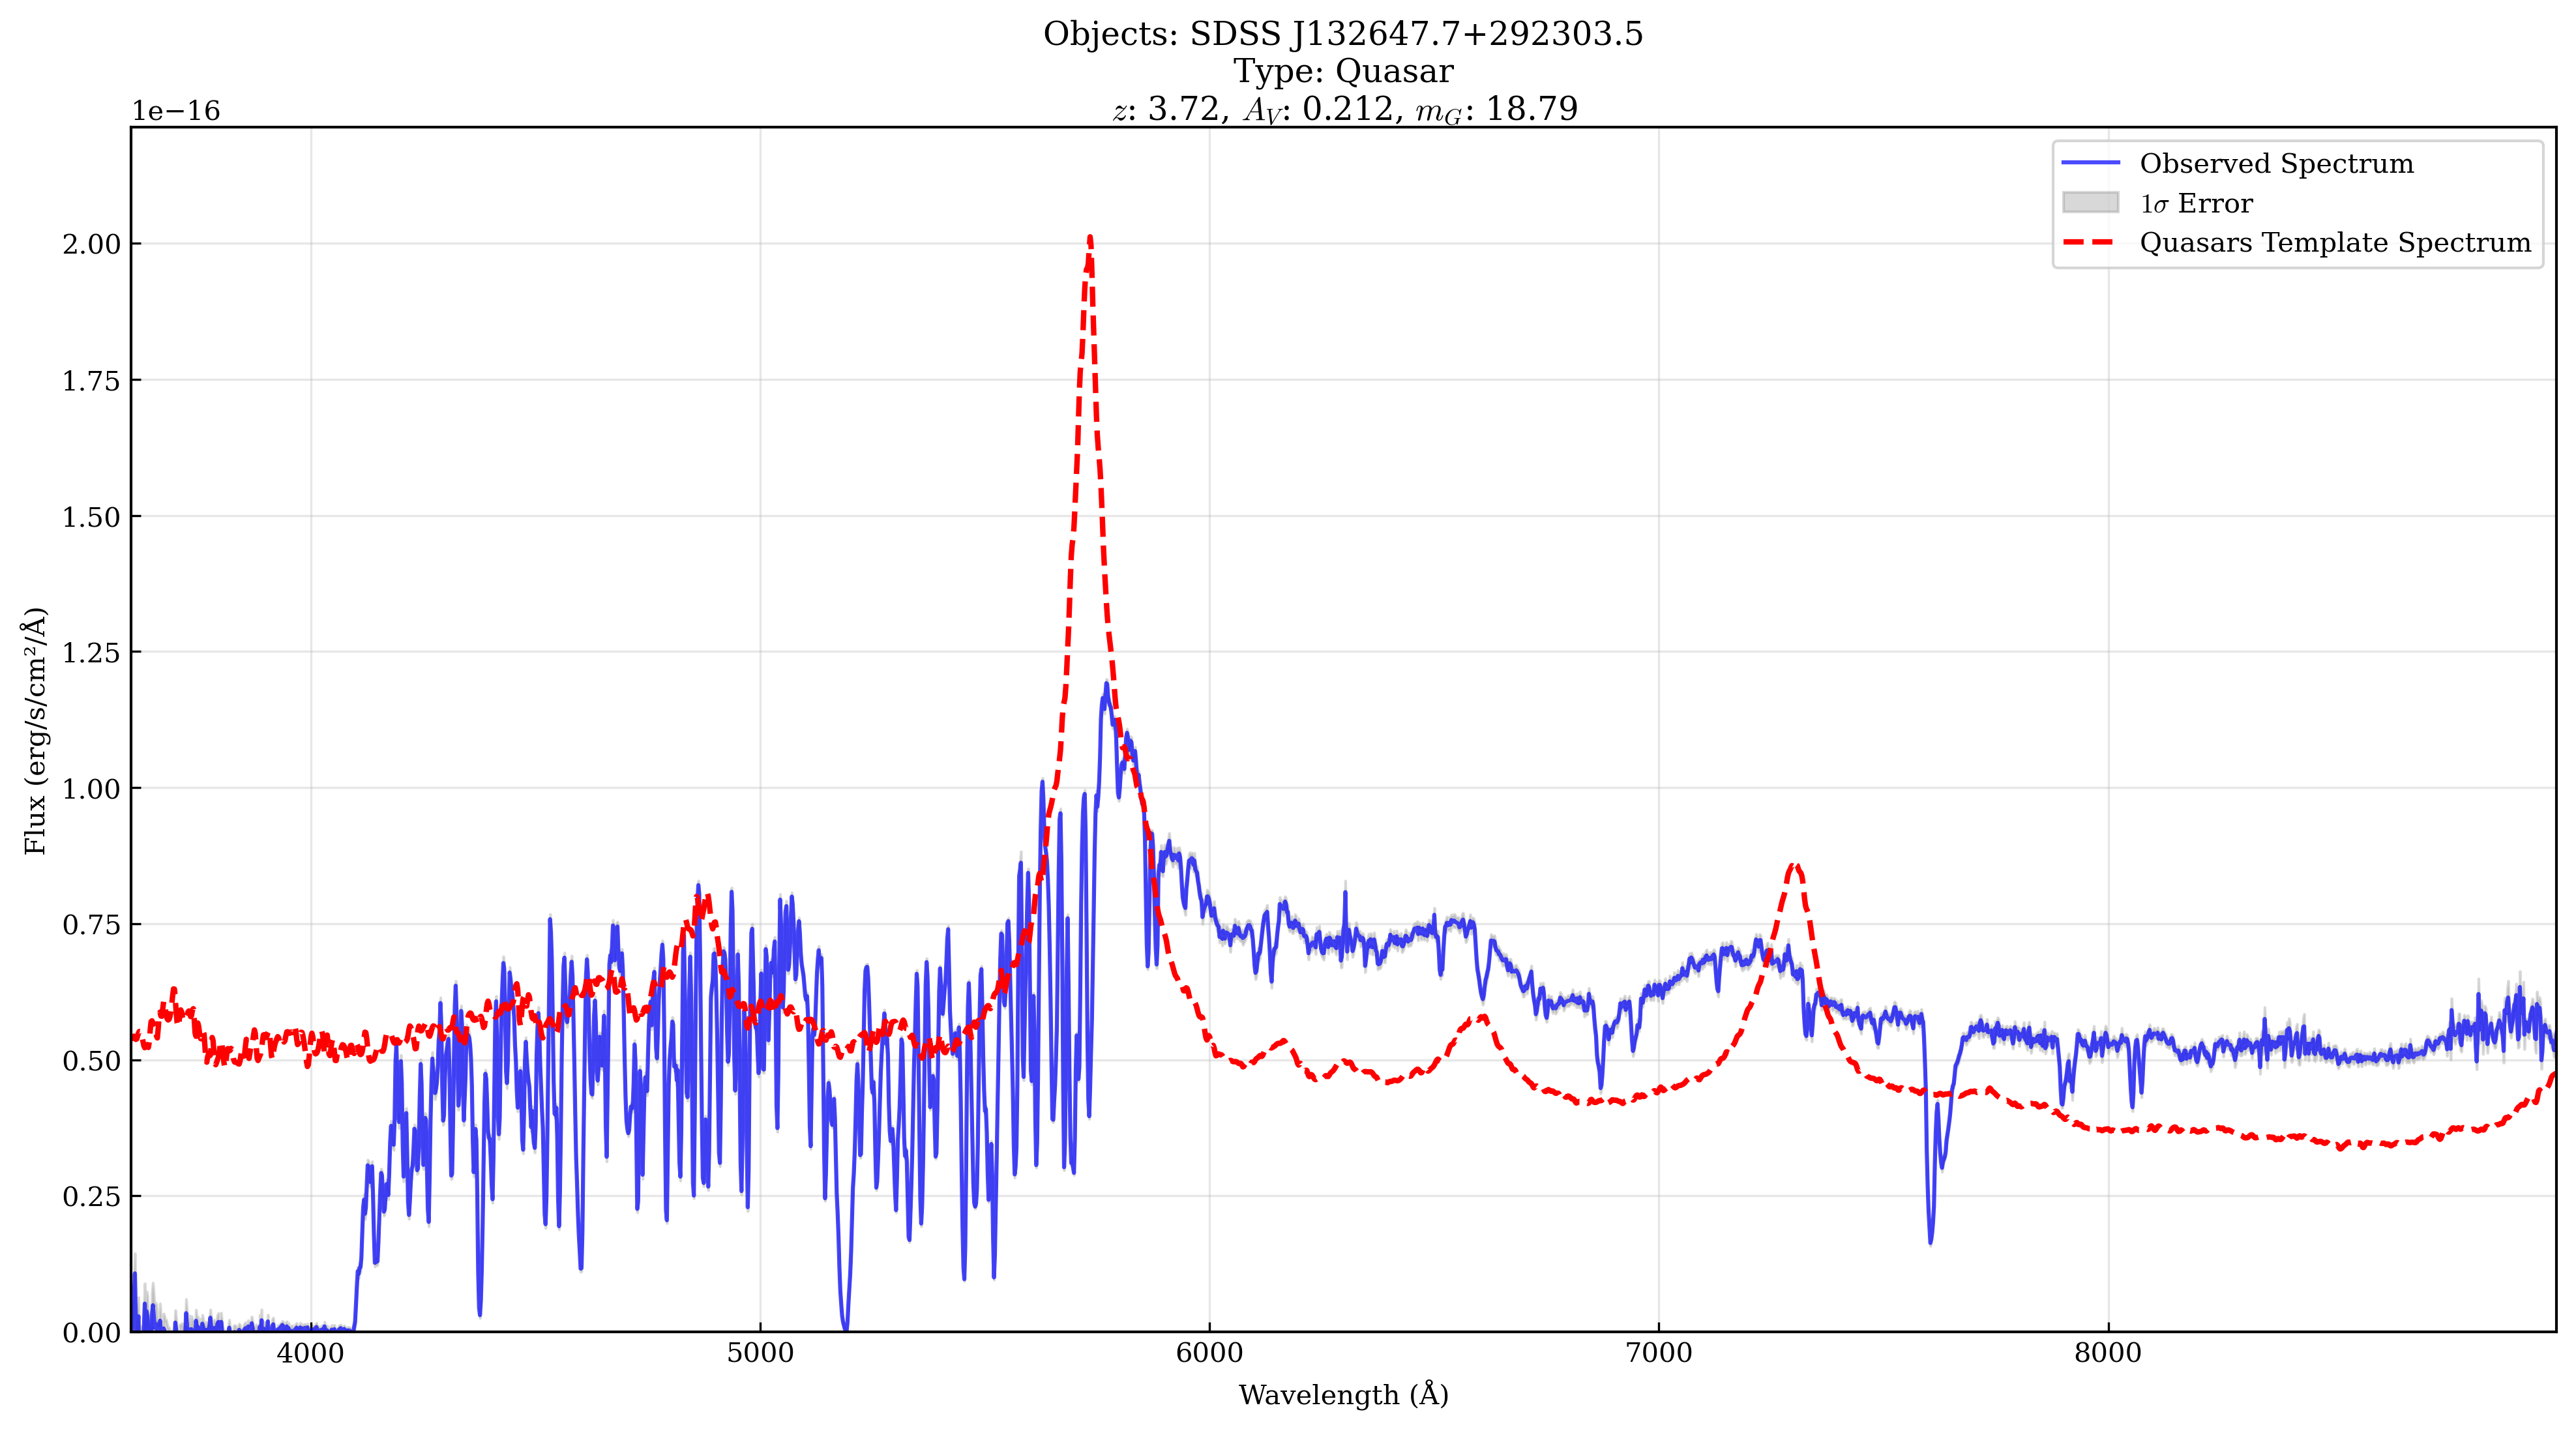
\includegraphics[width=0.9\linewidth]{figs//raw/SDSS_J132647+292303.png}
    \caption{The target \textbf{SDSS~J132647.7$+$292303.5} with the Highest Redshift $z=3.72$}
    \label{fig:high_z_qso}
\end{figure}

Also, \textbf{SDSS~J132647.7$+$292303.5} is a unusual quasar. It doesn't have strong emission lines. We think the reason may be the absorption from the host galaxy disk. 

While most of observed quasars just have extinction in $0\leq A_V\leq 0.25$, \textbf{SDSS~J134010.6$+$273106.2} (Figure~\ref{fig:highest_av_qso}) shows a very strong extinction in blue end of spectrum ($A_V\approx3.2$).
\begin{figure}[htbp]
    \centering
    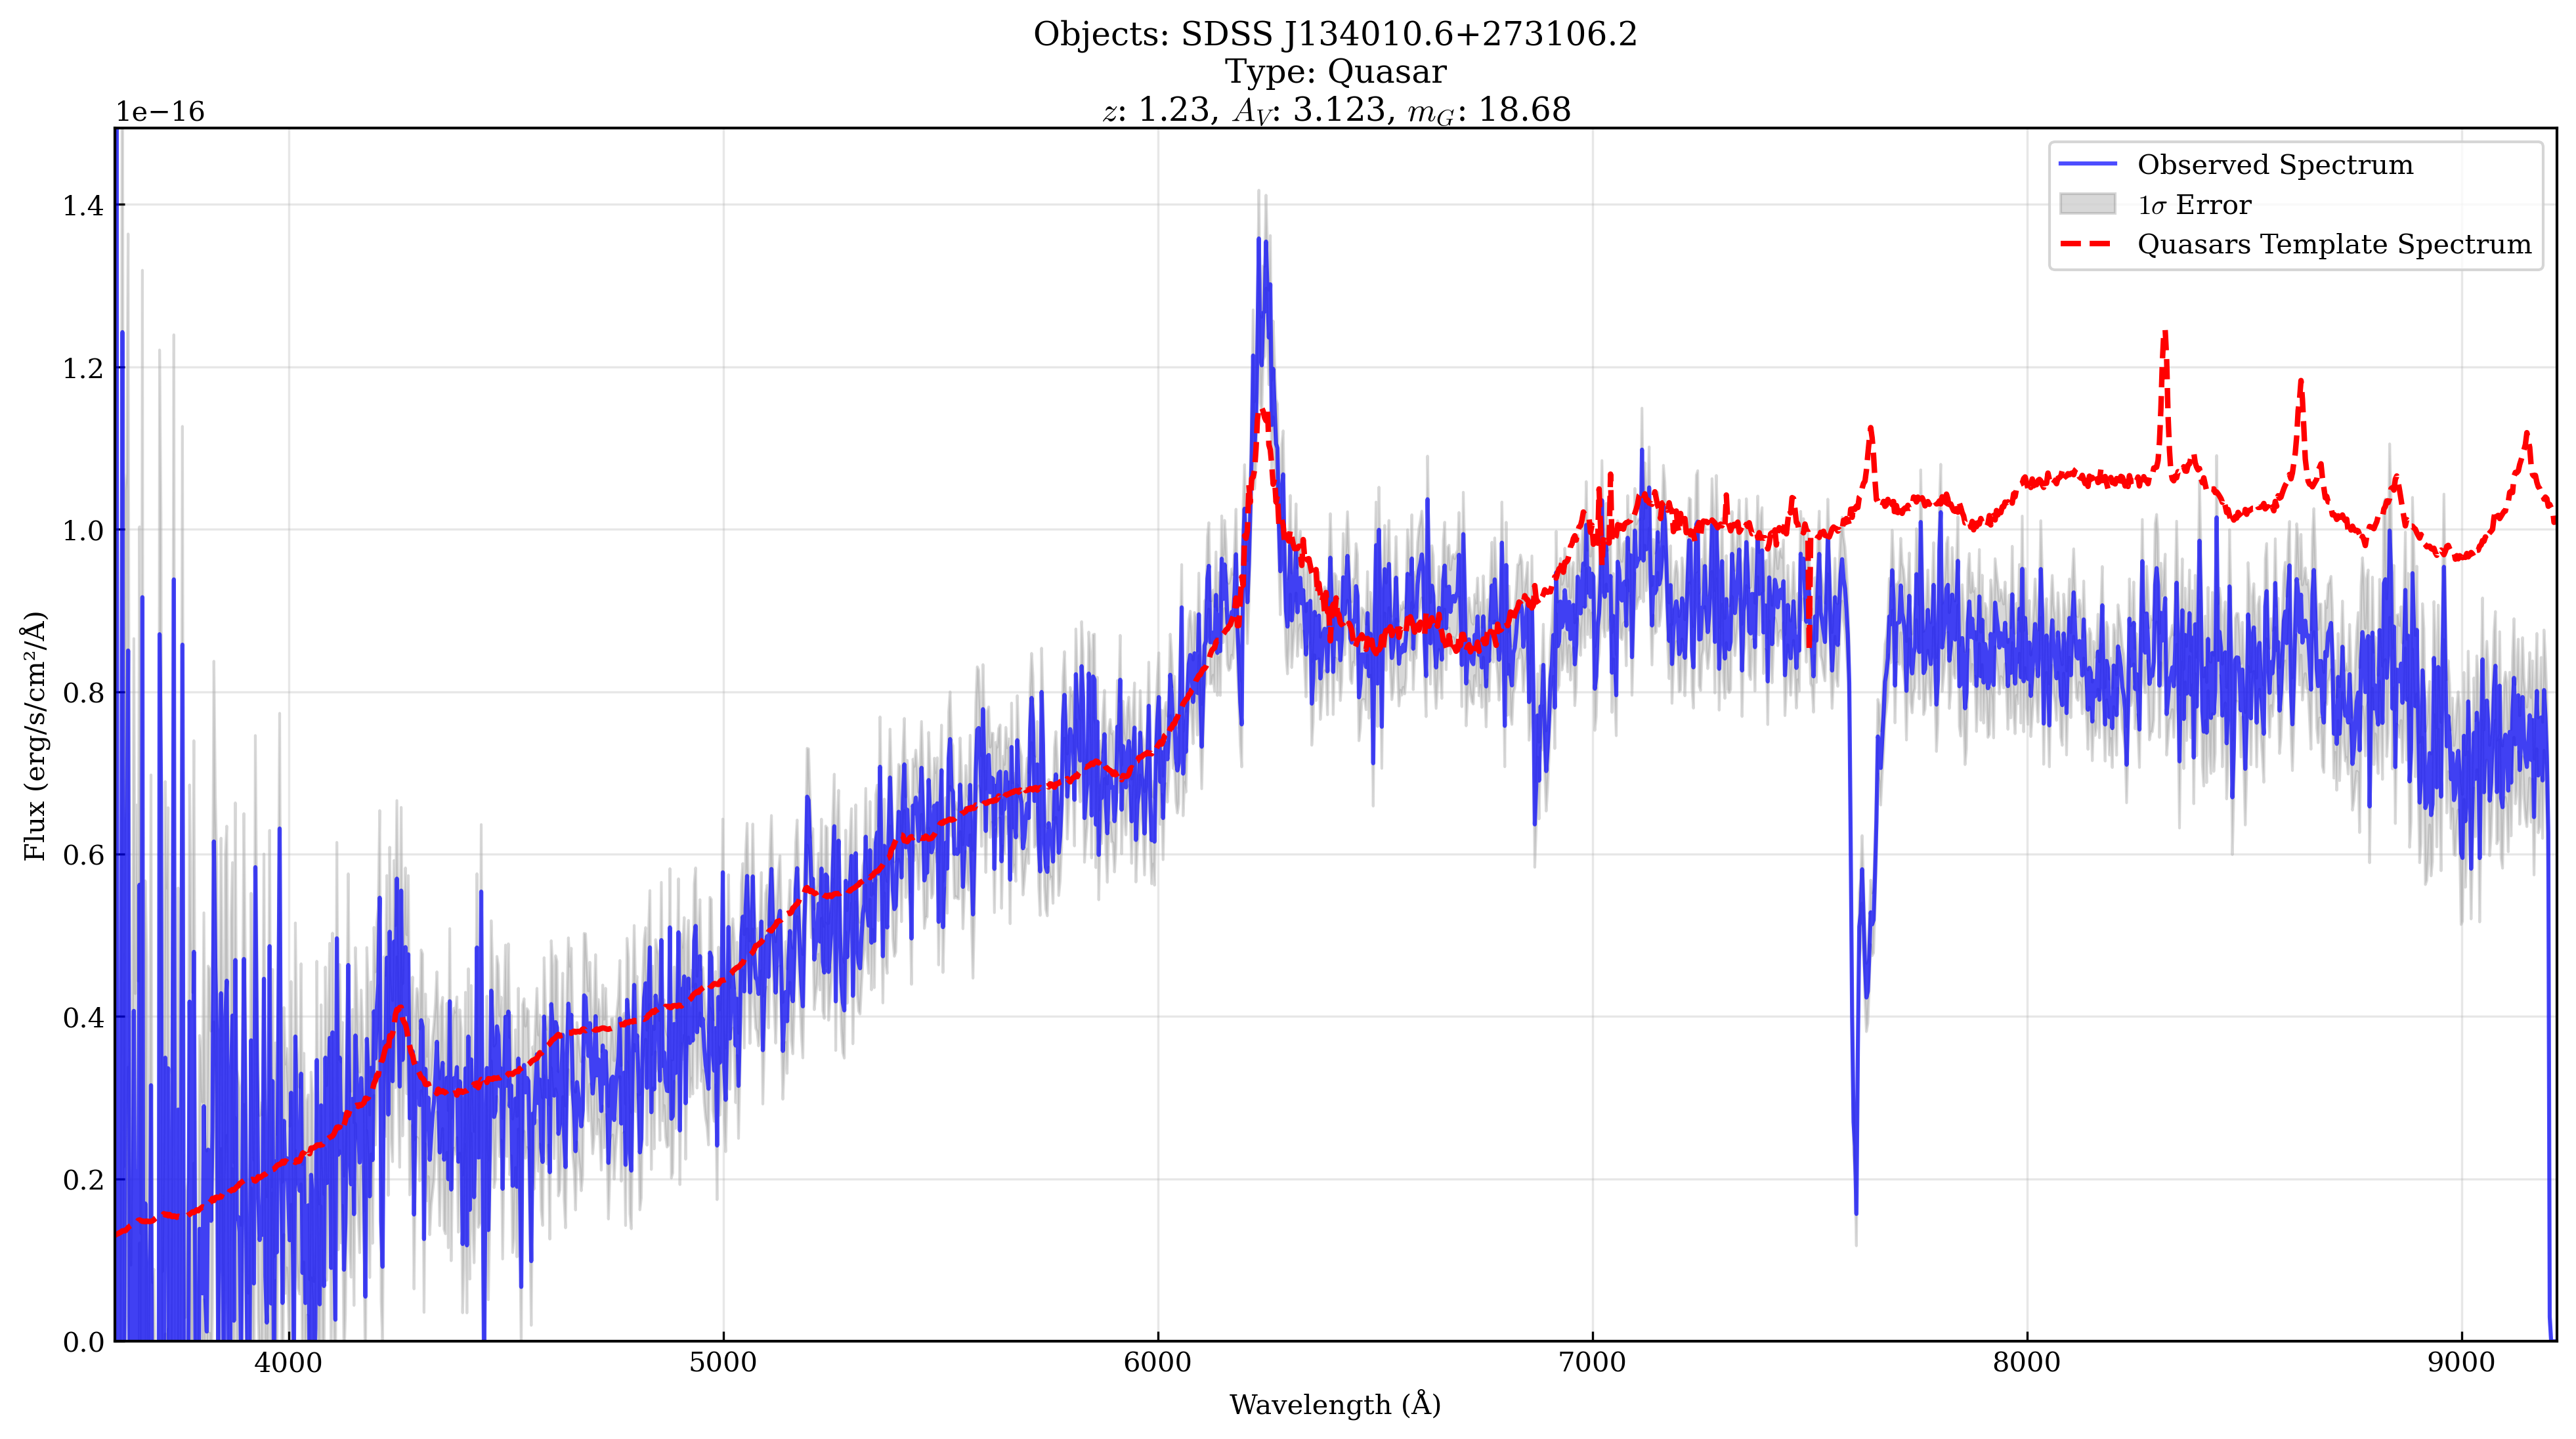
\includegraphics[width=0.9\linewidth]{figs//raw/SDSS_J134010+273106.png}
    \caption{The target \textbf{SDSS~J134010.6$+$273106.2} with the Highest Extinction $A_V=3.12$}
    \label{fig:highest_av_qso}
\end{figure}

\begin{figure}[htbp]
    \centering
    \begin{subfigure}[b]{0.45\textwidth}
        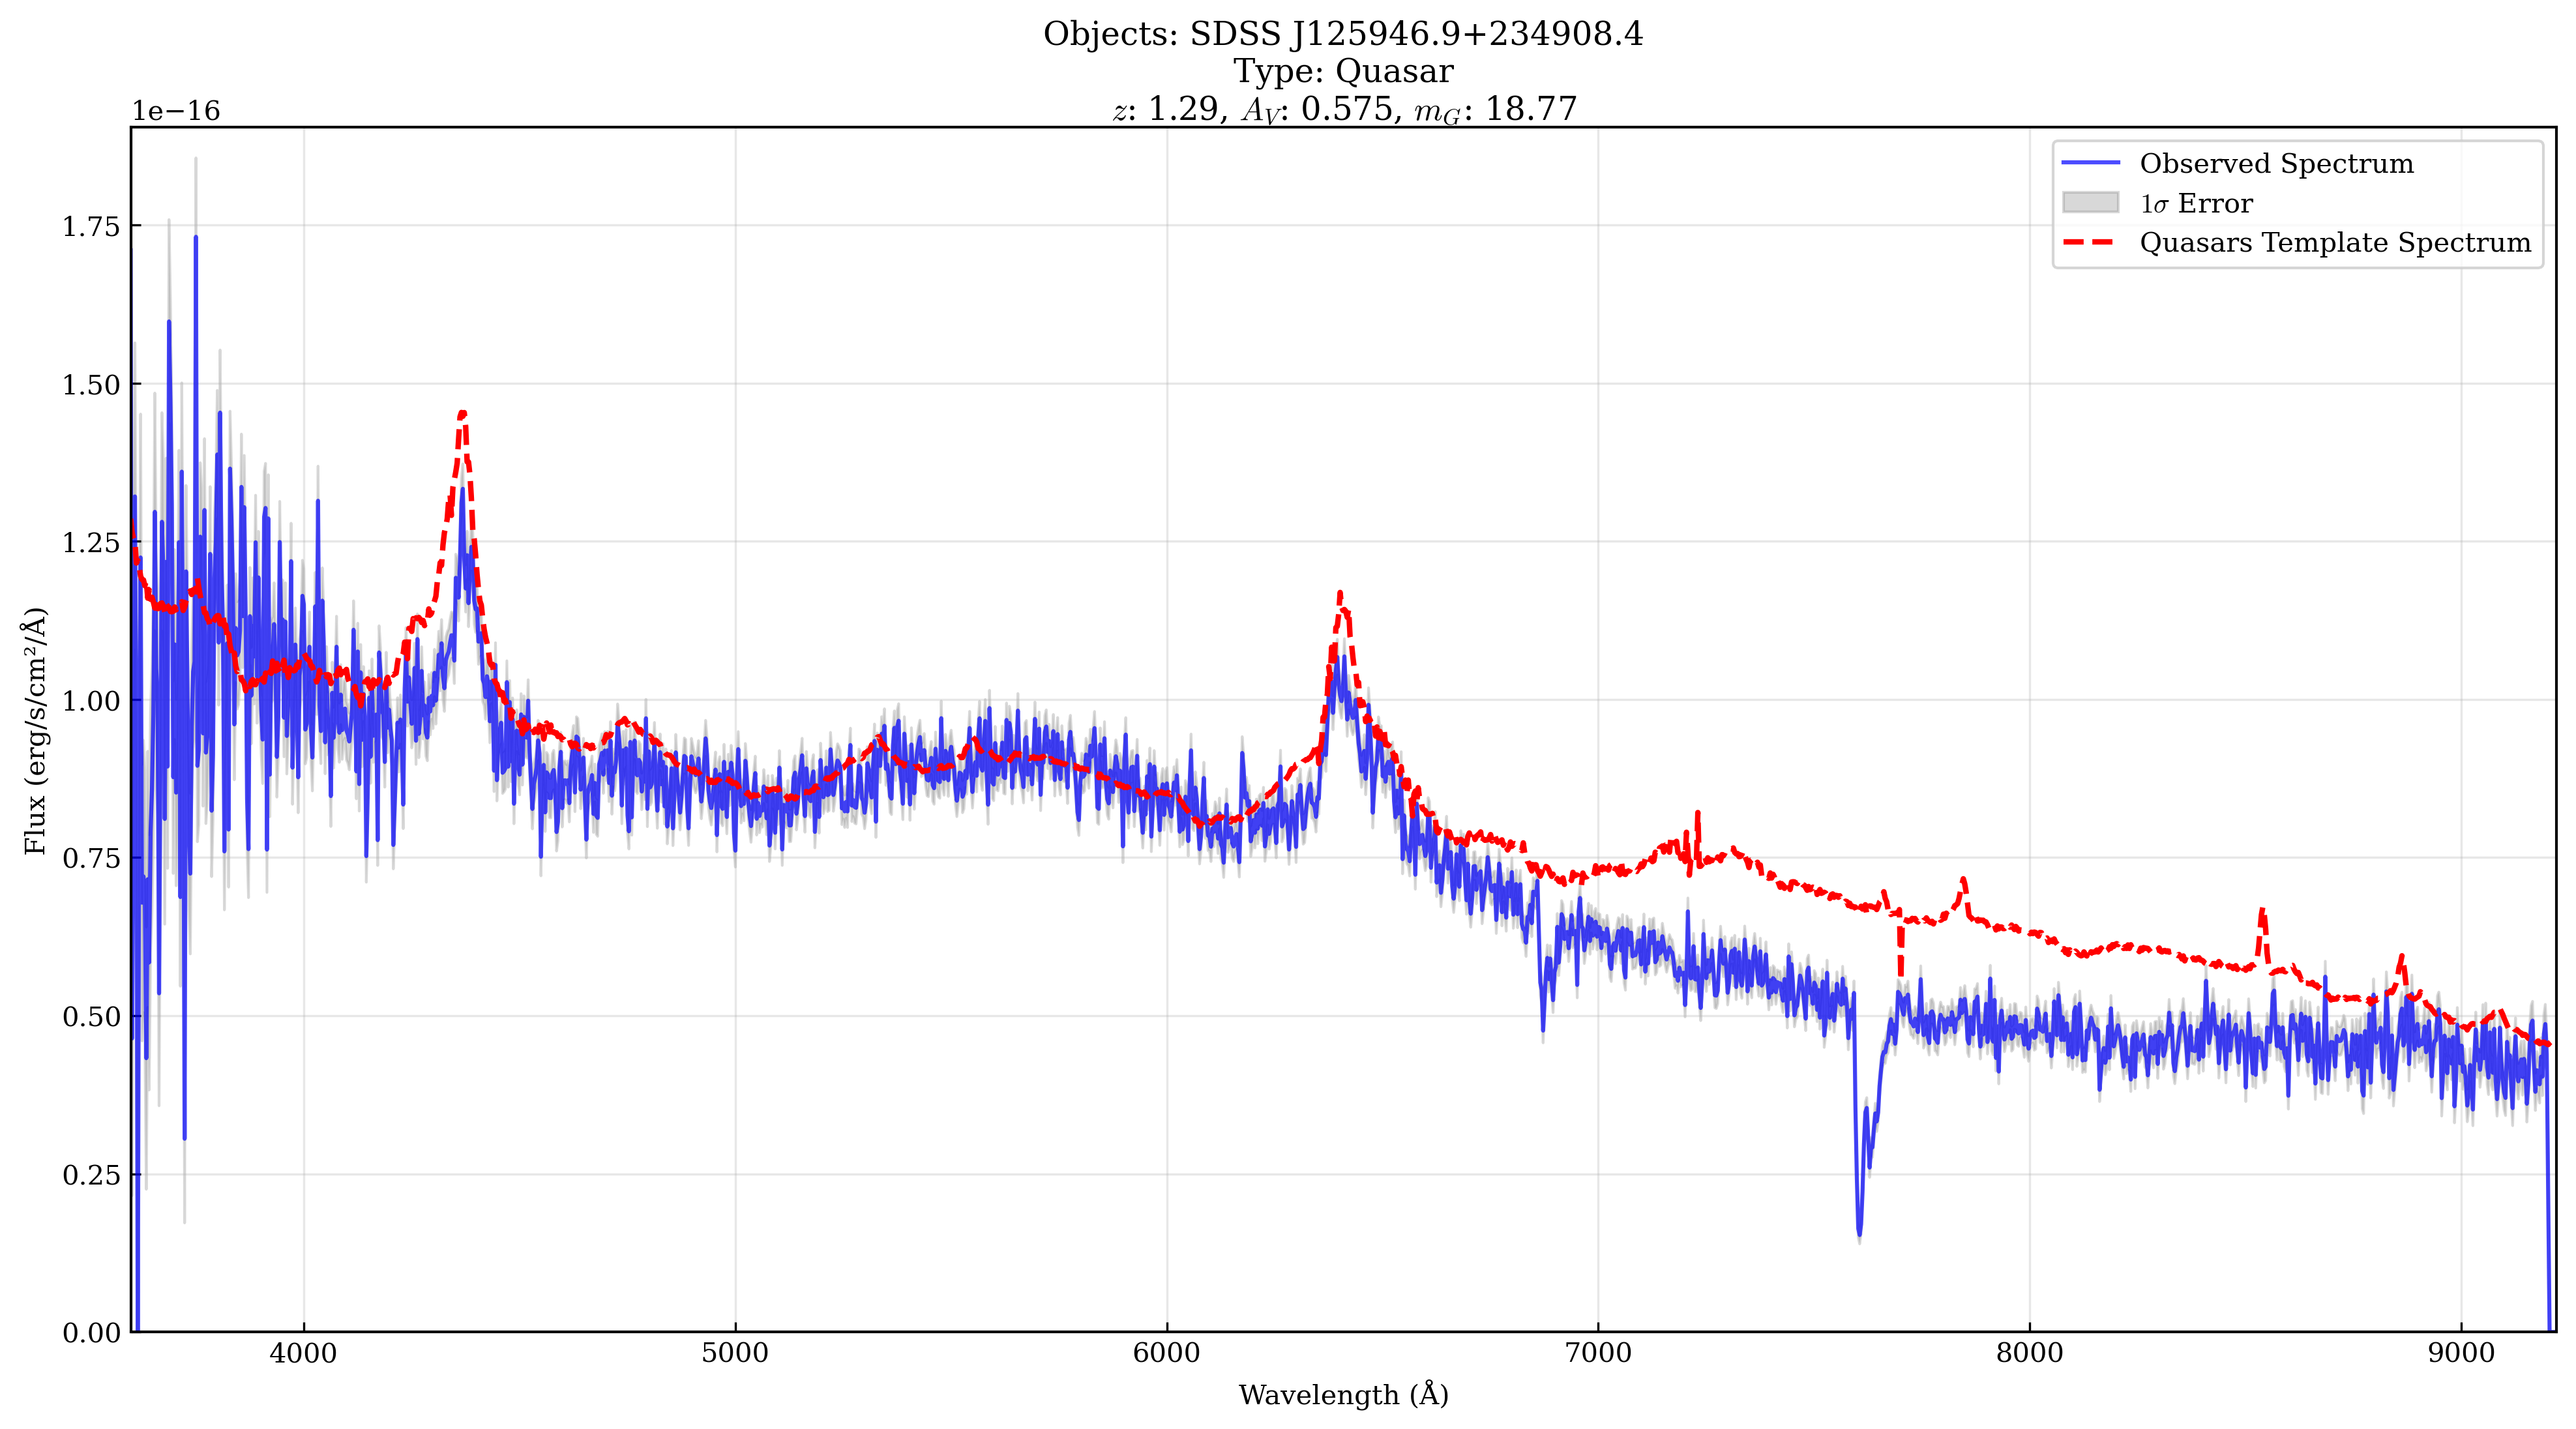
\includegraphics[width=\linewidth]{figs//raw/SDSS_J125946+234908.png}
    \end{subfigure}
    \begin{subfigure}[b]{0.45\textwidth}
        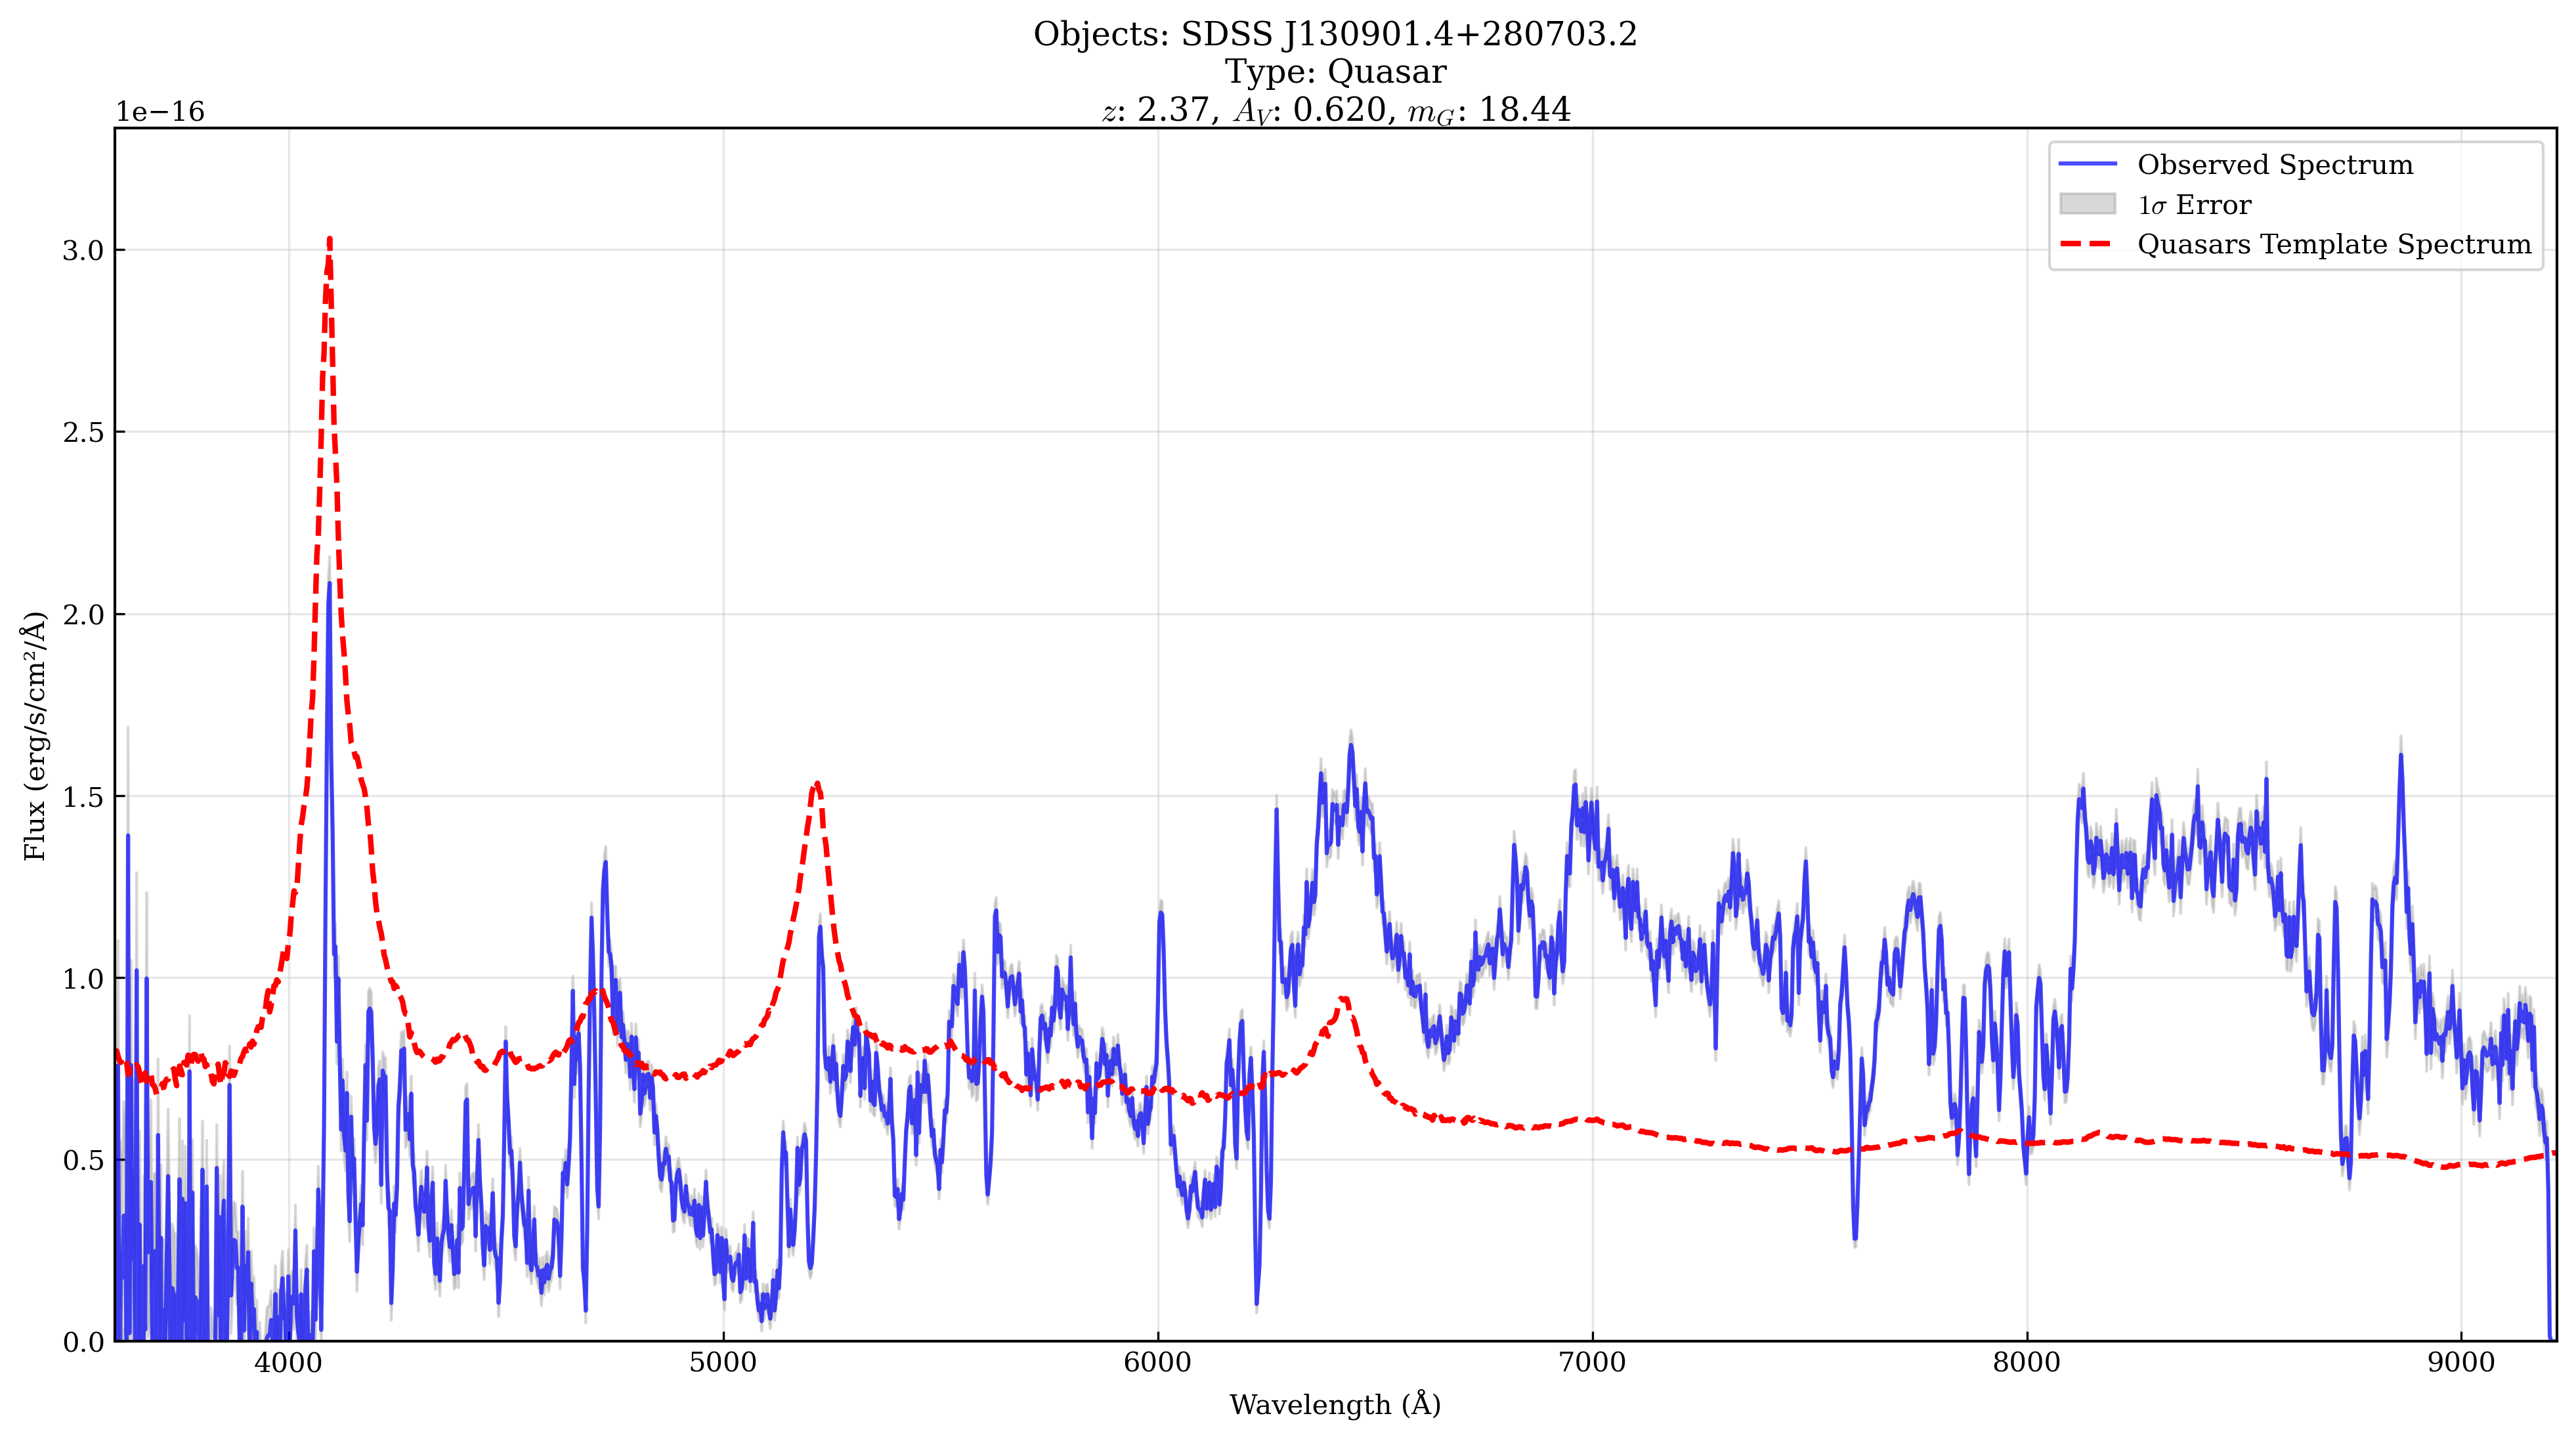
\includegraphics[width=\linewidth]{figs//raw/SDSS_J130901+280703.png}
    \end{subfigure} \\
    \begin{subfigure}[b]{0.45\textwidth}
        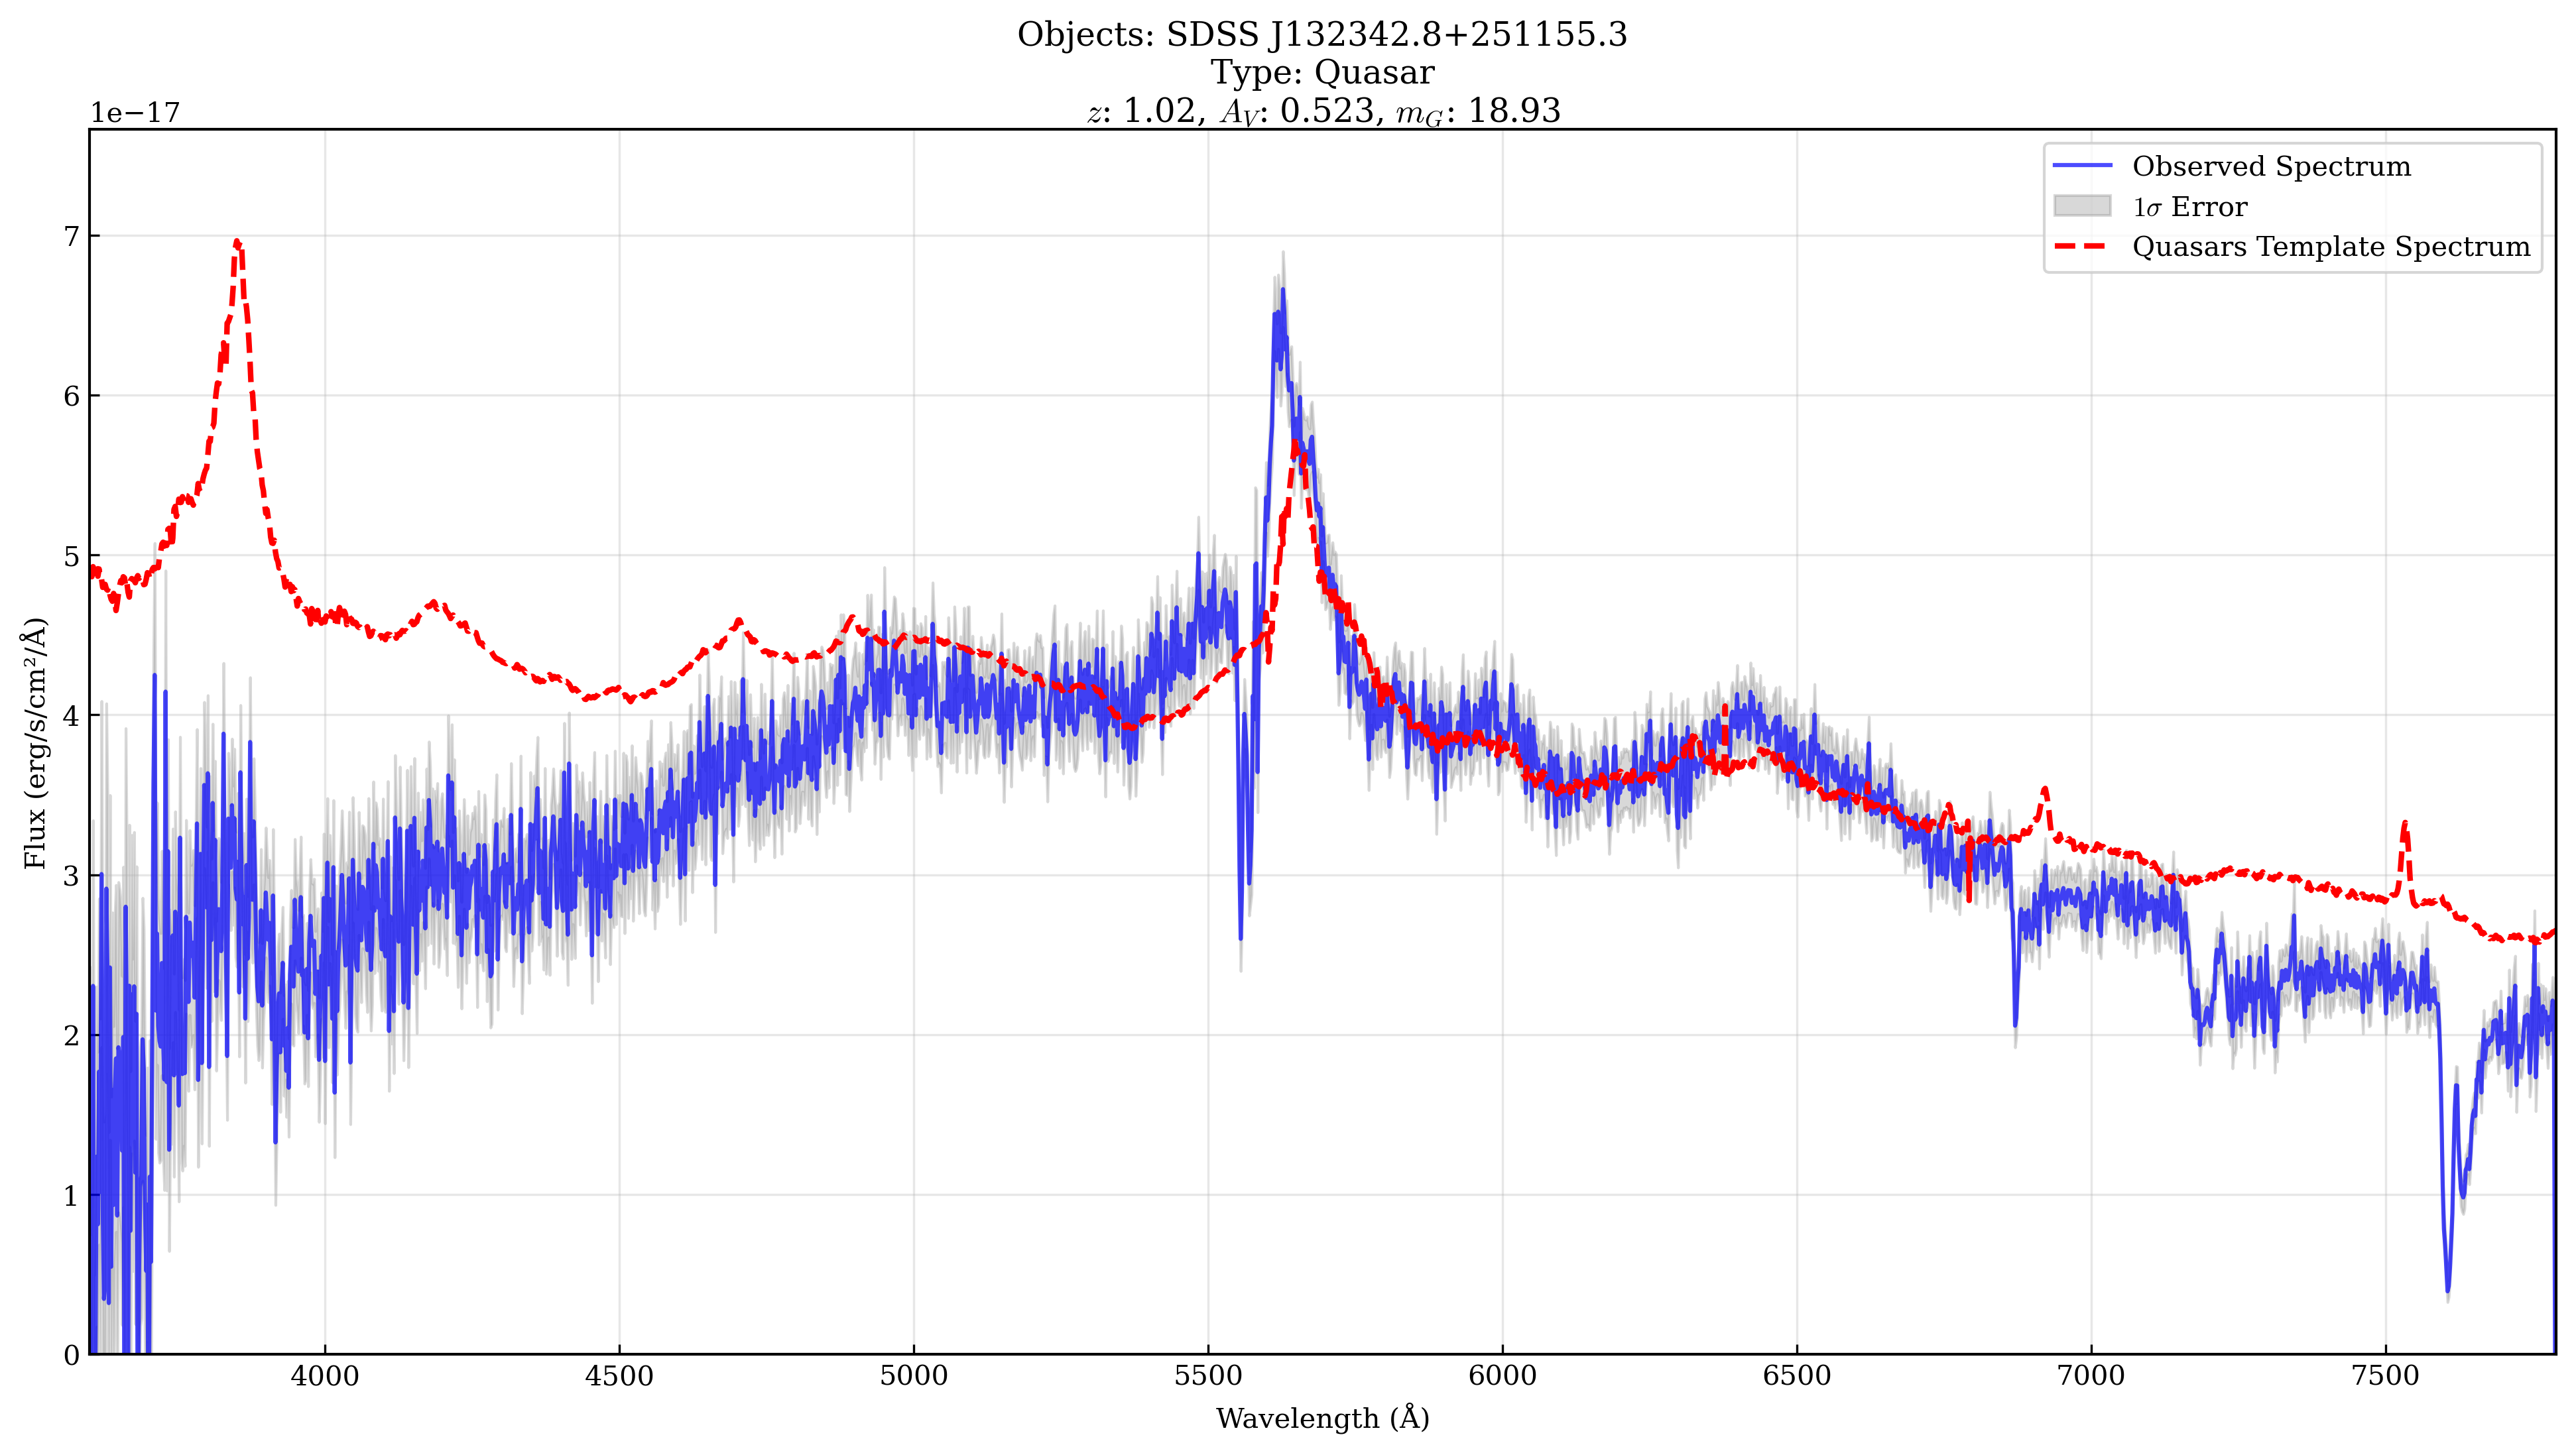
\includegraphics[width=\linewidth]{figs//raw/SDSS_J132342+251155.png}
    \end{subfigure}
    \begin{subfigure}[b]{0.45\textwidth}
        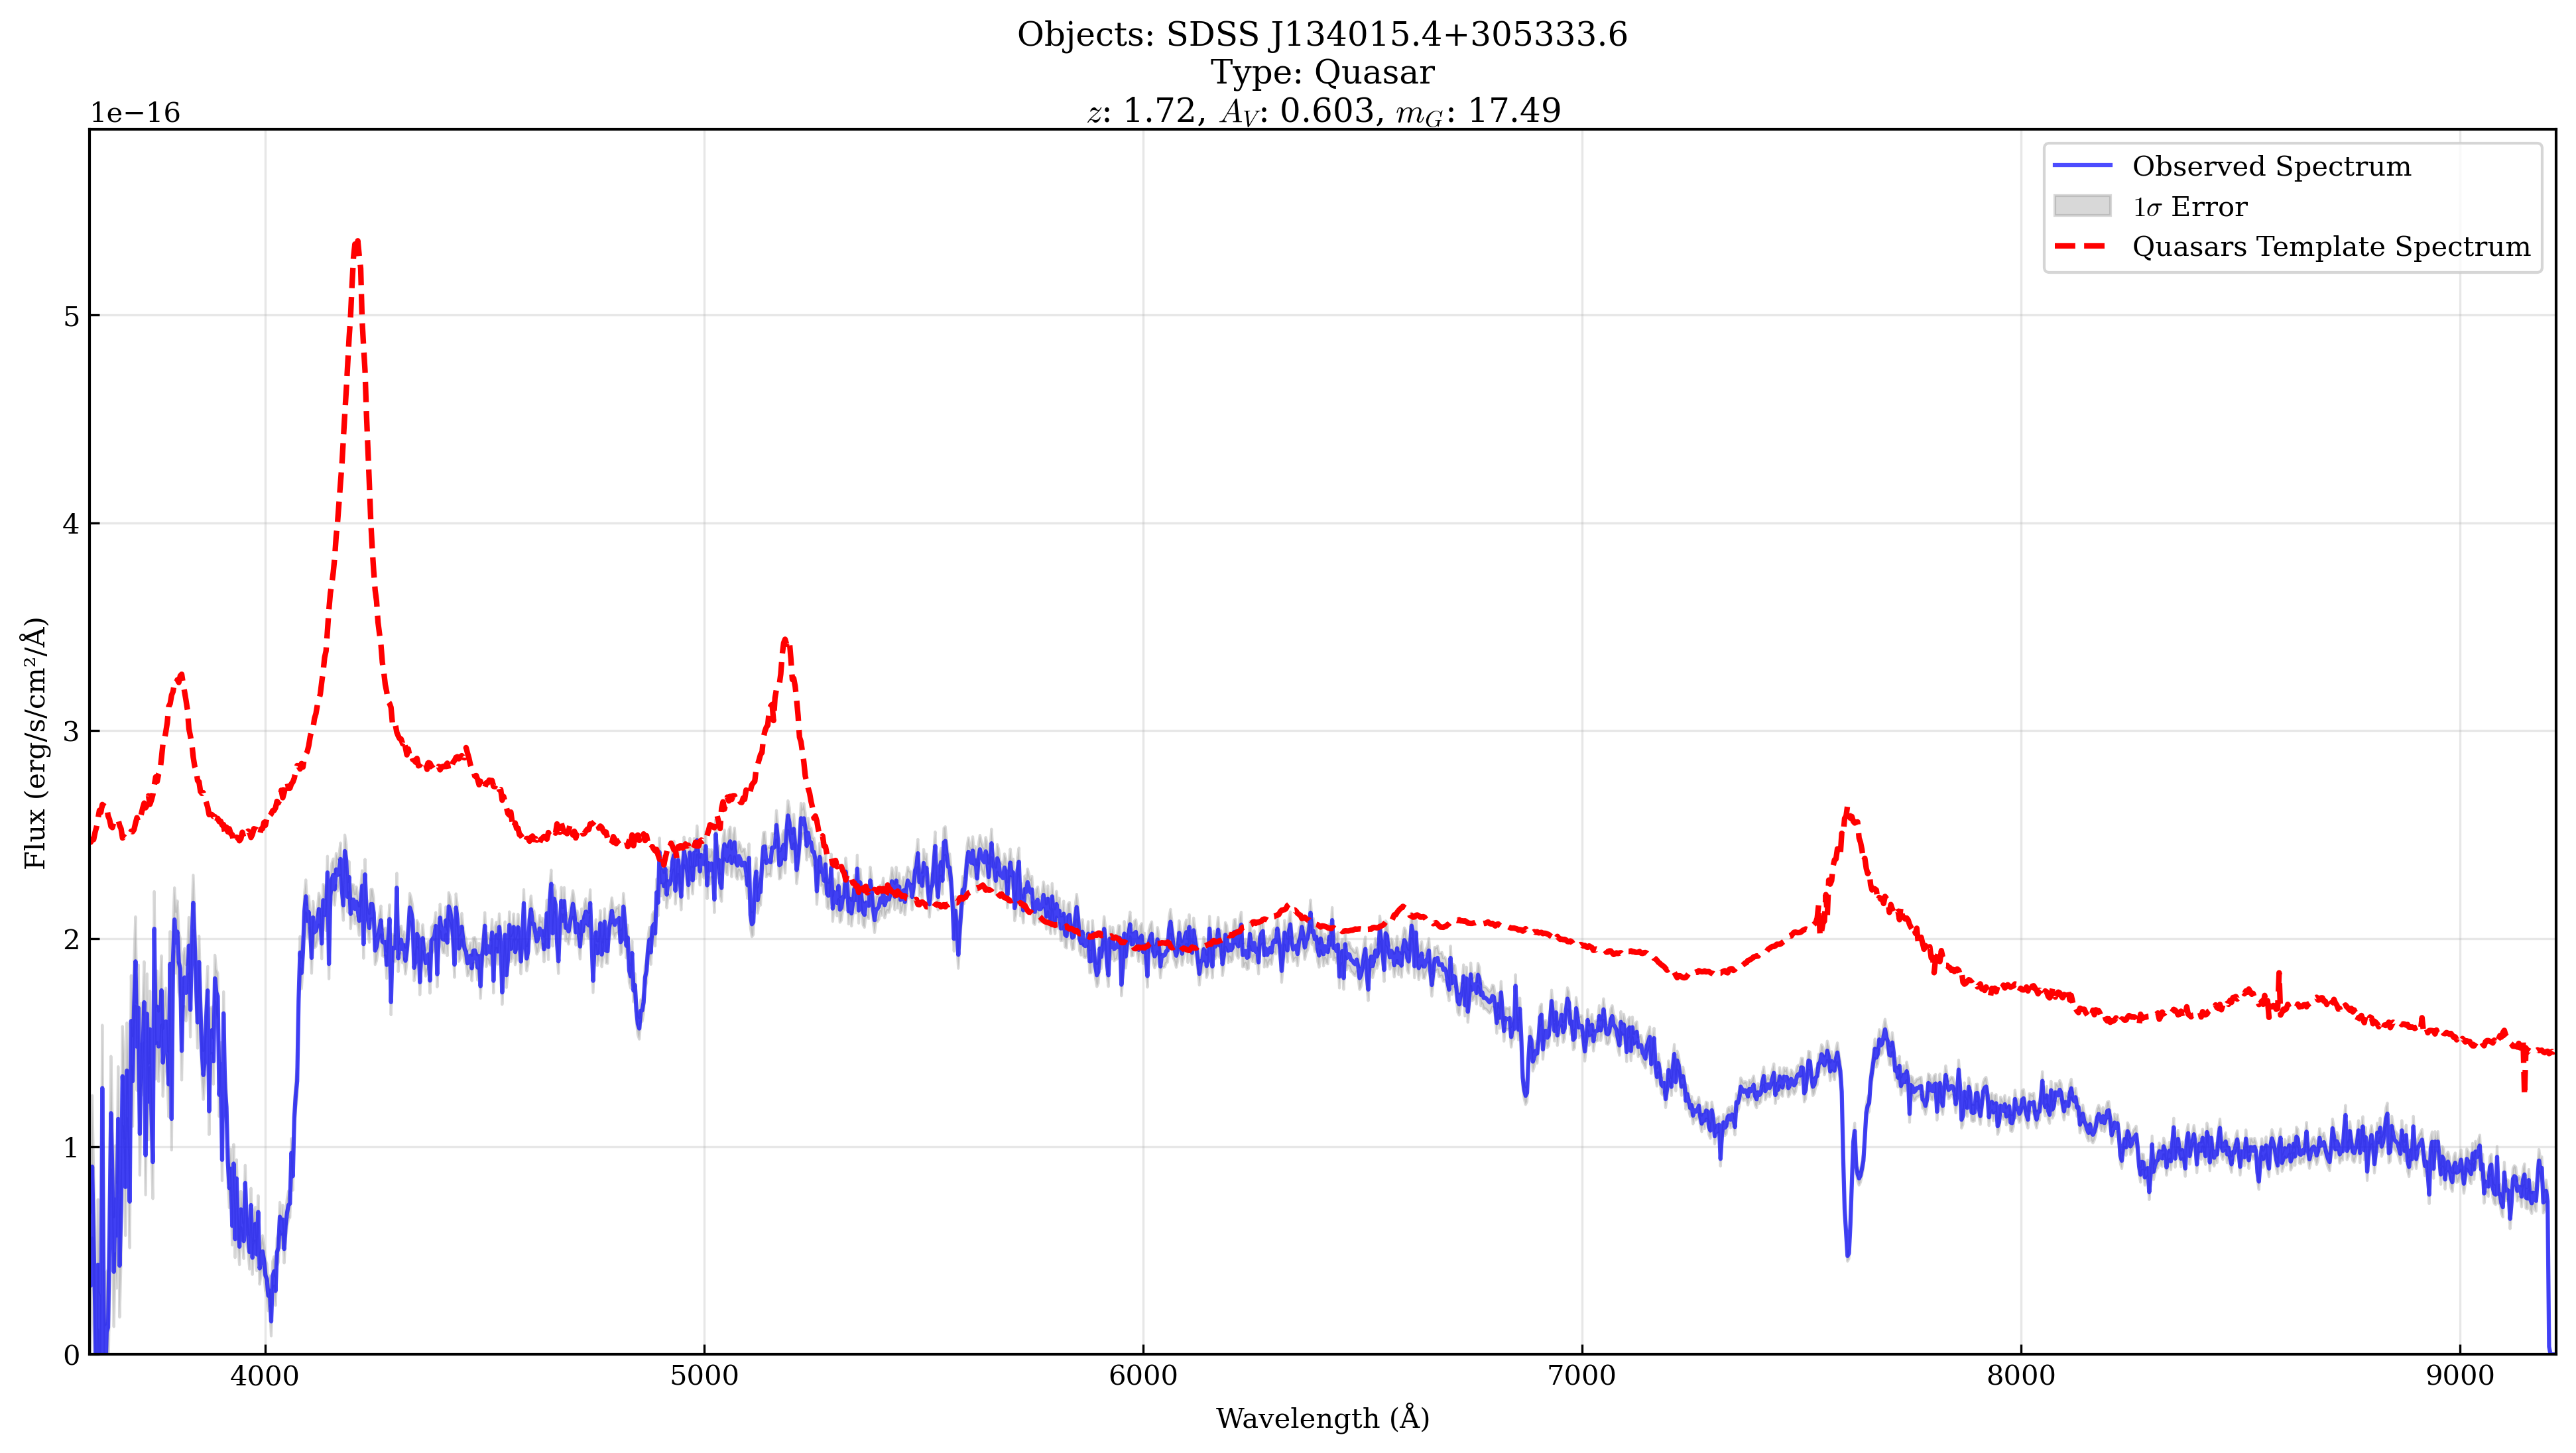
\includegraphics[width=\linewidth]{figs//raw/SDSS_J134015+305333.png}
    \end{subfigure} \\
    \begin{subfigure}[b]{0.45\textwidth}
        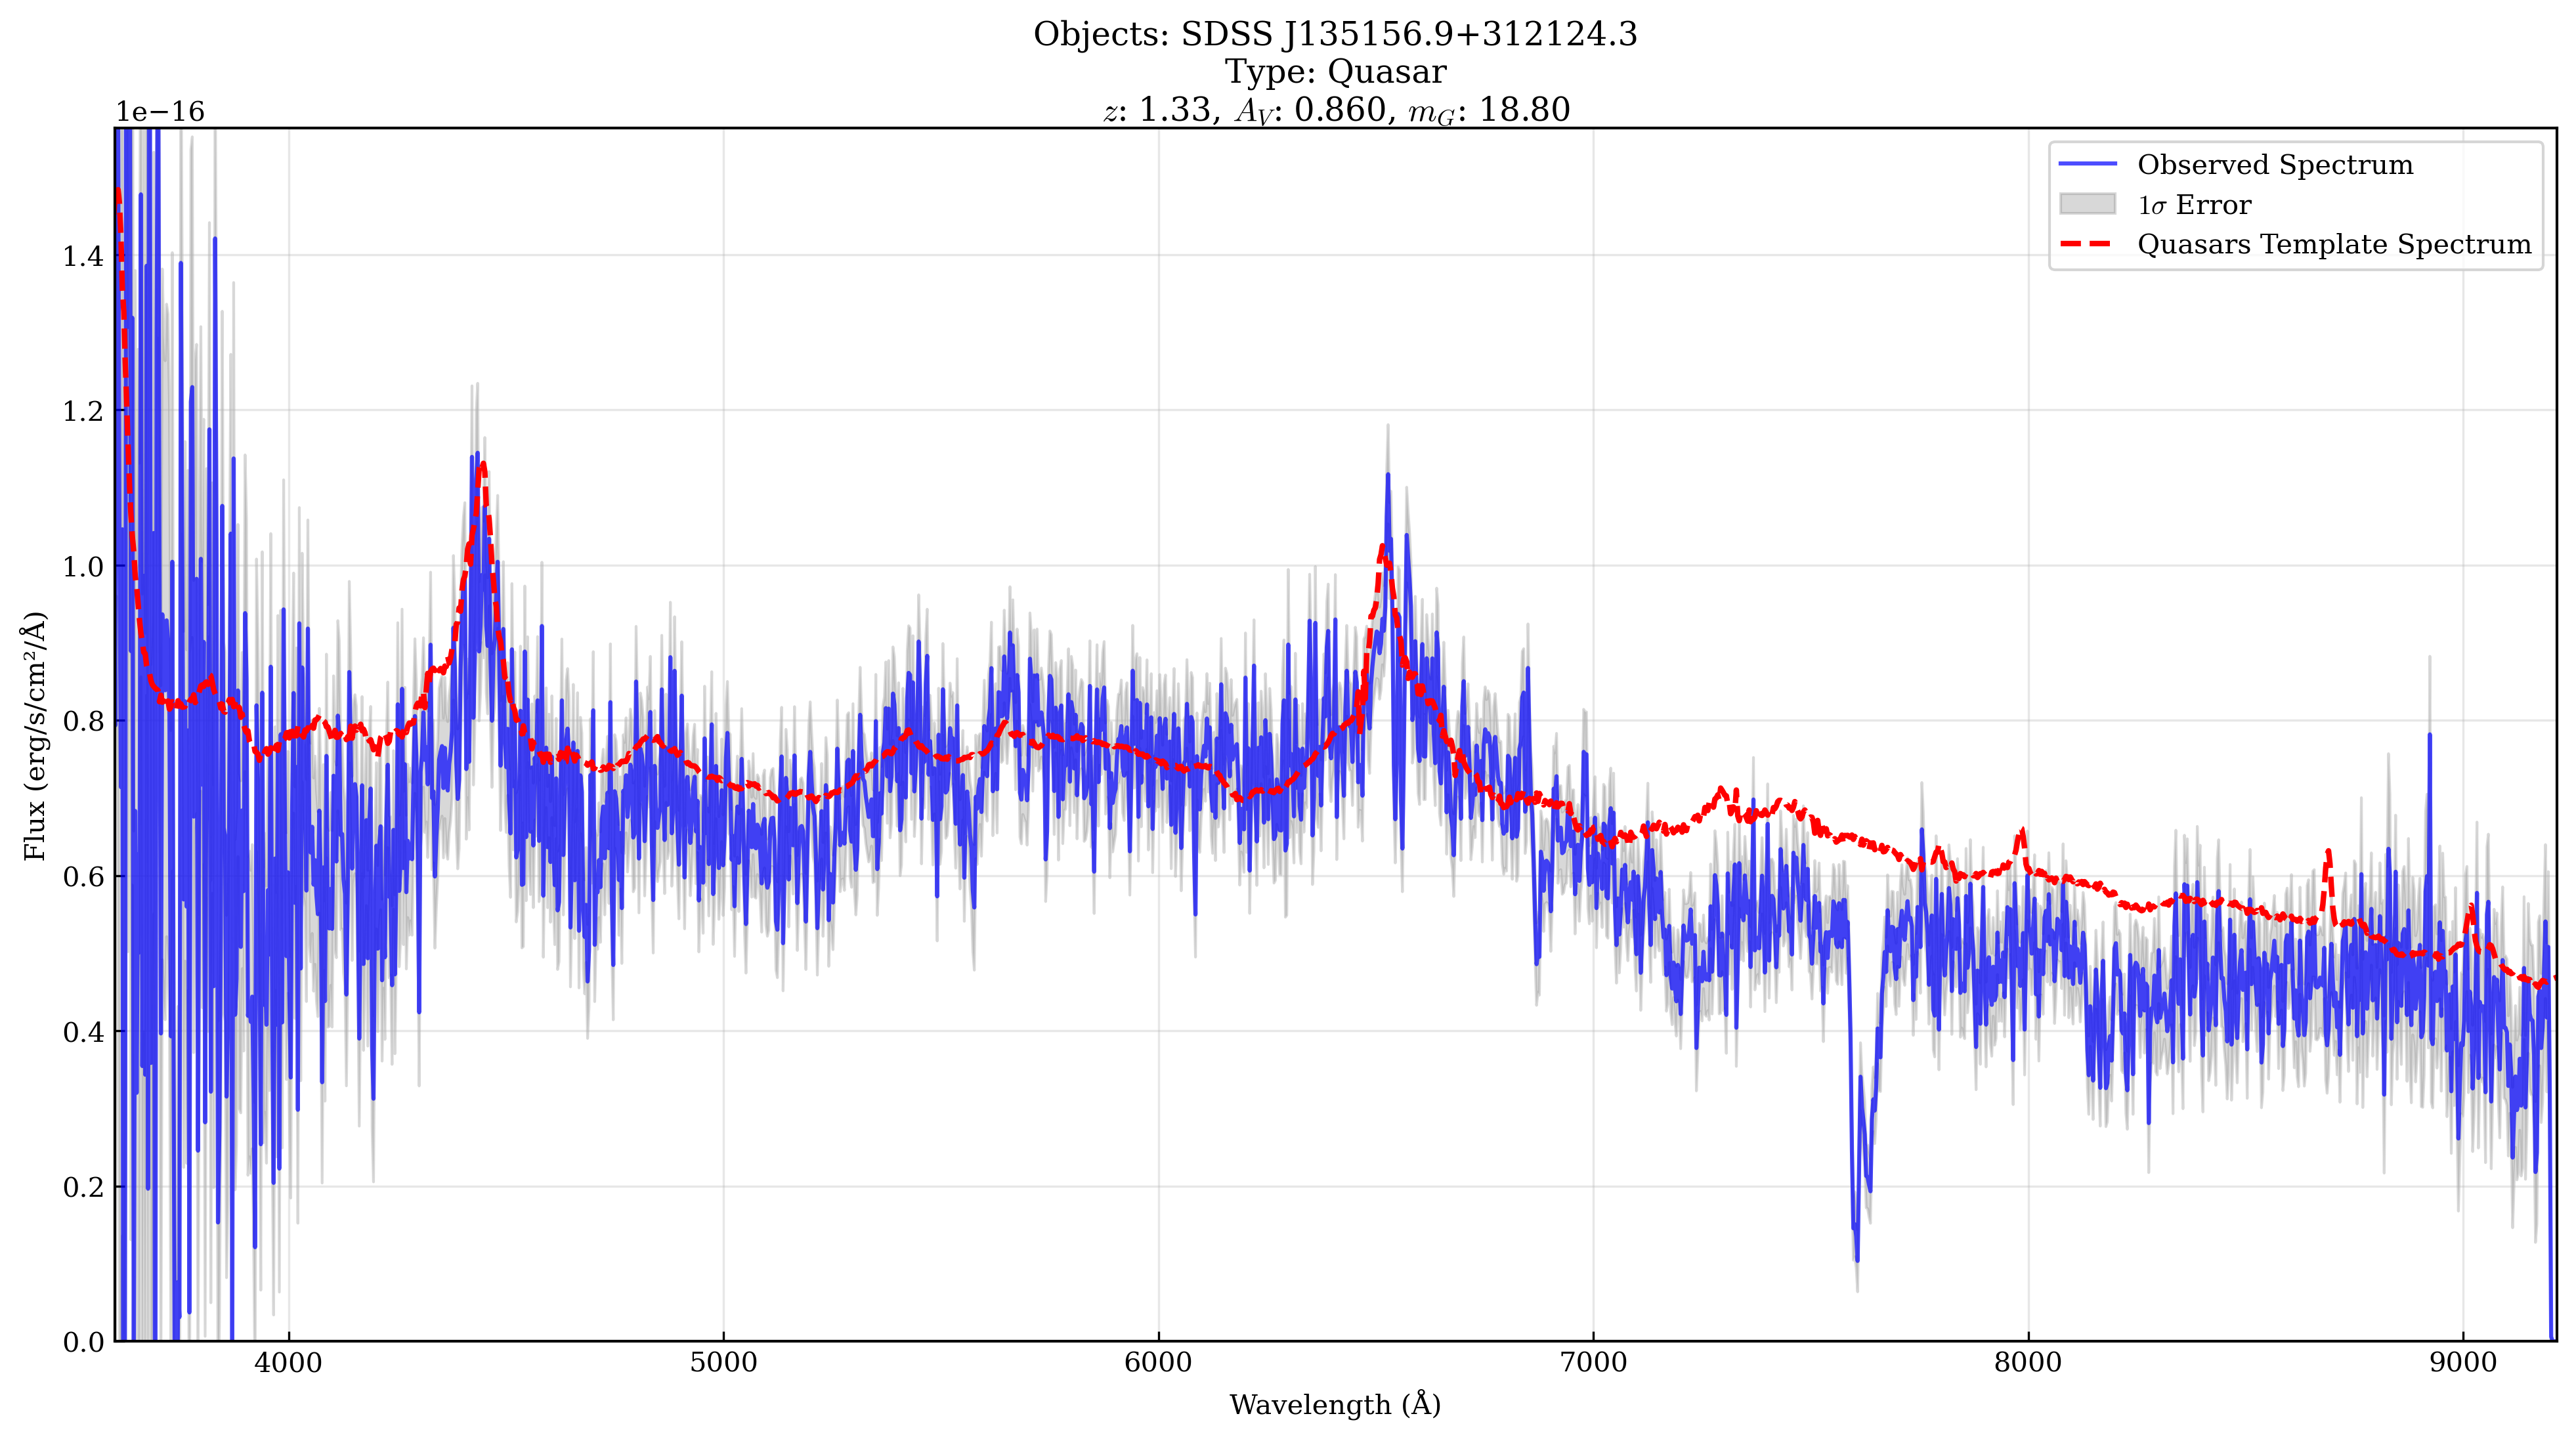
\includegraphics[width=\linewidth]{figs//raw/SDSS_J135156+312124.png}
    \end{subfigure}
    \begin{subfigure}[b]{0.45\textwidth}
        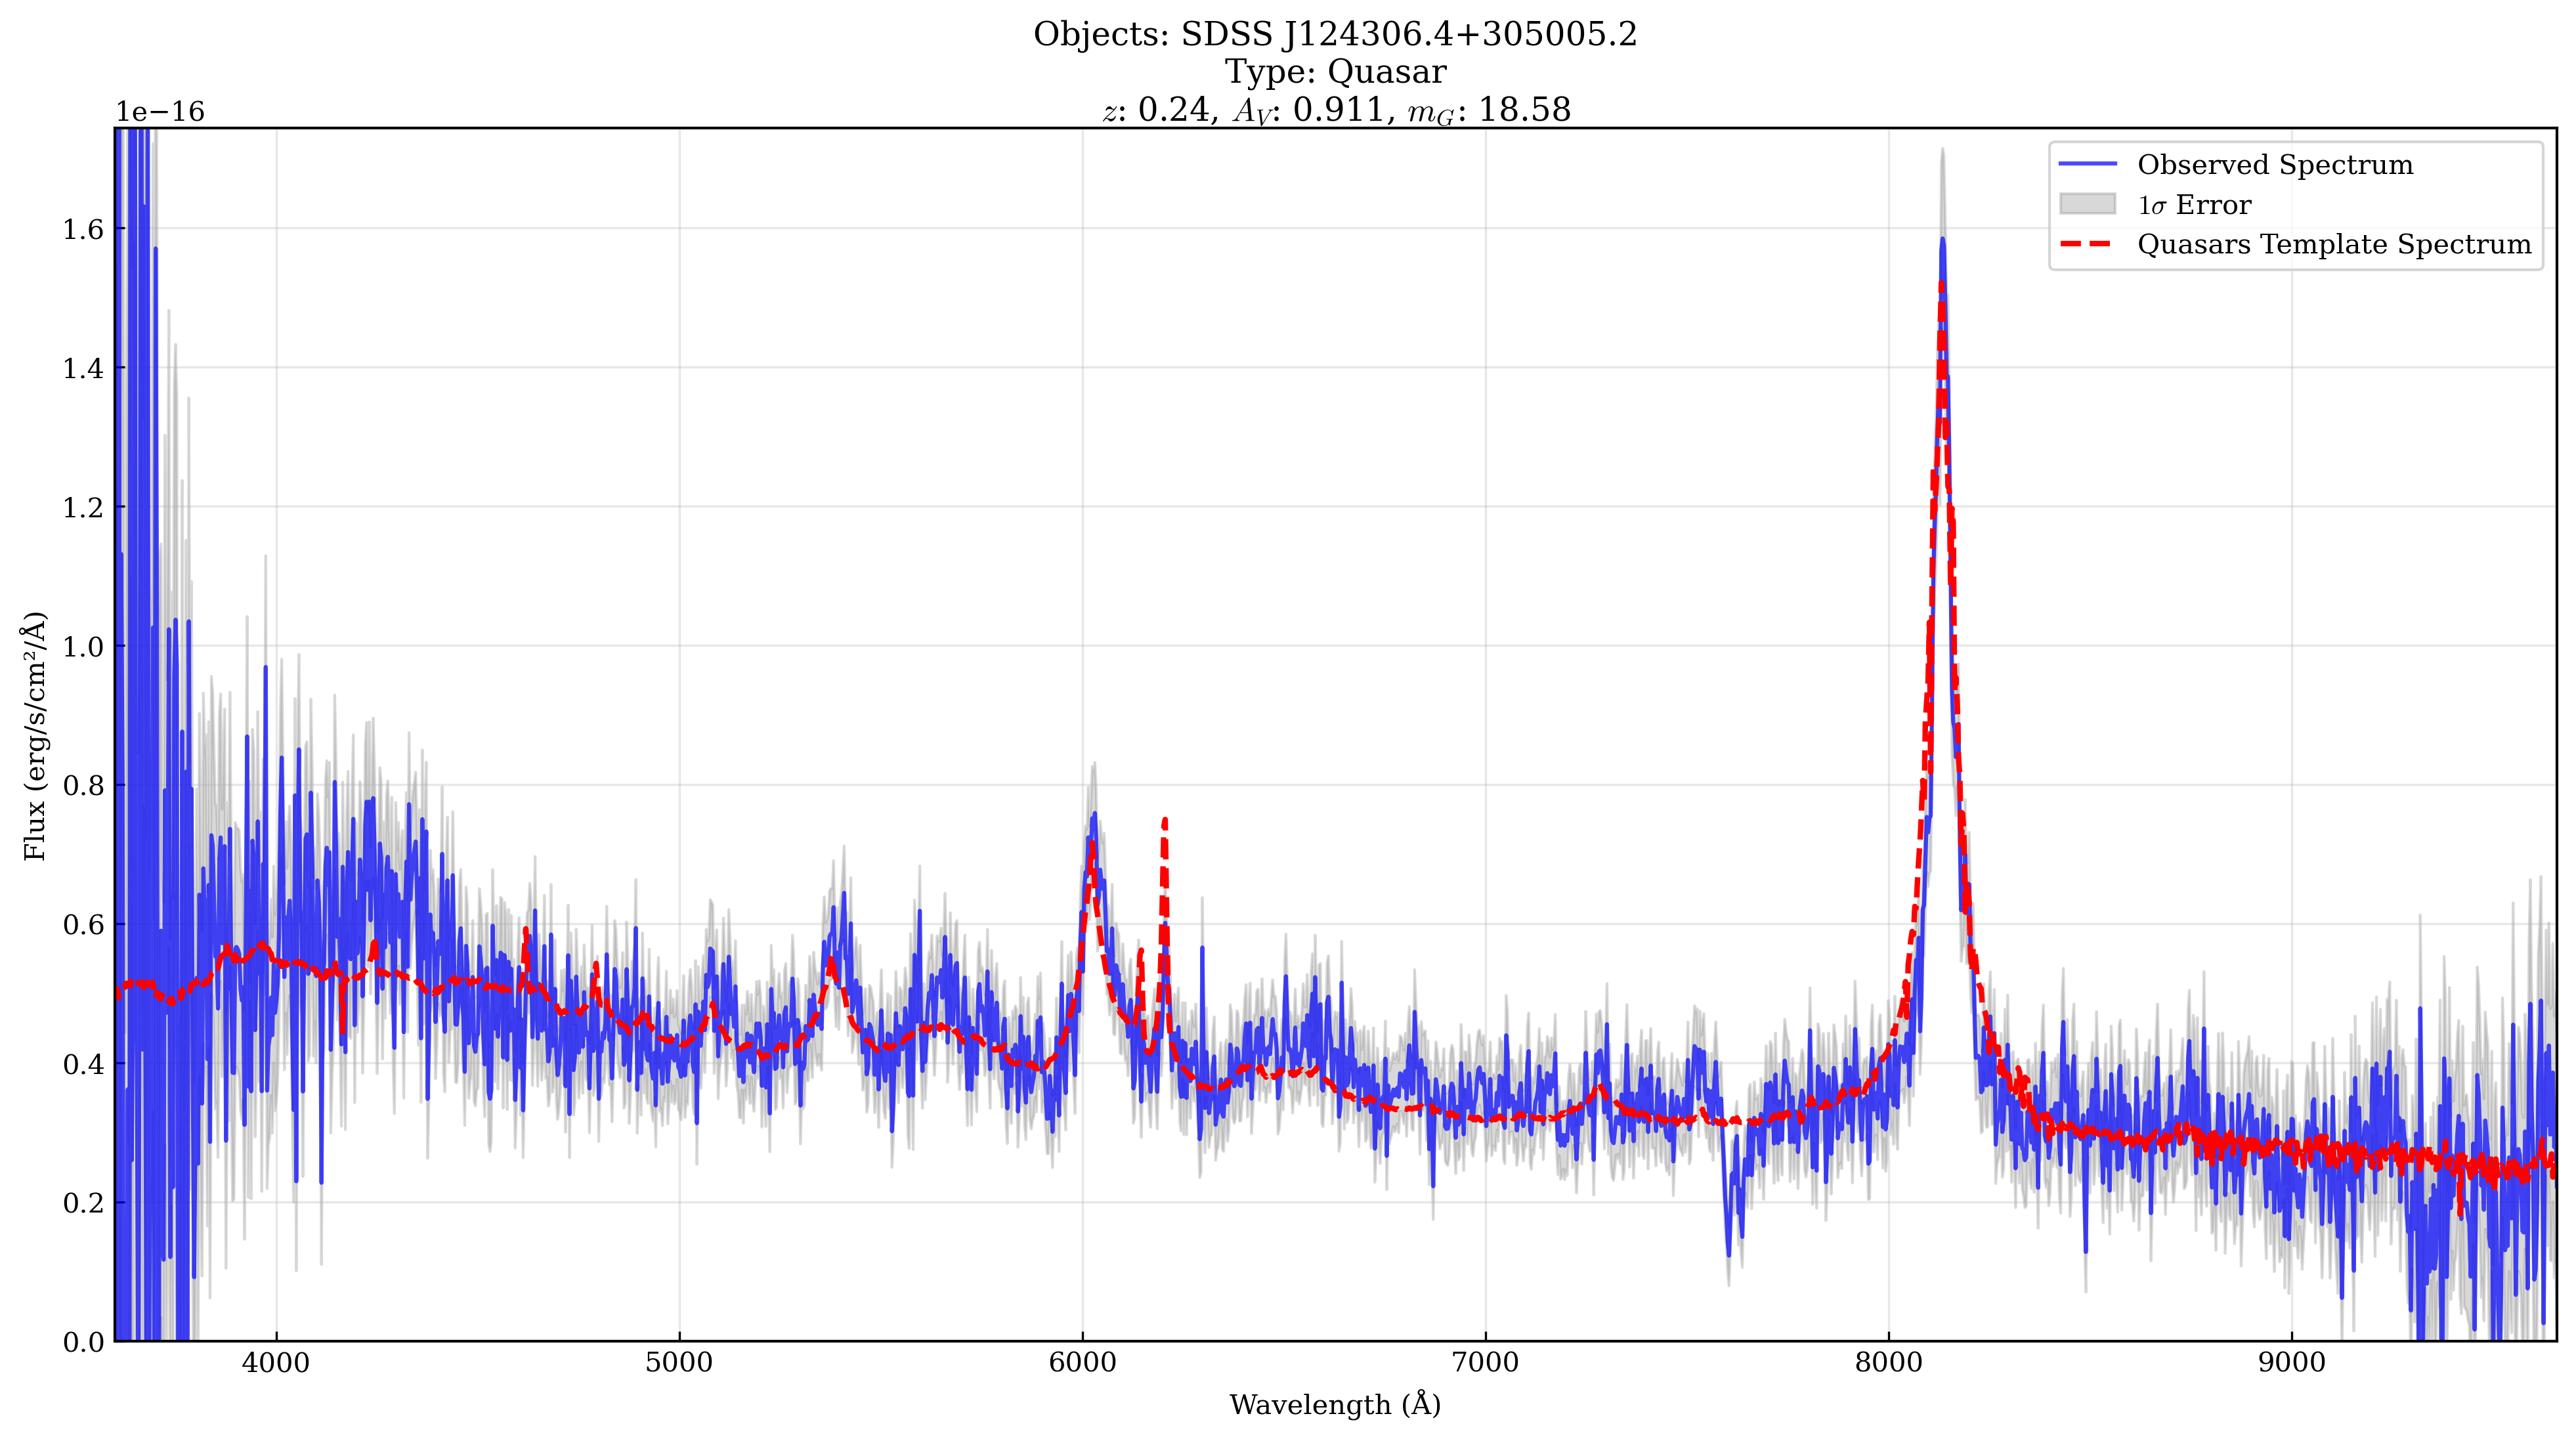
\includegraphics[width=\linewidth]{figs//raw/SDSS_J124306+305005.png}
    \end{subfigure} \\
    \begin{subfigure}[b]{0.45\textwidth}
        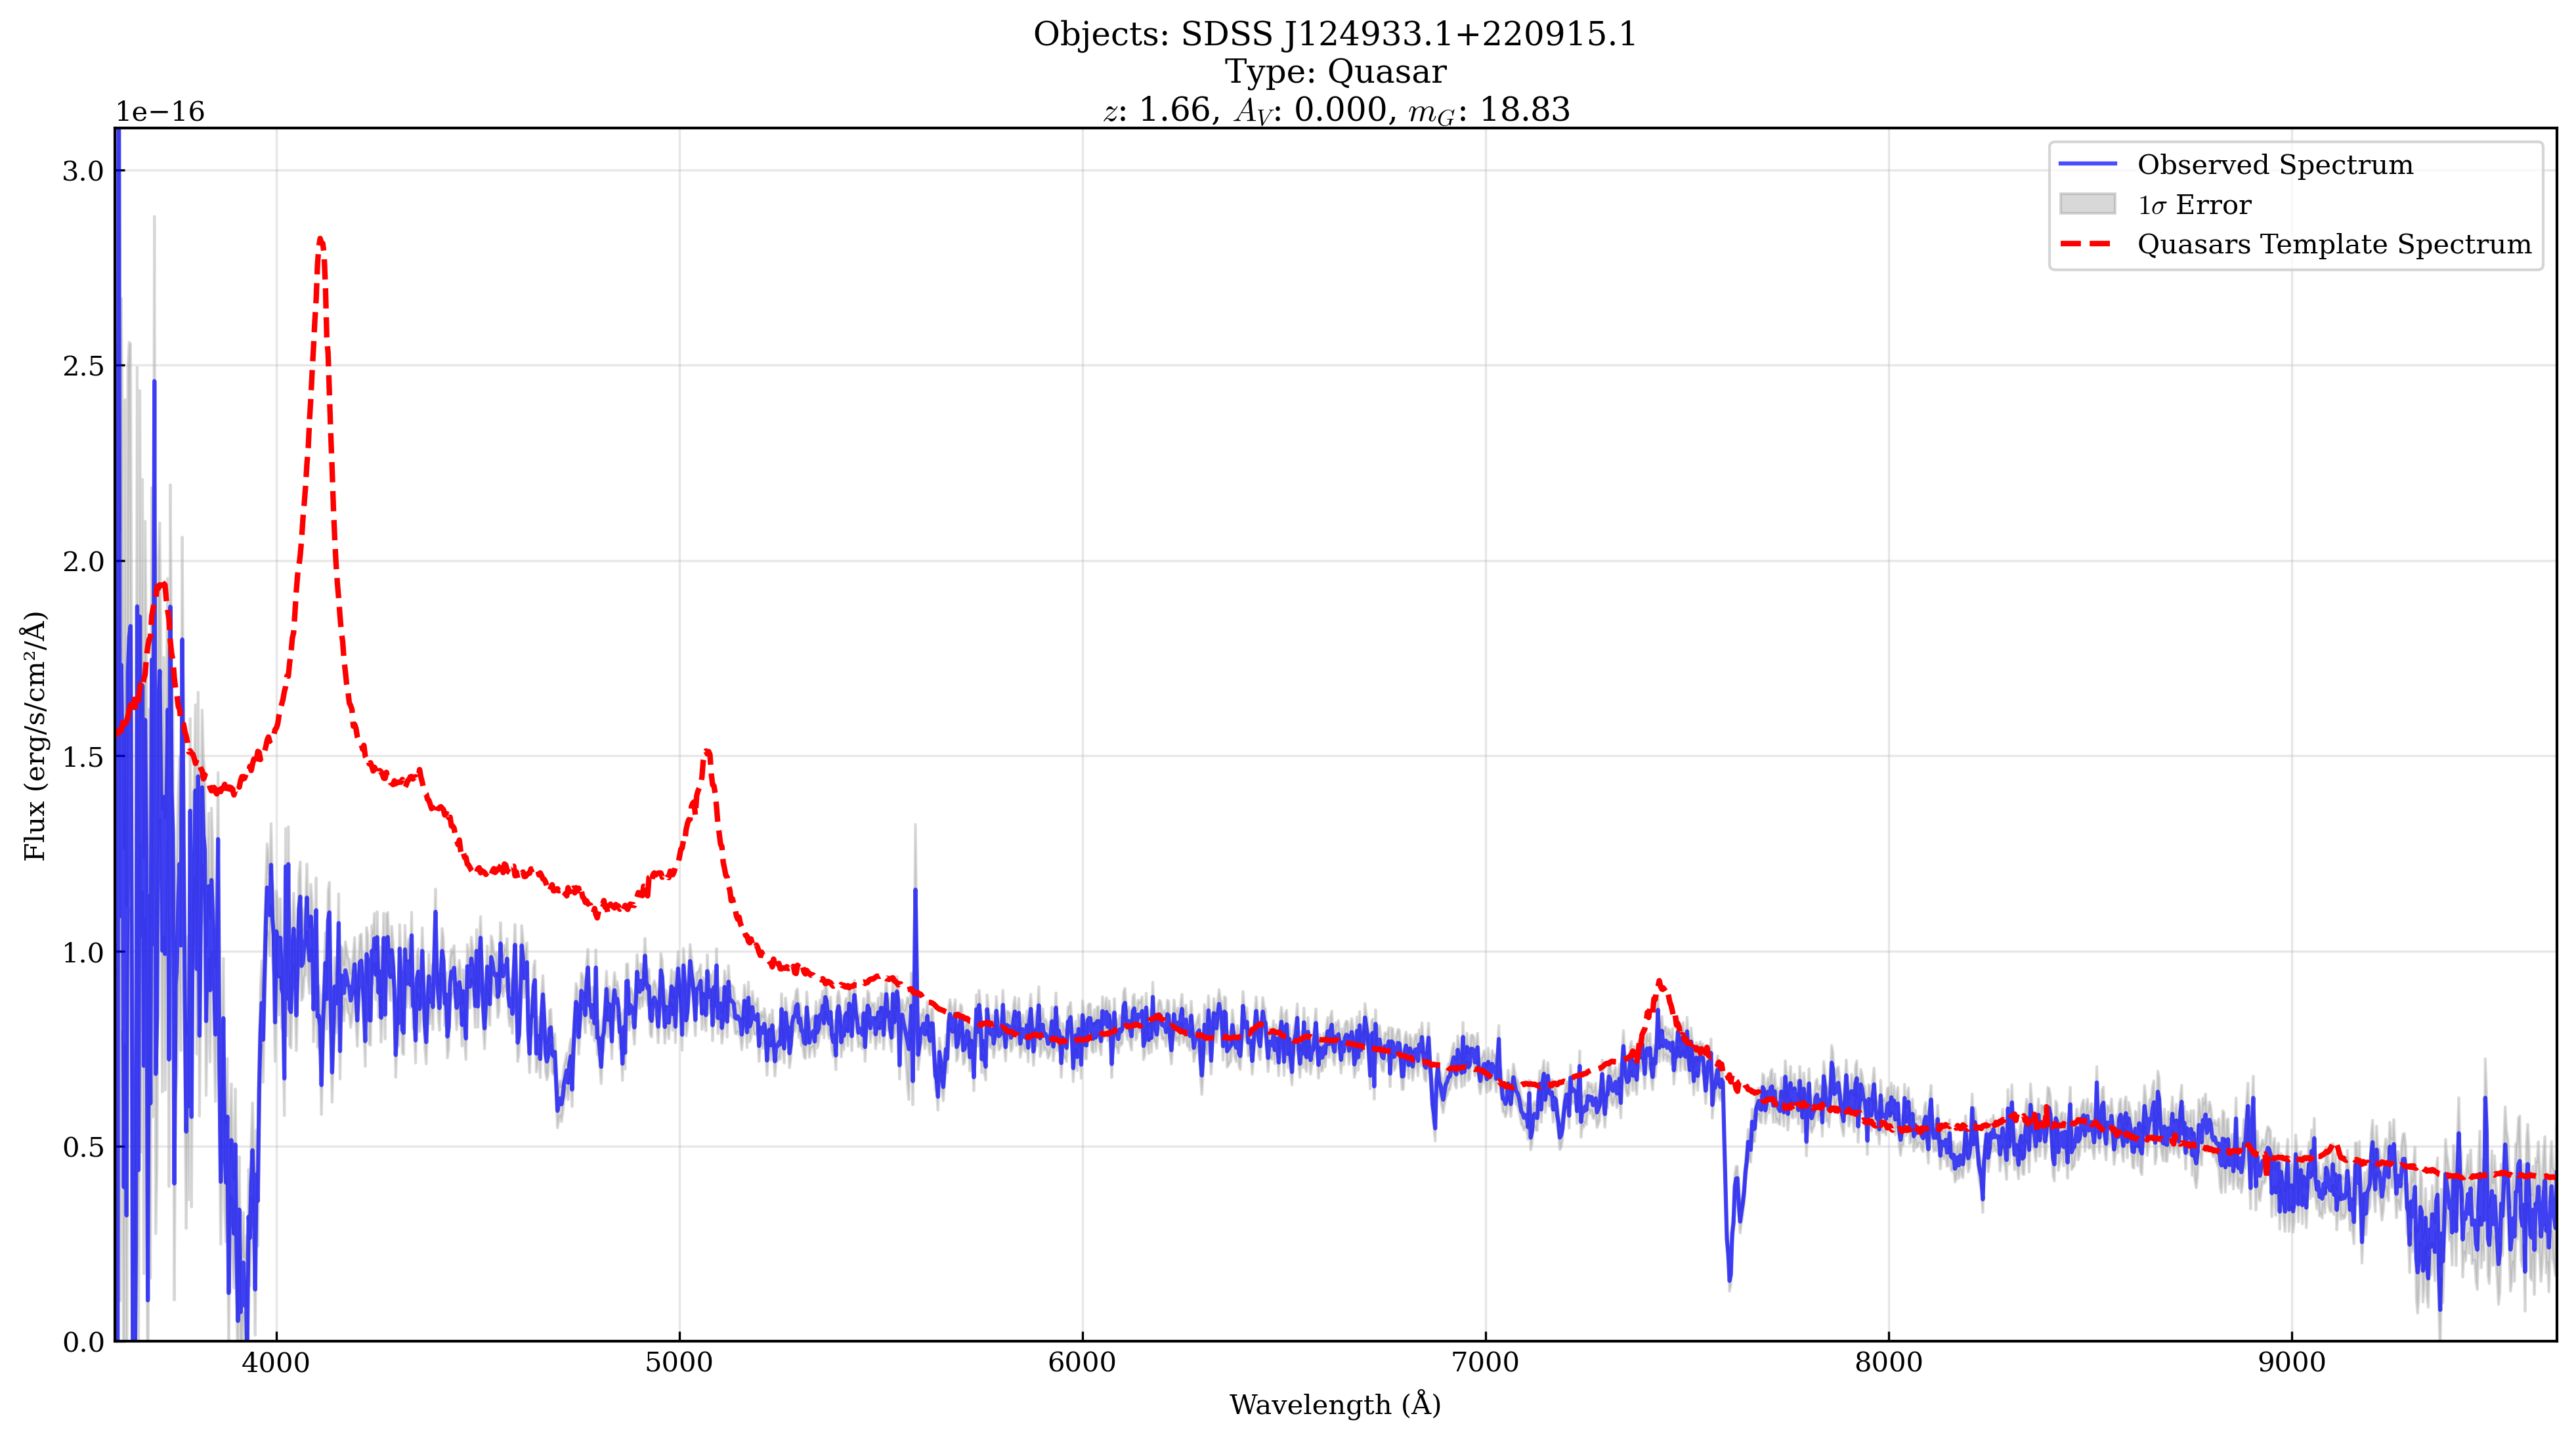
\includegraphics[width=\linewidth]{figs//raw/SDSS_J124933+220915.png}
    \end{subfigure}
    \begin{subfigure}[b]{0.45\textwidth}
        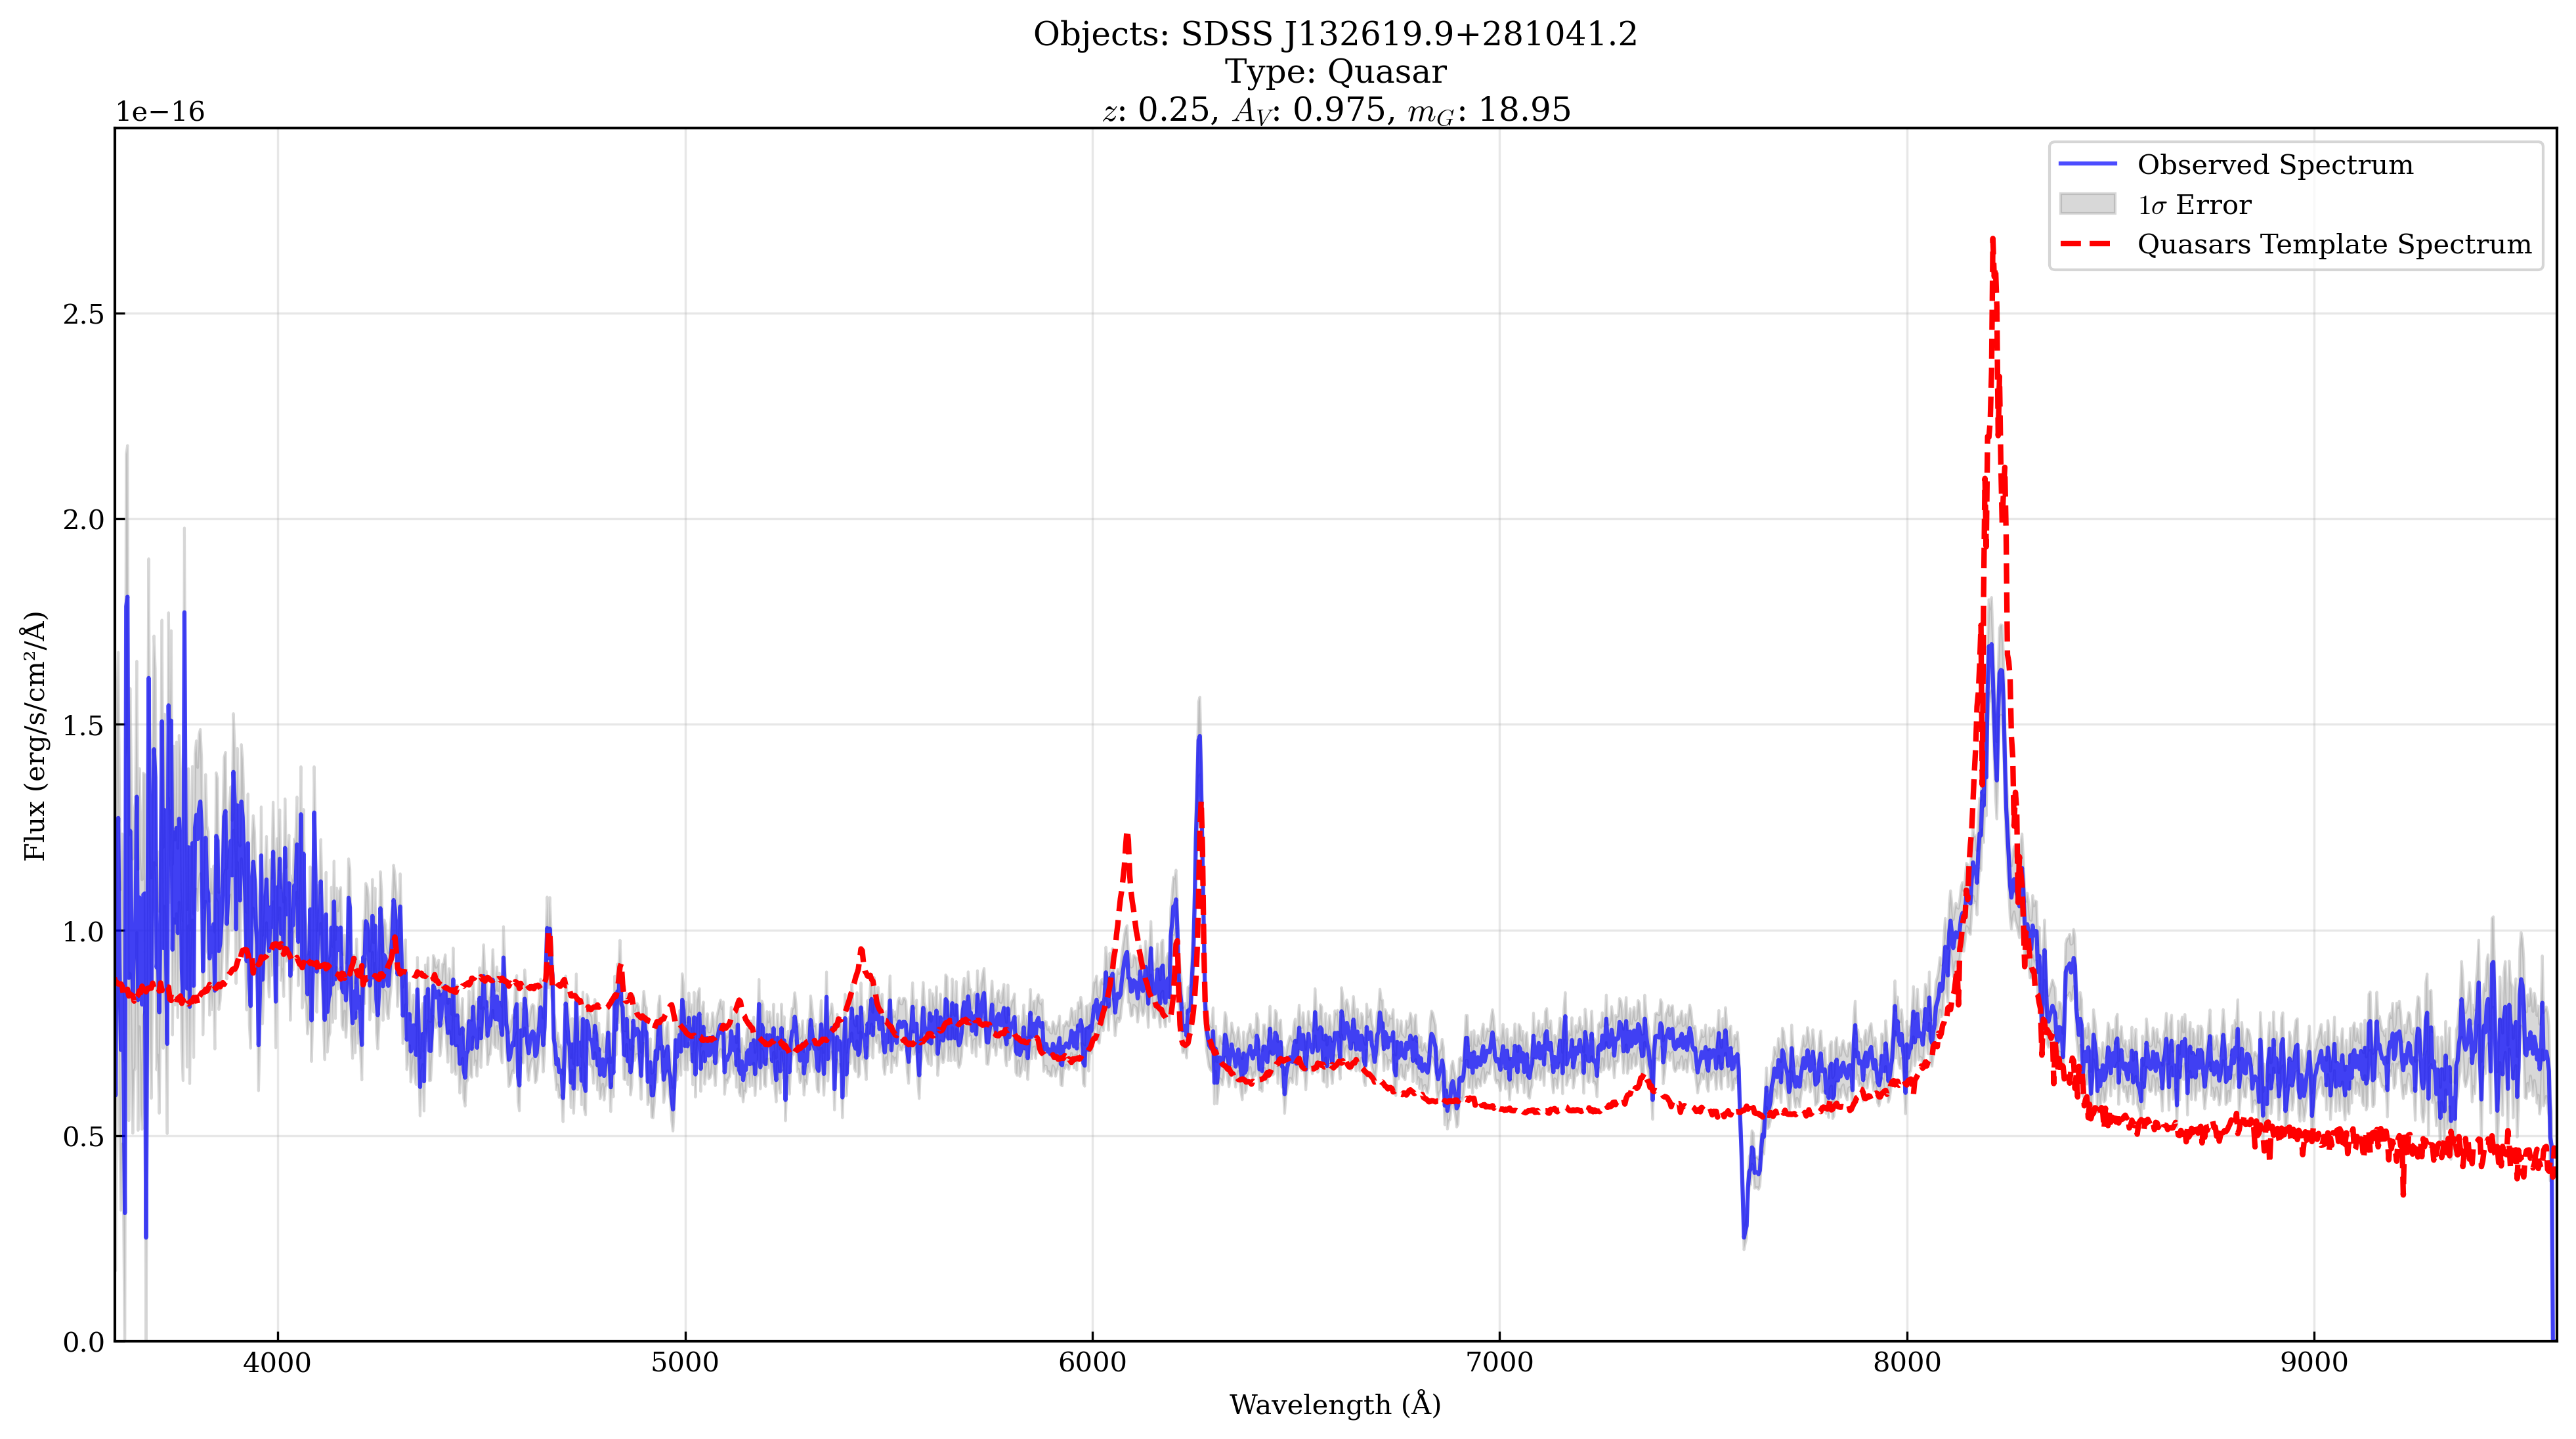
\includegraphics[width=\linewidth]{figs//raw/SDSS_J132619+281041.png}
    \end{subfigure} \\
    \begin{subfigure}[b]{0.45\textwidth}
        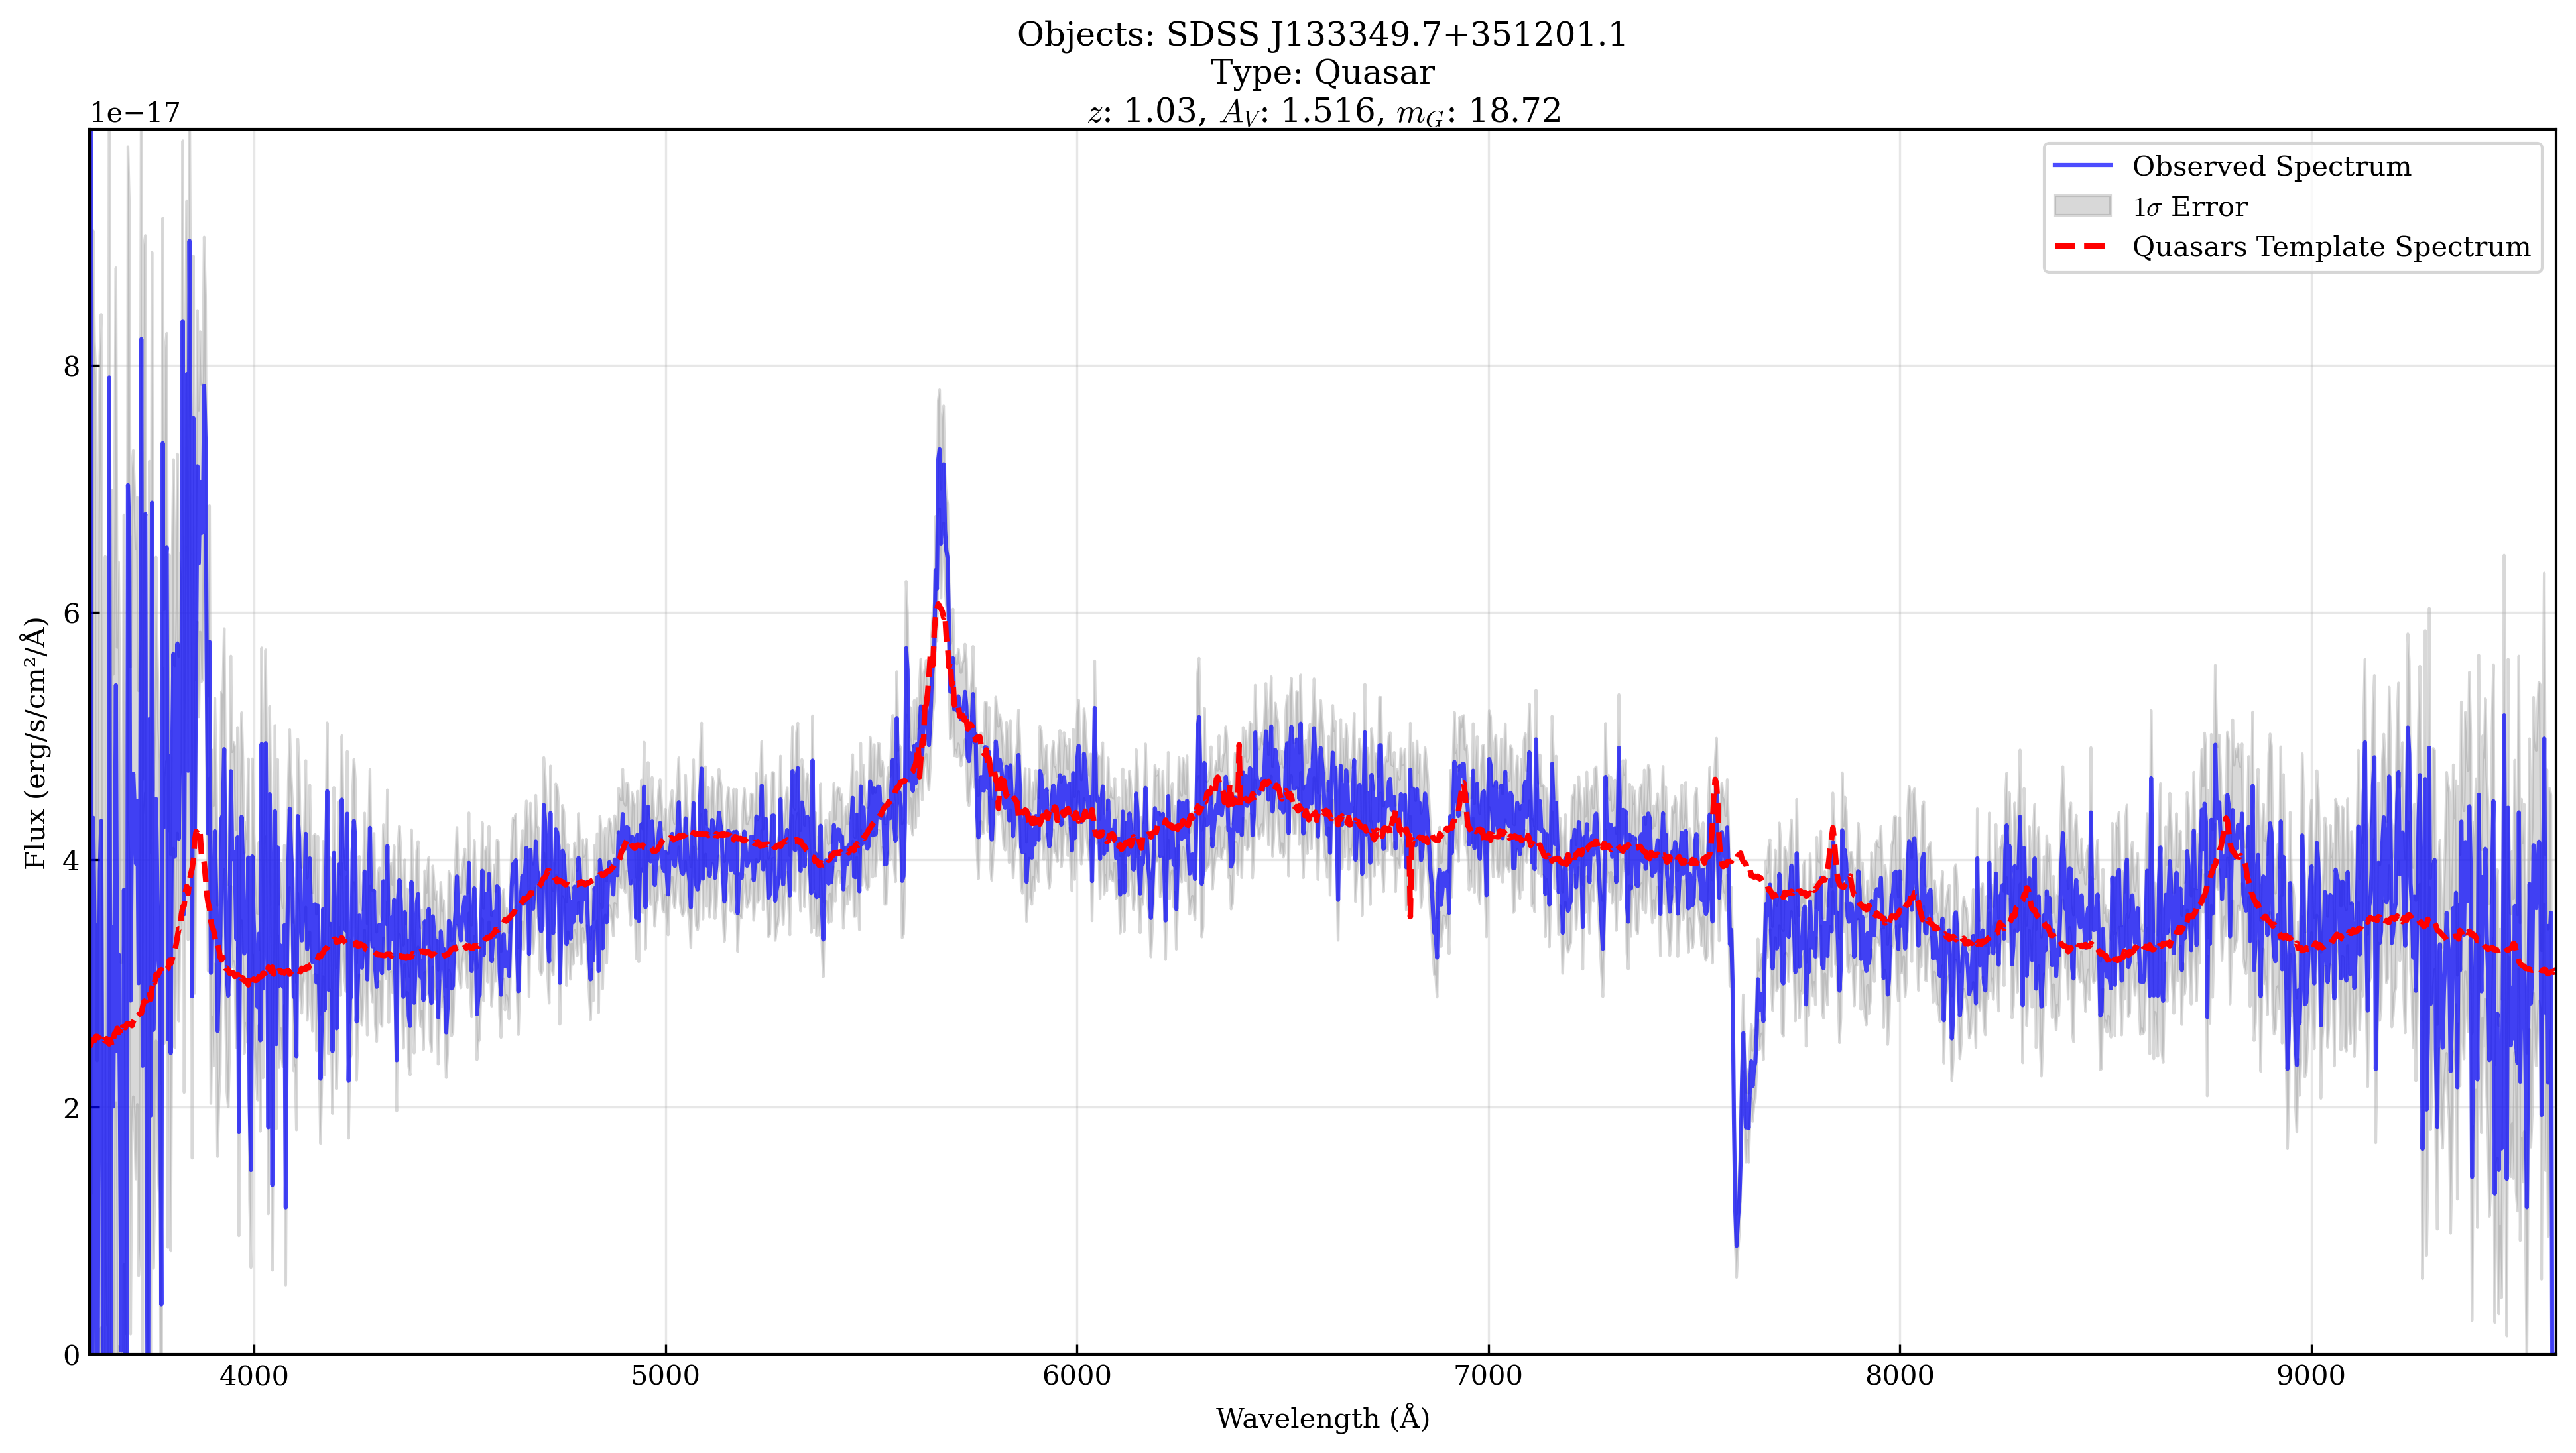
\includegraphics[width=\linewidth]{figs//raw/SDSS_J133349+351201.png}
    \end{subfigure}
    \begin{subfigure}[b]{0.45\textwidth}
        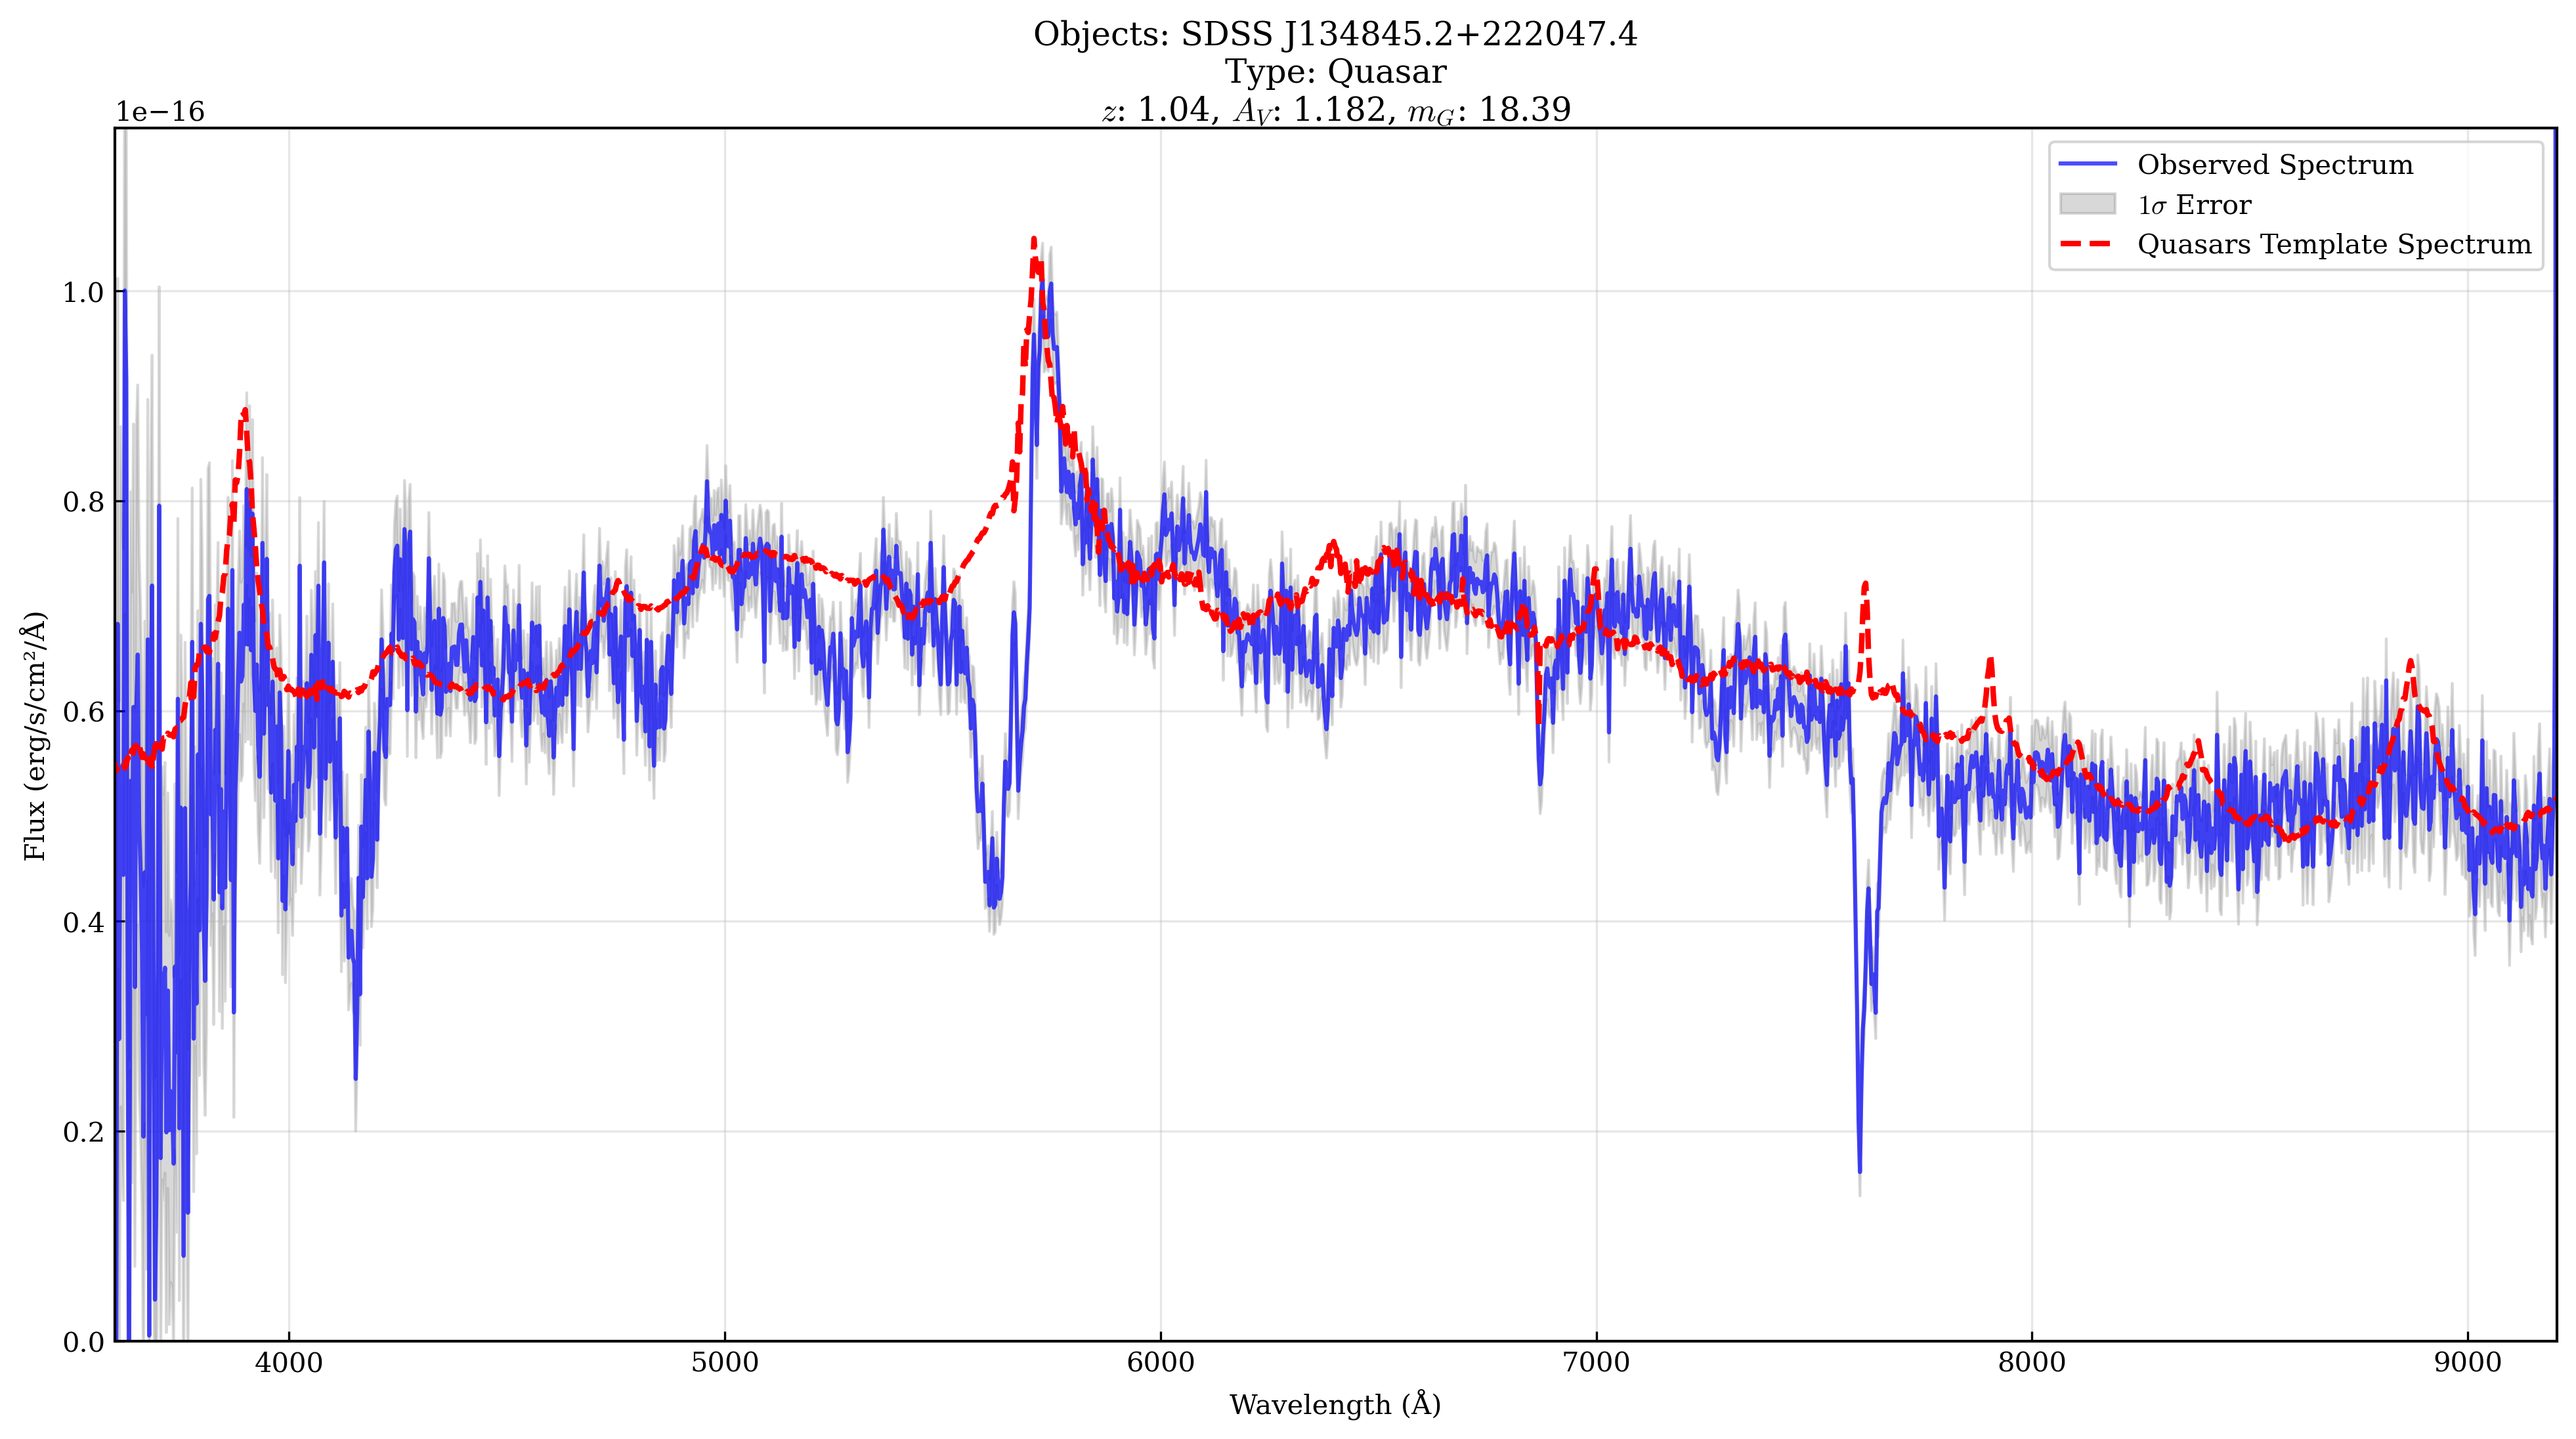
\includegraphics[width=\linewidth]{figs//raw/SDSS_J134845+222047.png}
    \end{subfigure}
    \caption{The targets with High Extinction $A_V>0.2$ \\ (Except \textbf{SDSS~J134010.6$+$273106.2})}
    \label{fig:high_av_qso}
\end{figure}

Figure~\ref{fig:high_av_qso} is a set of other high extinction ($A_V>0.2$) quasars. This set also contains some BAL quasars (Such as \textbf{SDSS~J134015.4$+$305333.6}, \textbf{SDSS~J124933.1$+$220915.1}, \textbf{SDSS~J134845.2$+$222047.4}), because they are around by dust. \textbf{SDSS~J130901.4$+$280703.2} is another unusual quasar, which may contains not only one AGN.

\subsection{Stars}

We also find two interesting targets marked as stars in our observations -- \textbf{SDSS~J131310.5$+$232833.9} and \textbf{SDSS~J132035.7$+$340814.6}.

\paragraph{SDSS~J131310.5$+$232833.9}  \\

This is a blue horizontal branch star(BHB). From \texttt{NutMaat}, it is marked as B9.5 type star. We also use $\chi^2$ test to match MILES library from \citep{sanchez-blazquezMediumresolutionIsaacNewton2006}, and the result is Figure~\ref{fig:bhb_miles}. High effective temperatures ($T_{\text{eff}}$) and low metallicity ([Fe/H]) make it is a BHB star in high probability.
\begin{figure}[htbp]
    \centering
    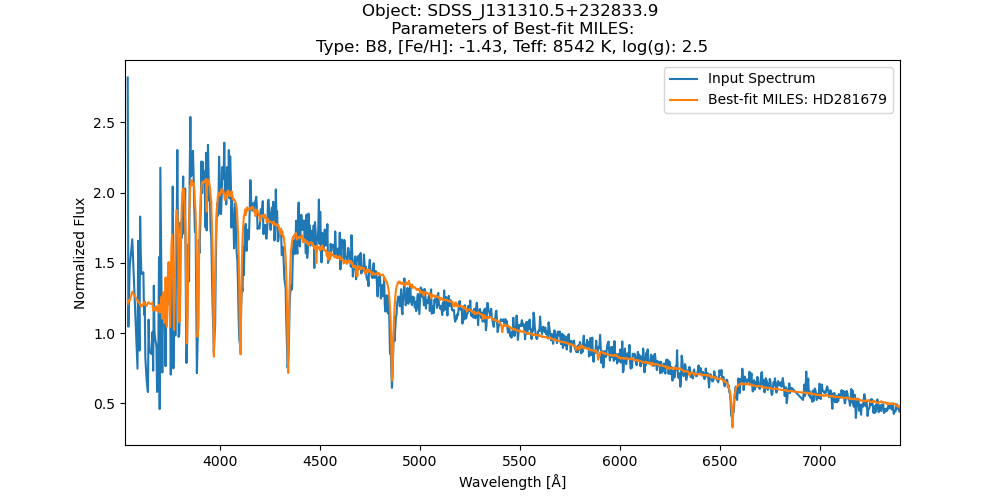
\includegraphics[width=0.9\linewidth]{figs//res/miles_fit_SDSS_J131310+232833.png}
    \caption{The target \textbf{SDSS~J131310.5$+$232833.9} with the Best Fitted Template in MILES}
    \label{fig:bhb_miles}
\end{figure}

BHB stars are low-mass, metal-poor stars in advanced stages of stellar evolution. Following the helium flash at the tip of the Red Giant Branch (RGB), these stars enter a stable phase sustained by core helium fusion and hydrogen shell burning \citep{hoyleEvolutionTypeII1955, roseHeliumShellBurningStars1966}. On the Hertzsprung-Russell (HR) diagram, they are situated to the upper left of the main sequence, characterized by high effective temperatures ($T_{\text{eff}} > 7000\text{ K}$‬) and relatively low surface gravities \citep{catelanHorizontalBranchStars2009}. 

Their absolute magnitudes remain relatively constant across a broad range of colours, and they predominantly populate ancient globular clusters and the Galactic halo. As a result, BHB stars are extensively utilized as excellent standard candles for tracing the chemical and dynamical evolutionary history of the Galactic halo \citep{xueMilkyWaysCircular2008}.

So we could estimate the distance of this star. We could assume the absolute magnitude in Gaia G-Band of this star is $M_G=0.6$ \citep{barbosaSDSSGaiaViewColor2022}. And the visual magnitude of this star is $m_G=18.96$. Using the distance modulus , we could get luminosity distance of this star: \[D_{L}=10^{\frac {(m_G-M_G)}{5}+1} \approx 4.7 \mathrm{kpc}\] Which means this is a star which is far from Milky Way's plate.

\paragraph{SDSS~J132035.7$+$340814.6} \\

This target is a star cluster located in near galaxy at $z=0.023$. Figure~\ref{fig:star_cluster} is the spectrum of it we observed. 
\begin{figure}[htbp]
    \centering
    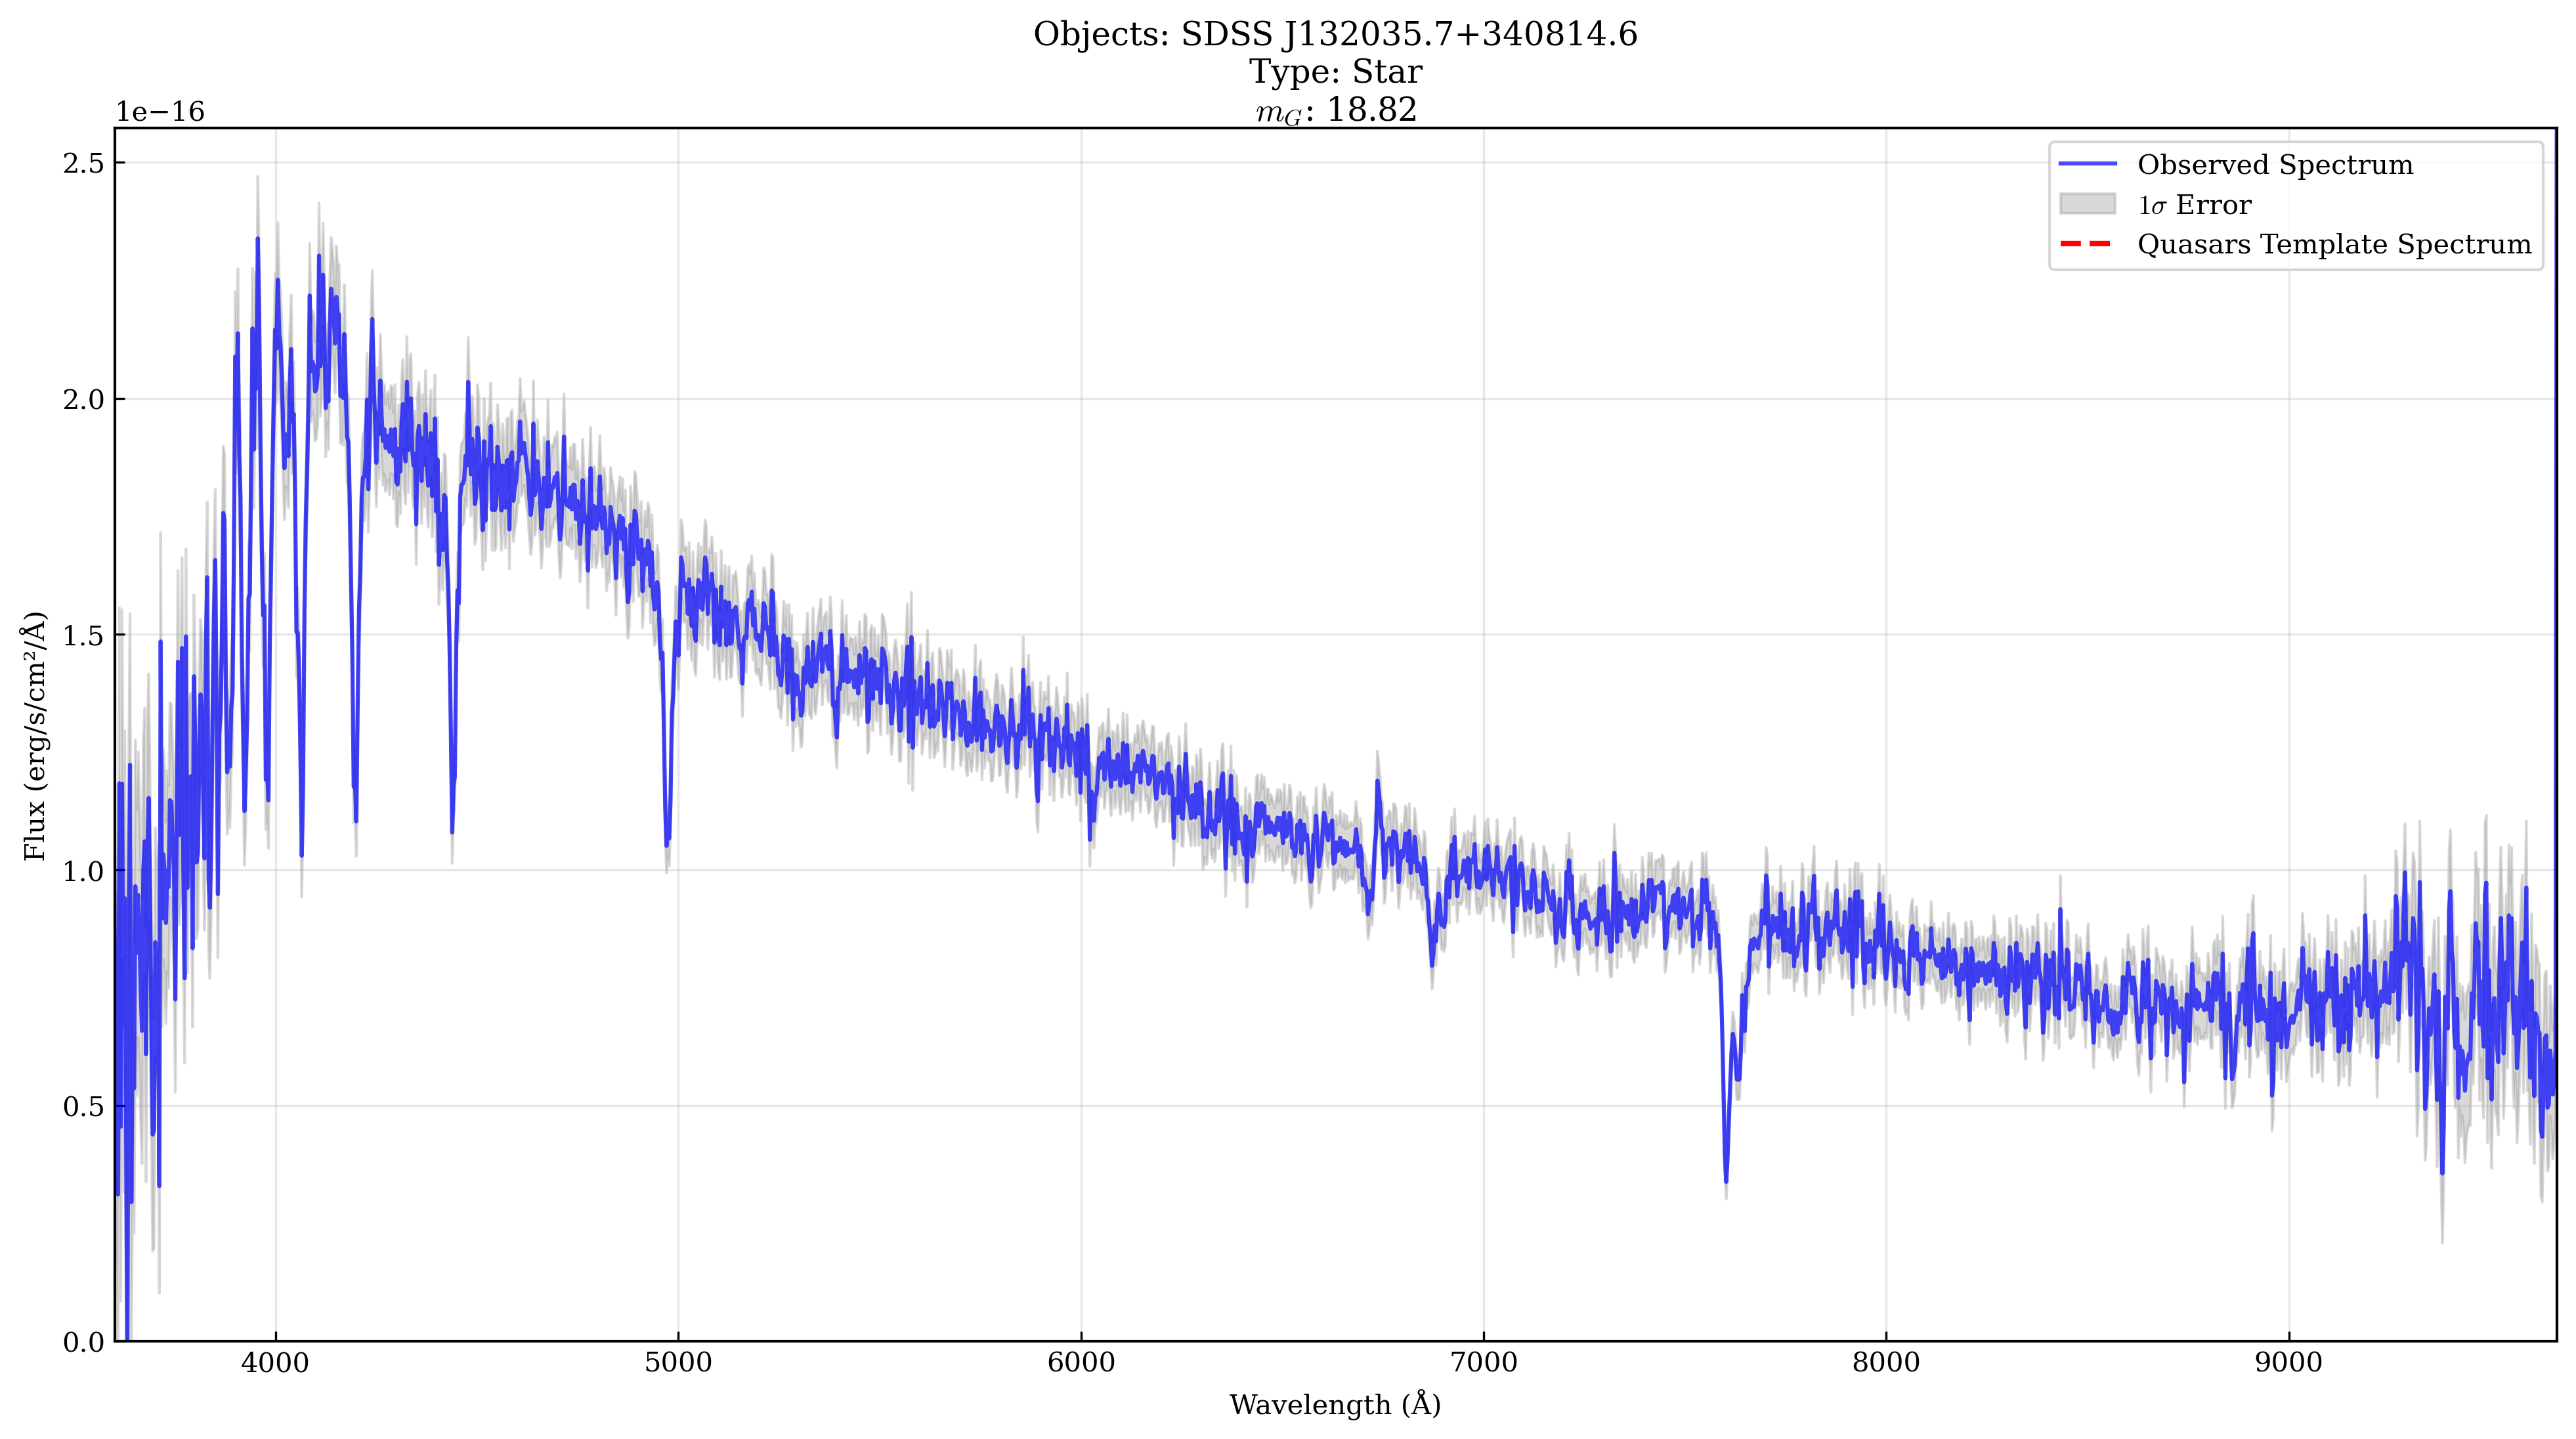
\includegraphics[width=0.9\linewidth]{figs//raw/SDSS_J132035+340814.png}
    \caption{The Spectrum of \textbf{SDSS~J132035.7$+$340814.6}}
    \label{fig:star_cluster}
\end{figure}

We also used Python package \texttt{Bagpipes} \citep{carnallInferringStarFormation2018,carnallVANDELSSurveyStarformation2019} to find the physical parameters of this cluster. We got a good result as Figure~\ref{fig:bagpipe} shows.
    
\begin{figure}[htbp]
    \begin{subfigure}[b]{0.9\textwidth}
        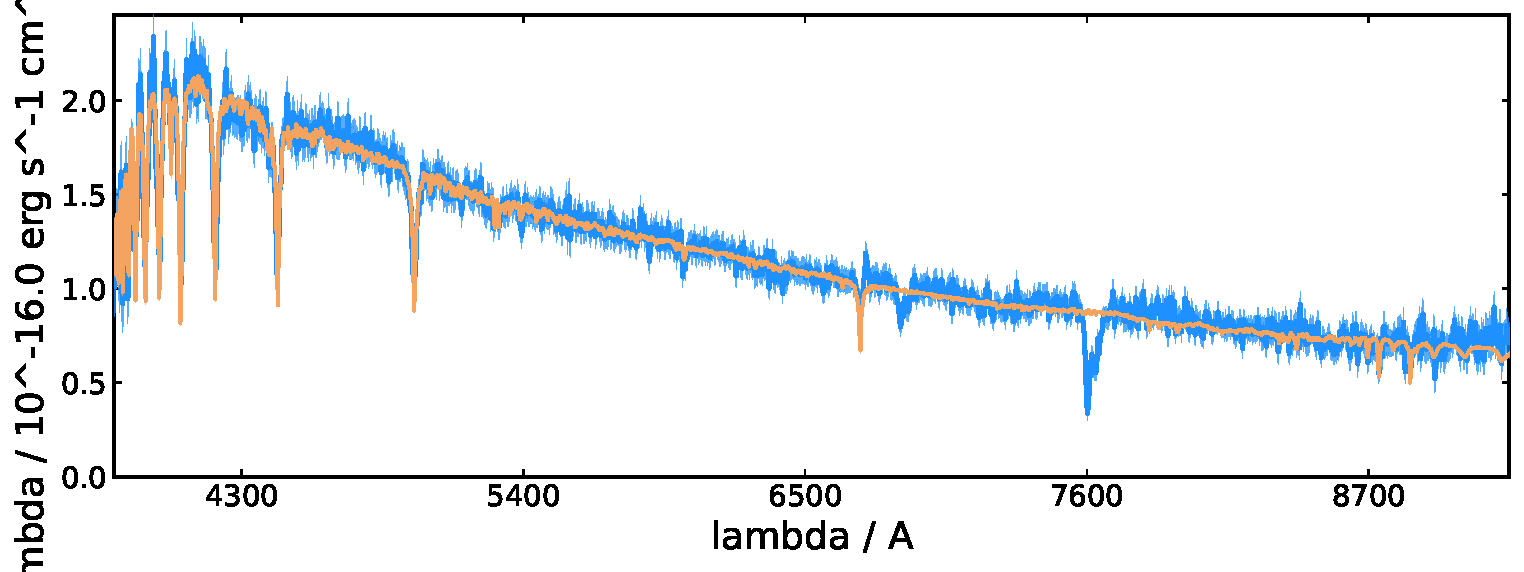
\includegraphics[width=\linewidth]{figs//res/sdssj132035+340814_combined_fit.pdf}
        \caption{Spectrum Fitting}
    \end{subfigure} \\
    \begin{subfigure}[b]{0.9\textwidth}
        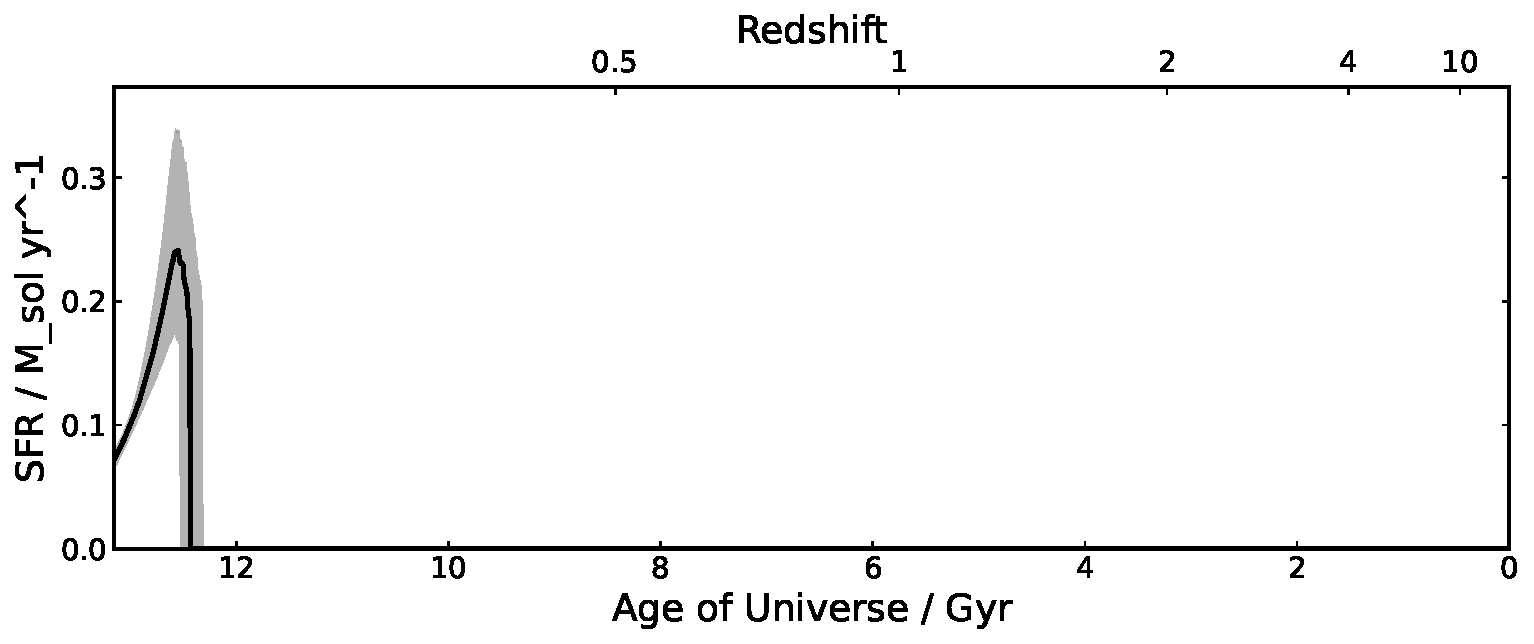
\includegraphics[width=\linewidth]{figs//res/sdssj132035+340814_combined_sfh.pdf}
        \caption{Star Formation History}
    \end{subfigure}
    \caption{Physical Parameters of cluster \textbf{SDSS~J132035.7$+$340814.6} from \texttt{Bagpipes}}
    \label{fig:bagpipe}
\end{figure}

\begin{figure}[htbp]
    \ContinuedFloat
    \centering
    \begin{subfigure}[b]{0.9\textwidth}
        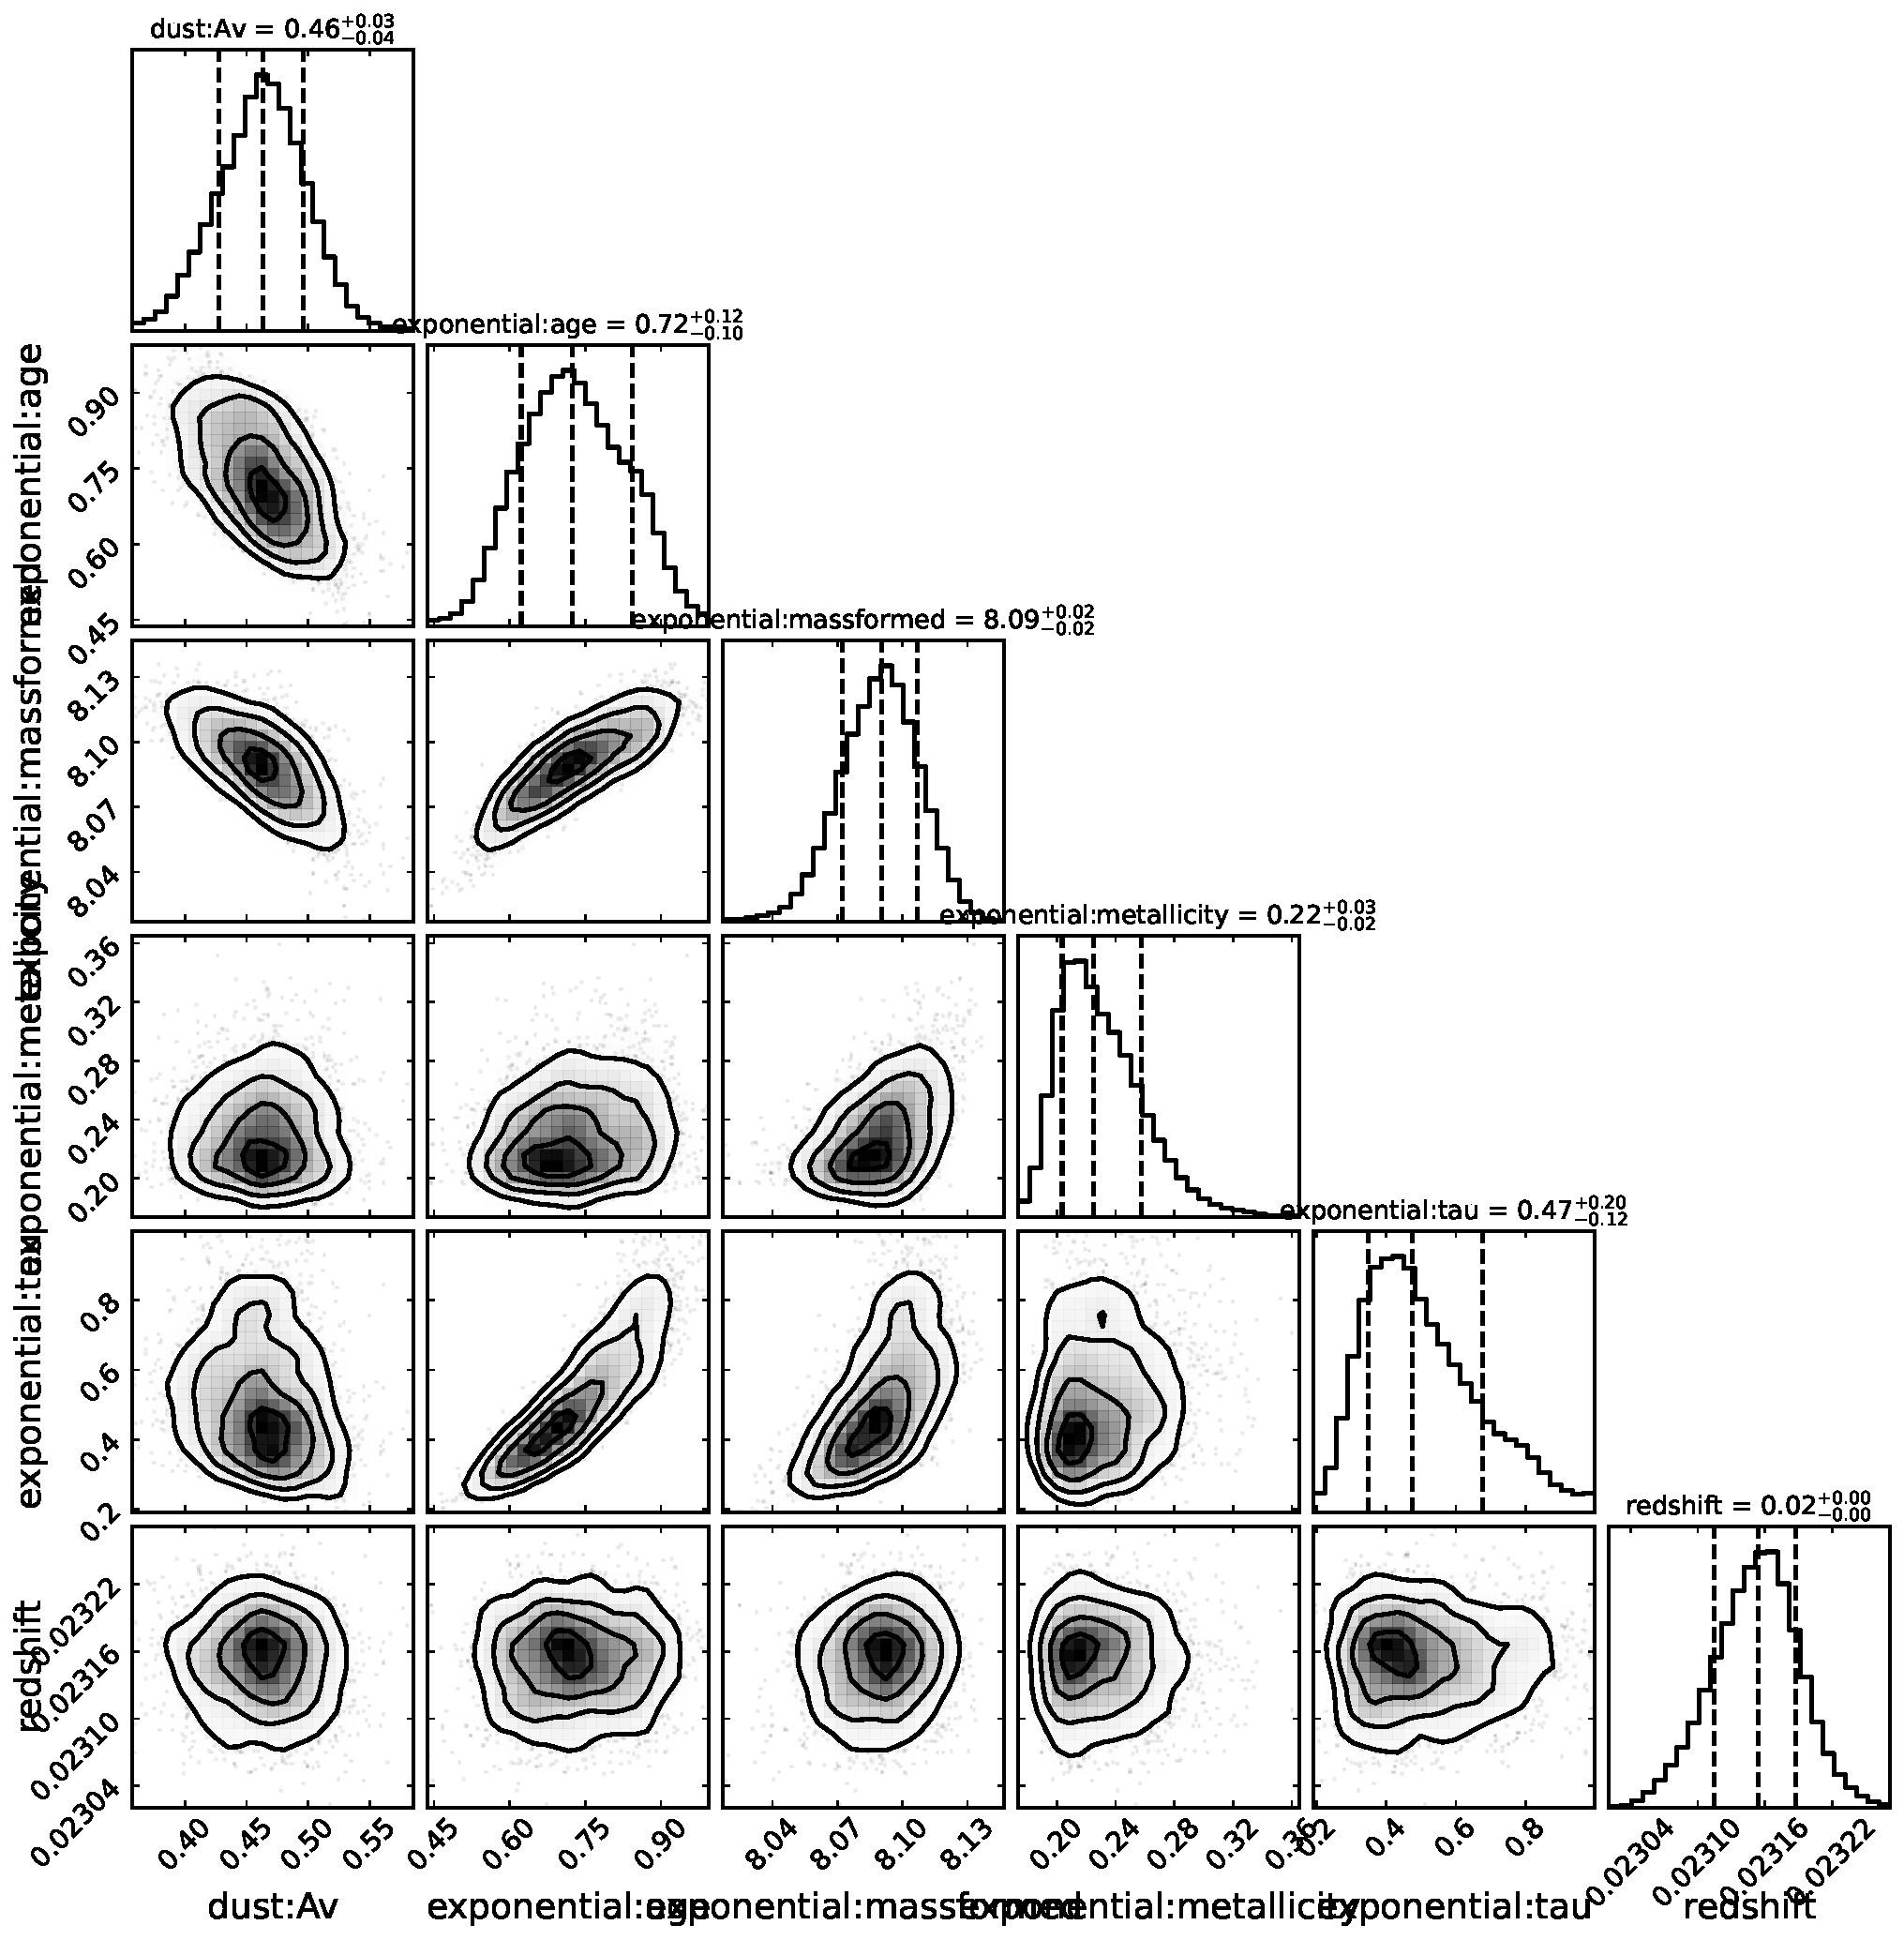
\includegraphics[width=\linewidth]{figs//res/sdssj132035+340814_combined_corner.pdf}
        \caption{Corner Figure}
    \end{subfigure}
    \caption{Physical Parameters of cluster \textbf{SDSS~J132035.7$+$340814.6} from \texttt{Bagpipes} (Countinued)}
\end{figure}


\section{The Quasars Ratio in SNAQS Selection}

Finally, we could make a summary of the quasar ratio in SNAQS Selection. A source is designated as a confirmed quasar if it is spectroscopically classified as a 'QSO' in at least one of the SDSS~DR19, LAMOST~DR11 or DESI~DR1 catalogues (\textbf{Note:} These classifications rely entirely on automated pipeline outputs and have not been visually verified. So this number must be higher than the realistic one). After merging these records from other surveys with the SNAQS observational results and 15 records from NED, then removing duplicate entries, we determine the final quasar fraction for SNAQS selection. There are \num{1393} quasars in \num{1597} targets with existed spectra in SNAQS selection. It stands for $\sim 87.23\%$ candidates are quasars, which is matched the estimation from \citet{heintz_study_2015}.

But should be noticed again, most of these classifications (from large survey catalogues) are only the automated pipeline outputs and have not been visually verified. The actual ratio is potentially lower than the above one. It requires visual inspection to confirm the final correct ratio.


